\documentclass[a4paper,10pt]{report}

\usepackage[left=2cm,right=2cm,top=2cm,bottom=3cm]{geometry}
\usepackage{titling}
\usepackage{amsmath, amssymb, amsthm, amsfonts}
\usepackage{mathchars, mathtools, mathrsfs}
\usepackage{array}
\usepackage{parskip}
\usepackage{graphicx}
\usepackage{verbatim}
\usepackage{latexsym}
\usepackage{setspace}
\usepackage{mdframed}
\usepackage[font=small]{caption}
\usepackage{color}
\usepackage{contour}
\usepackage{placeins}
\usepackage{cite}
\usepackage[mathscr]{euscript}
\usepackage[osf]{mathpazo}
\usepackage{pgf, tikz}
\usepackage{subcaption}
\usepackage[]{algorithm2e}
\usepackage{microtype}

\usetikzlibrary{shapes,backgrounds,calc,arrows}

\setlength{\parskip}{\medskipamount}  % a little space before a \par
\setlength{\parindent}{0pt}	      % don't indent first lines of paragraphs

%UHEAD.STY  If this is included after \documentstyle{report}, it adds
% an underlined heading style to the LaTeX report style.
% \pagestyle{uheadings} will put underlined headings at the top
% of each page. The right page headings are the Chapter titles and
% the left page titles are supplied by \def\lefthead{text}.

% Ted Shapin, Dec. 17, 1986

\makeatletter
\def\chapapp2{Chapter}

\def\appendix{\par
 \setcounter{chapter}{0}
 \setcounter{section}{0}
 \def\chapapp2{Appendix}
 \def\@chapapp{Appendix}
 \def\thechapter{\Alph{chapter}}}

\def\ps@uheadings{\let\@mkboth\markboth
% modifications
\def\@oddhead{\protect\underline{\protect\makebox[\textwidth][l]
		{\sl\rightmark\hfill\rm\thepage}}}
\def\@oddfoot{}
\def\@evenfoot{}
\def\@evenhead{\protect\underline{\protect\makebox[\textwidth][l]
		{\rm\thepage\hfill\sl\leftmark}}}
% end of modifications
\def\chaptermark##1{\markboth {\ifnum \c@secnumdepth >\m@ne
 \chapapp2\ \thechapter. \ \fi ##1}{}}%
\def\sectionmark##1{\markright {\ifnum \c@secnumdepth >\z@
   \thesection. \ \fi ##1}}}
\makeatother



%%From: marcel@cs.caltech.edu (Marcel van der Goot)
%%Newsgroups: comp.text.tex
%%Subject: illegal modification of boxit.sty
%%Date: 28 Feb 92 01:10:02 GMT
%%Organization: California Institute of Technology (CS dept)
%%Nntp-Posting-Host: andromeda.cs.caltech.edu
%%
%%
%%Quite some time ago I posted a file boxit.sty; maybe it made it
%%to some archives, although I don't recall submitting it. It defines
%%	\begin{boxit}
%%	...
%%	\end{boxit}
%%to draw a box around `...', where the `...' can contain other
%%environments (e.g., a verbatim environment). Unfortunately, it had
%%a problem: it did not work if you used it in paragraph mode, i.e., it
%%only worked if there was an empty line in front of \begin{boxit}.
%%Luckily, that is easily corrected.
%%
%%HOWEVER, apparently someone noticed the problem, tried to correct it,
%%and then distributed this modified version. That would be fine with me,
%%except that:
%%1. There was no note in the file about this modification, it only has my
%%   name in it.
%%2. The modification is wrong: now it only works if there is *no* empty
%%   line in front of \begin{boxit}. In my opinion this bug is worse than
%%   the original one.
%%
%%In particular, the author of this modification tried to force an empty
%%line by inserting a `\\' in the definition of \Beginboxit. If you have
%%a version of boxit.sty with a `\\', please delete it. If you have my
%%old version of boxit.sty, please also delete it. Below is an improved
%%version.
%%
%%Thanks to Joe Armstrong for drawing my attention to the bug and to the
%%illegal version.
%%
%%                                          Marcel van der Goot
%% .---------------------------------------------------------------
%% | Blauw de viooltjes,                    marcel@cs.caltech.edu
%% |    Rood zijn de rozen;
%% | Een rijm kan gezet
%% |    Met plaksel en dozen.
%% |


% boxit.sty
% version: 27 Feb 1992
%
% Defines a boxit environment, which draws lines around its contents.
% Usage:
%   \begin{boxit}
%	... (text you want to be boxed, can contain other environments)
%   \end{boxit}
%
% The width of the box is the width of the contents.
% The boxit* environment behaves the same, except that the box will be
% at least as wide as a normal paragraph.
%
% The reason for writing it this way (rather than with the \boxit#1 macro
% from the TeXbook), is that now you can box verbatim text, as in
%   \begin{boxit}
%   \begin{verbatim}
%   this better come out in boxed verbatim mode ...
%   \end{verbatim}
%   \end{boxit}
%
%						Marcel van der Goot
%						marcel@cs.caltech.edu
%

\def\Beginboxit
   {\par
    \vbox\bgroup
	   \hrule
	   \hbox\bgroup
		  \vrule \kern1.2pt %
		  \vbox\bgroup\kern1.2pt
   }

\def\Endboxit{%
			      \kern1.2pt
		       \egroup
		  \kern1.2pt\vrule
		\egroup
	   \hrule
	 \egroup
   }	

\newenvironment{boxit}{\Beginboxit}{\Endboxit}
\newenvironment{boxit*}{\Beginboxit\hbox to\hsize{}}{\Endboxit}

\thispagestyle{empty}

\setlength{\parskip}{2ex plus 0.5ex minus 0.2ex}
\setlength{\parindent}{0pt}

% to avoid error messages generated by "\@". Makes Latex treat "@" like a letter
\makeatletter

\linespread{1.5}
\def\submitdate#1{\gdef\@submitdate{#1}}

\def\maketitle{
  \begin{titlepage}{
    %\linespread{1.5}
    \Large Leiden University \\
    %\linebreak
    Leiden Institute of Advanced Computer Science 
    \rm
    \vskip 1in
    \par
    {\Large \bf \@title \par}
  }
  \vskip 0.3in
  \par
  {\Large \@author}
  \vskip 1in
  \par
  {\Large \textit{Supervised by}}
  \vskip 0.1in
  \par
  {\Large Professor A}
  \vskip 0.02in
  \par
  {\Large Professor B}
  \vskip 1.2in
  \begin{center}
  
\includegraphics[scale=2.5]{leiden}
  \end{center}
  \vskip 1in
  % \vskip 3in
  % \par
  Submitted in partial fulfilment of the requirements for the degree of 
  \linebreak
  Bachelor of Science in Computer Science, \@submitdate
  \vfil
  \end{titlepage}
}

\def\titlepage{
  \newpage
  \centering
  \linespread{1}
  \normalsize
  \vbox to \vsize\bgroup\vbox to 9in\bgroup
}
\def\endtitlepage{
  \par
  \kern 0pt
  \egroup
  \vss
  \egroup
  \cleardoublepage
}

\def\abstract{
  \begin{center}{
    \large\bf Abstract}
  \end{center}
  \small
  %\def\baselinestretch{1.5}
  \linespread{1.5}
  \normalsize
}
\def\endabstract{
  \par
}

\newenvironment{acknowledgements}{
  \cleardoublepage
  \begin{center}{
    \large \bf Acknowledgements}
  \end{center}
  \small
  \linespread{1.5}
  \normalsize
}{\cleardoublepage}
\def\endacknowledgements{
  \par
}

\newenvironment{dedication}{
  \cleardoublepage
  \begin{center}{
    \large \bf Dedication}
  \end{center}
  \small
  \linespread{1.5}
  \normalsize
}{\cleardoublepage}
\def\enddedication{
  \par
}

\def\preface{
    \pagenumbering{roman}
    \pagestyle{plain}
    \doublespacing
}

\def\body{
    \cleardoublepage    
    \pagestyle{uheadings}
    \tableofcontents
    \pagestyle{plain}
    \cleardoublepage
    % \pagestyle{uheadings}
    % \listoftables
    % \pagestyle{plain}
    % \cleardoublepage
    % \pagestyle{uheadings}
    % \listoffigures
    % \pagestyle{plain}
    % \cleardoublepage
    \pagestyle{uheadings}
    \pagenumbering{arabic}
    \doublespacing
}

% to avoid error messages generated by "\@". Makes Latex treat "@" like a letter
\makeatother


\newcommand{\bree}[1]{\makebox[4.1cm][l]{#1:}}

\frenchspacing



\usepackage{amsthm}
 
\theoremstyle{definition}
\newtheorem{definition}{Definition}[section]
 
\begin{document}

\thispagestyle{empty}


\includegraphics{logoleiden}


\vspace{-2.5cm}\hfill \begin{huge}\textbf{\begin{flushright} Bachelor Computer Science  \end{flushright}}\end{huge}

\vspace{3cm}
\begin{Large}
\hfill Topic modelling and clustering for error recognition in system logs


\vspace*{14mm}

\hfill Stephan van der Putten $(S1528459)$ 
\begin{flushright} Informatica \& Economie \end{flushright}
\end{Large}

%\vspace*{4.5cm}

\begin{large}

\vspace{2.8cm}
Supervisors:\\
Matthijs van Leeuwen \& Marcel Kolkman


\vspace*{2.8cm}

BACHELOR THESIS

\vspace*{5mm}
Leiden Institute of Advanced Computer Science (LIACS)\\
\texttt{www.liacs.leidenuniv.nl}\hfill 17/08/2018
\end{large}



%\preface
%\addcontentsline{toc}{chapter}{Abstract}
\newpage
\begin{abstract}
Our data is a collection of server logs. The servers logs have been aggregated but have no labels to indicate what type the servers logs are. This thesis focuses on the discovery and clustering of these server logs. The focus has been on logs with the term 'error'. 
The research makes use of the unsupervised machine learning technique Latent Dirichlet Allocation (LDA). We extract the server logs, transform them using the standard data preprocessing pipeline. With that we created a dataset which we can call the corpus and the logs are the documents. 
Using the best practices from Blei the founder of LDA, we create multiple models only varying in the topic count. The models are evaluated using multiple metrics. Topic modelling can distinguish itself by being one of the few machine learning techniques which depends on human readability of its models. We take a look at the topics generated by the models and conclude that a human has a hard time understanding the topics. Clustering the documents based on their highest probable topic, shows that models only have a few dominant topics where the bulk of the documents go. The clustering has a great performance based on silhouette coefficient on lower levels. At the end of the thesis we do not recommend topic modelling for latent topic discovery on server logs. Topic modelling is not human readable on server logs and applying semantic analysis metrics does not help a lot. The clustering however appears to create solid clusters when using low topic counts.
\end{abstract}


\thispagestyle{empty}

%
%\cleardoublepage

\addcontentsline{toc}{chapter}{Acknowledgements}

\begin{acknowledgements}

Here you may thank your supervisors, your family, ...


\end{acknowledgements}



\tableofcontents
\thispagestyle{empty}
%Some (very few) people like a list of tables:
\listoftables
%And some (even fewer) like a list of figures:
%\listoffigures


\clearpage
\setcounter{page}{1}

\chapter{Introduction} \label{ch:introduction}
The intention of this research started with analysing the system logs to help create a model for predicting hardware and software failure for maintenance and automatic self-healing. The huge amount of system logs available from a variety of systems brought the question how to analyse and make use of the logs to predict hardware and software failure.

Current research of big data makes this a suitable problem to solve through recent machine learning techniques. 
During the time spent on this research challenges were met and identified for realising this goal and ended with the usage of Natural Language Processing (NLP) and unsupervised learning.  The untapped amount of raw data makes it possible for many more application, but in further paragraphs it will be made clear why NLP was chosen and what more could be applied on this Big data problem.
 
 
\section{Motivation}


\section{Objectives}


\section{Research question}
How do we define similair messages?

Can we cluster these error messages to find patterns?


\textbf{Can we make a reliable model for error detection in system logs?}

\section{Eva}
 
\section{Thesis Overview}
It is recommended to end the introduction with an overview of the thesis. This chapter contains the introduction; Chapter~\ref{ch:definitions} includes the definitions; Chapter~\ref{ch:relatedwork} discusses related work; Chapter~\ref{ch:evaluation} evaluates the contributions; Chapter~\ref{ch:conclusions} concludes.

Also make a nice sentence with ``bachelor thesis'', LIACS and the names of the supervisors.



\chapter{Research Background}  \label{ch:theory}

\begin{comment}
\section{definitions}
\end{comment}

In this chapter, related work will be described. In section \ref{theory:relatedwork}, research conducted on twitter tweets and cyber security are reviewed. In section \ref{theory:featureextraction}, research that has been conducted on extracting and transforming logs to features are described. Section \ref{theory:machinelearning} introduces the previous applications of topic modelling on system logs. The last section \ref{theory:buildingblocks} introduces the tools and frameworks applied during this research.

\section{Topic modelling in general} \label{theory:relatedwork}
In this section, we briefly describe two researches that applied topic modelling. The descriptions will end with an overview explaining which parts are relevant to our current research. \par

\setlength{\parindent}{3ex} A research conducted in 2011 makes use of the numerous amounts of tweets on Twitter. Twitter is an online platform used to message about social media and news. Users make posts called \" tweets\" that are restricted to 140 characters. The authors are interested in finding news topics from twitter feeds and comparing the topics with traditional news feeds using LDA.

The data is prepared using 3 months worth of tweets and news feed data from New York Times. The tweets are filtered on stop words and tweets appearing more than 70\% of the time and less than 10 times are removed. Following the 

The authors use LDA for their topic distillation, however the data presents a problem. LDA does not perform very well on small tweets. The authors introduce a Twitter-LDA model, 


By comparing a traditional news source with
Topic modelling is a very popular and high researched field. While topic modelling  
An interesting adaptation of topic modelling can be found in twitter and cyber security. Twitter is a interesting field of research with real time tweets and a huge community. Due to the nature of twitter, analysing the huge stream of tweets can be a challenging and exhaustive task. A model with LDA has been introduced to analyse and detect topics. This model is an interesting way to provide news feeds even quicker then traditional news sites \cite{Zhao2011ComparingModels}. Cyber security has also been an area which LDA seems applicable to. Through the usage of Big data and combination of LDA, users could be identified through system and network logs. Using the event logs to identify topics, new events of users could be identified as malicious or normal \cite{Jingwei2014KnowledgeLDA}. 

To do: similar work 

\section{Feature extraction from Logs} \label{theory:featureextraction}
Logs are created in different kind of types, e.g. server logs, event logs and a lot more. The servers logs in the data set are streamed using Apache NiFi. Logs can be numerical data, but also contain non-numerical data. The messages confined in logs are textual and as such can be analysed through Natural Language Processing.
The data that logs can include can be numerical data and non-numerical data



\section{Machine learning} \label{theory:machinelearning}
In the field of computer science, machine learning is used to learn computers to classify or predict without explicitly being programmed to do so. Generally machine learning can be divided in supervised, unsupervised and reinforcement learning. The dataset that has been acquired 
The main goal of this paper a form of unsupervised machine learning.
Learning can be done supervised, unsupervised and semi-supervised. Supervised learning makes use of labeled data, which makes it easy to train and evaluate the model. Unsupervised learning makes use of unlabeled data by recognizing patterns in the data. Semi-supervised learns using both unlabelled and labelled data.
 

\subsection{Clustering Techniques}

\subsection{Hard and Soft clustering}
While hard and soft clustering are both a form of clustering, this researches contains both forms. The results discussed in chapter \ref{ch:result} contains results based both upon hard and soft clustering. Clustering data can be achieved by giving every element of the data at most 1 label, this is called hard clustering. Soft clustering allows data to be part of multiple clusters or contain multiple labels. Especially when talking about topic modelling, every document is a mixture of multiple topics this by itself is already a form of soft clustering. To avoid confusion what this research means with clustering, this section was added.

\subsection{Evaluation Techniques}

\section{Buiding blocks} \label{theory:buildingblocks}
This section has an oversight of the main tools and packages used. This section might be mentioned or referenced in later parts of this paper. The packages were required for the extraction, loading and transforming the data in an usable form.

\subsection{Packages and libraries}

\begin{enumerate}
    \item \textbf{Hadoop} $($\url{http://hadoop.apache.org/}$)$ \\
    The Apache Hadoop software library is a framework that allows for the distributed processing of large data sets across clusters of computers using simple programming models. 
    \begin{enumerate}
        \item \textbf{HDFS} $($\url{http://hadoop.apache.org/}$)$ \\
        A distributed file system that provides high-throughput access to application data. Used to store big data.
        \item \textbf{Apache Spark} $($\url{https://spark.apache.org/}$)$\\
        Apache Spark is a fast and general engine for large-scale data processing.
        \item \textbf{Apache Zeppelin} $($\url{https://zeppelin.apache.org/}$)$ \\
         Web-based notebook that enables data-driven, interactive data analytics and collaborative documents with SQL, Scala and more.
    \end{enumerate}
    
    \item \textbf{Scikit-learn} $($\url{http://scikit-learn.org/}$)$ \\
    The Scikit-learn package contains tools for effici\"ent data mining and data analysis with machine learning in Python.
    \begin{enumerate}
        \item \textbf{Pandas} $($\url{http://pandas.pydata.org/}$)$ \\
        Pandas is a library providing high-performance, easy-to-use data structures and data analysis tools for the Python programming language.
        \item \textbf{Numpy} $($\url{http://www.numpy.org/}$)$ \\
        Numpy is a scientific package with Python for powerful array objects, functions and lots of mathematical capabilities.
        \item \textbf{Matplotlib} $($\url{http://matplotlib.org/}$)$ \\
        Matplotlib is a 2D Python plotting library very similar to MATLAB.
        \item \textbf{Seaborn} $($\url{https://seaborn.pydata.org/}$)$ \\
        Seaborn is a Python visualization library based on matplotlib. It provides a high-level interface for drawing attractive statistical graphics.
        \item \textbf{pyLDAvis} $($\url{https://www.python.org/}$)$\\
        The pyLDAvis package is designed to help users interpret the topics in a topic model that has been fit to a corpus of text data. The package extracts information from a fitted LDA topic model to inform an interactive web-based visualization and can be used in combination with sklearn.
    \end{enumerate}
    
    \item \textbf{Conda} $($\url{https://www.anaconda.com/}$)$ \\
    Conda is an open source package and environment management for Python. Conda allows easy setup with out-of-the-box environments for quick testing and removal of environments.
    \begin{enumerate}
        \item \textbf{Jupyter Notebook} $($\url{https://jupyter.org/}$)$ \\
        Jupyter notebook is included in the standard data science conda package. A fast web application used to create documents in Python code to easily share code and visualise data.
        \item \textbf{Python 2.7.X} $($\url{https://www.python.org/}$)$\\
        An user-friendly and elegant programming language which has a great scientific community, making Python the go to language for data science.
    \end{enumerate}
    
\end{enumerate}

\chapter{Methodology}  \label{ch:methodology}

Why did I choose my method

\begin{table}[h]
\centering
 \begin{tabular}{l l} 
 \hline
 SYMBOL & DESCRIPTION \\ 
 \hline
 $K$ & Number of Topics \\  
 $V$ & Number of words in the vocabulary \\
 $M$ & Number of documents \\
 $N$ & Number of words in the document \\
 $N_{d=1..M}$ & Number of words in document d\\
 $\alpha$ & Collection of all $\alpha$ = $ \{ \alpha_{1},\alpha_{2}, ... , \alpha_{K}\}$ \\
 $\alpha_{k=1...K}$ & Hyperparameter for dirichlet prior distribution of topic $k$ \\
 $\beta$ &  Collection of all $\beta$ = $\{\beta{1},\beta{2}, ... , \beta_{K}\}$ \\
 $\beta_{w=1...V}$ & Hyperparameter for dirichlet prior distribution of a word $w$ in a topic \\
 $\varphi_{k=1...K}$ & Distribution of words in topic $k$ \\
 $\varphi_{k=1...K, w=1...V}$ & Weight of  word $w$ in topic $k$  \\
 $\theta{d=1...M}$ & Distribution of topics in document $d$  \\
 $\theta{d=1...M, k=1...K}$ & Weight of  topic $k$ in document $d$ \\
 $z_{d=1...M, w=1...N_d}$ & Assigned topic of word $w$ in document $d$\\
 $Z$ & Topic of all words in documents \\
 $w_{d=1...M, w=...N_d}$ & Assigned word w in document d \\ 
 $W$ & Words in all documents \\ 

 \hline
 \end{tabular}
\caption{Complete notation of LDA}
\label{tab:table1}
\end{table}

\section{Topic Modelling}\label{lda:tm}
Topic models are models used to find latent topics in mostly large unstructured collections of documents. Topic modelling assumes that documents are a mixture of topics, while topics are a distribution of words. \cite{Blei2010ProbabilisticModels}. Where humans have a hard time to find a structure, topic modelling uses statistical methods for analysing words for topic discovery. This makes it possible to compare topics with each other and to find similar documents without necessarily having any prior knowledge of your documents. The application of topic modelling is wide and is very powerful, making it a very popular for exploration of data. 

The machine learning and text mining area have focused a lot on probabilistic topic models in recent years. Models like probabilistic latent semantic analysis (PLSA) and sentiment analysis are used for applications ranging from document clustering, topic modelling and retrieval systems \cite{Lu2011InvestigatingLDA}. Optimising models is a challenging task, making usage of a high range from inference e.g. variational, stochastic variational and Markov chain Monte Carlo \cite{Hoffman2016MarkovModels}. The model that is used in this research and build upon the before mentioned models will be discussed in great length below.


\section{Latent dirichlet allocation}\label{lda:lda}
In natural language processing, \textit{Latent dirichlet allocation} (LDA) is an unsupervised machine learning technique introduced in 2003 for Topic modelling \cite{Blei2003LatentAllocation}. The notation used for LDA can be seen in Table \ref{tab:table1}. LDA is part of a larger field called probabilistic topic modelling \cite{Blei2010}.

LDA makes use of a generative probabilistic model of a collection of documents \textbf{M} (corpus) to discover latent topics. Fig \ref{fig:LDA} represents the plate notation of LDA. For a more understandable model consider Fig \ref{fig:LDA_example}. The model assumes that each document \textbf{N} in the corpus consists of a mixture of latent topics. These topics are a mixture of words \textbf{W} assigned to a topic from a fixed vocabulary \textbf{V}. \textbf{Z} notates the assignment of specific words to topics. The distribution of words $\theta$ for each topic is dependent on the sensitivity of $\alpha$. The probability distribution of topics in documents $\varphi$ are depended on the sensitivity of $\beta$. The number of topics \textbf{K} are predefined by the user. 

\begin{figure}
    \centering
    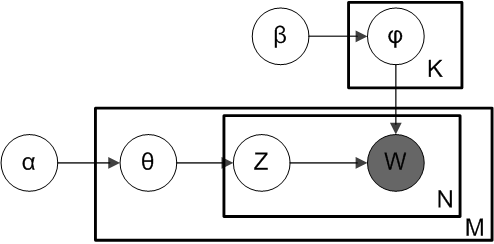
\includegraphics[width=10cm, height=5cm]{methodology/Smoothed_LDA.png}
    \caption{The smoothed LDA plate notation}
    \label{fig:LDA}
\end{figure}

The LDA model is defined in 3 steps and shown in Fig \ref{fig:LDA_example}:
\begin{enumerate}
    \item For each document, pick a topic from its assigned distribution over topics.
    \item Sample a word from the distribution over the words associated with the chosen topic. 
    \item  The process is repeated for all the words in the document.
\end{enumerate}

For a better understanding, look at the before mentioned Fig \ref{fig:LDA_example}. The topics are shown on the left side with their probability of words. On the right side, the document has a topic proportion. Every word gets assigned to a topic so that the topic proportion matches.  
In the original LDA model, assignments of words get updated every iteration through the corpus M. Restarting the process again until the LDA model converges and the topic and assignment are stale. The eventual quality of the model depends on the assumed hyperparameters $\alpha$ and $\beta$ and parameters $\theta$ and $\varphi$. For a better understanding of the parameters take a look at section \ref{lda:alphabeta} and section \ref{lda:thetavarphi}.

\begin{figure}
    \centering
    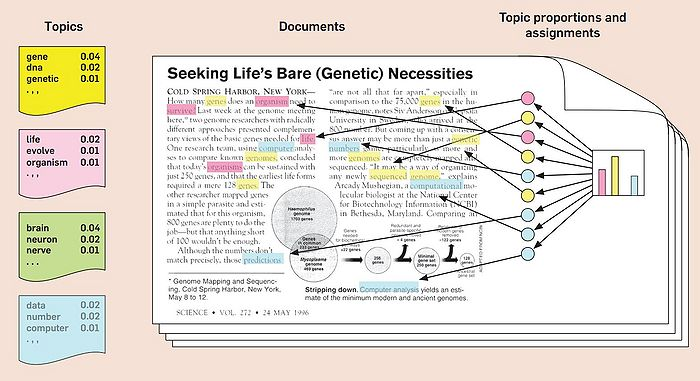
\includegraphics[scale=0.6]{methodology/700px-Illustrating_LDA.jpg}
    \caption{LDA applied to a document}
    \label{fig:LDA_example}
\end{figure}

\subsection{$\alpha$ and $\beta$ hyperparameters}  \label{lda:alphabeta}
The dirichlet is defined as the distribution over a distribution. Dirichlet is used to infer a posterior distribution after observations using a prior distribution \cite{Sethuraman2001APRIORS}. Hyperparameters are defined as parameters that assume a prior distribution before any evidence or information is taken into account. This distinguishes $\alpha$ and $\beta$ from the remaining parameters. $\alpha$ and $\beta$ are both dirichlet distributions. The hyperparameter value $\alpha$ is the parameter of the dirichlet prior on the per-document topic distributions. The result of a high value of $\alpha$ is a document with a mixture of most topics, while the low value leads to documents with more distinct topics. The $\alpha$ results in a corpus with distinct documents or more general documents topic assignments. The value $\beta$ is the parameter of the dirichlet prior of a word in a topic. A high value for $\beta$ means that the topics consists of distinct words, the low value of $\beta$ assumes topics are more generative. The $\beta$ will influence the general distribution of words in topics in the output of topics.

\subsection{$\theta$, $\varphi$ parameters}\label{lda:thetavarphi}
The parameters $\theta, \varphi$ are depend on the prior distributions $\alpha$ and $\beta$. $\theta$ is the document-topic distribution. $\theta$ is the weight of a topic in a document and because $\alpha$ is a prior distribution, $\theta$ assumes a distribution based on the previous assigned distribution. 
In the same way $\varphi$ is the weight of words in a topic. $\varphi$ in this case is dependent on the $\beta$.



\subsection{Online Latent dirichlet allocation} \label{lda:onlinelda}
The online variant of LDA was introduced  by Hoffman et al. in 2010.\cite{Hoffman2010OnlineAllocation} This new variation dealt with the problem earlier LDA models struggled with. The problem that LDA had was the computing of huge collections of documents. The online LDA can be used for massive and streaming documents without losing performance compared to the original LDA model, because it analyses the documents in batches instead of single observations with stochastic (random) optimisation.\cite{Beaver2012StochasticInference} 

\subsection{Dimensionality reduction}
LDA is widely applied for text clustering, because LDA actually reduces the dimension. Reducing the dimension with LDA then use Jensen-Shannon distance  to measure text similarity, which we discuss in chapter \ref{research:jsdivergence}. The input is usually a bag of words matrix that can be transformed to a document topic matrix. After this models like K-means can be used to cluster similar documents with each other. 

\section{Text preprocessing}
In this section we\'ll talk about the input dataset, the reason why we selected it and how it got processed for our model. Preprocessing involves tokenization and stop word removal discussed in section \ref{tokenization} - \ref{bagow}. Preprocessing is important and if done wrong can impact the final results. It\' s common knowledge that giving a model bad input brings bad output.

\subsection{Dataset}
The dataset was provided by Capgemini containing syslogs. The syslogs contains event logs from different servers provided to their customers and internal staff. The event logs used on their servers were extracted from different operating systems, ranging from the year 2015 to current day. Due to the size and complexity of the dataset, this research contains 1 day of data selected by the word error. The dataset will be refered as the corpus and the system logs as documents throughout this research. The corpus contains around 400000 records and has messages consisting of twitter like sizes. 
The documents has a few attributes, hostname, severity, port, priority, valid, protocol, body. The attribute contain little information and will not be used, only the body has been extracted which contains the event log.

\subsection{Tokenization}\label{tokenization}
In the preprocessing phase, the document needs to be transformed from a raw text to a usable vector. The nature of the documents make it possible for the same kind of messages to be represented in different ways. The goal is to extract only the usable textual data.

The content of the document consisted of the message and specific user and server information. An algorithm had to be written to remove the unnecessary information from the dataset. This filtered the message from the specific server data and removed the specific users information from the message.  To our research only the message remains relevant.

\subsection{Stop word}\label{stop_words}
LDA assumes that each word is equally important, which we can simply deduce to not be true from a logical and linguistic point of few. Words such as \' the\' and \' a\\an\' are not important, likely short words and other general English words can be removed to only keep the most distinguishable words left. The provided tools in sklearn provide a standard tokenization option with stop words from the English vocabulary.

\subsection{Bag of words} \label{bagow}
The text preprocessing in this research makes usage of the bag-of-words representation as is common for topic modelling. Bag of word counts the words that appeared in the document and represent the words in a document as as a term frequency matrix. The bag of words representation of a document doesn\' t take in the order or semantic structure in a document, but LDA discovers these semantic structures itself. 

\section{Syslog} 
Syslogs are textual messages \cite{Stearley2004TowardsSyslogs} which contain the messages provided by the systems.


\section{Challenges}

\subsection{Natural Language Processing}


\subsection{Semantics}


\subsection{Sentiment analysis}


\subsection{Extract, Transform, Load}



%\chapter{Contributions}  \label{ch:contributions}

The contribution this research brings is in the field of topic modelling and the analyses of system logs. A lot of data is collected in the past few years, this data also consists mostly of system logs. Research using datasets containing system logs are few and contain 

\chapter{Results}
\label{ch:result}

In this chapter we will discuss the results retrieved after applying our LDA implementation.

\section{Model results}

\begin{figure}[h]
    \centering
    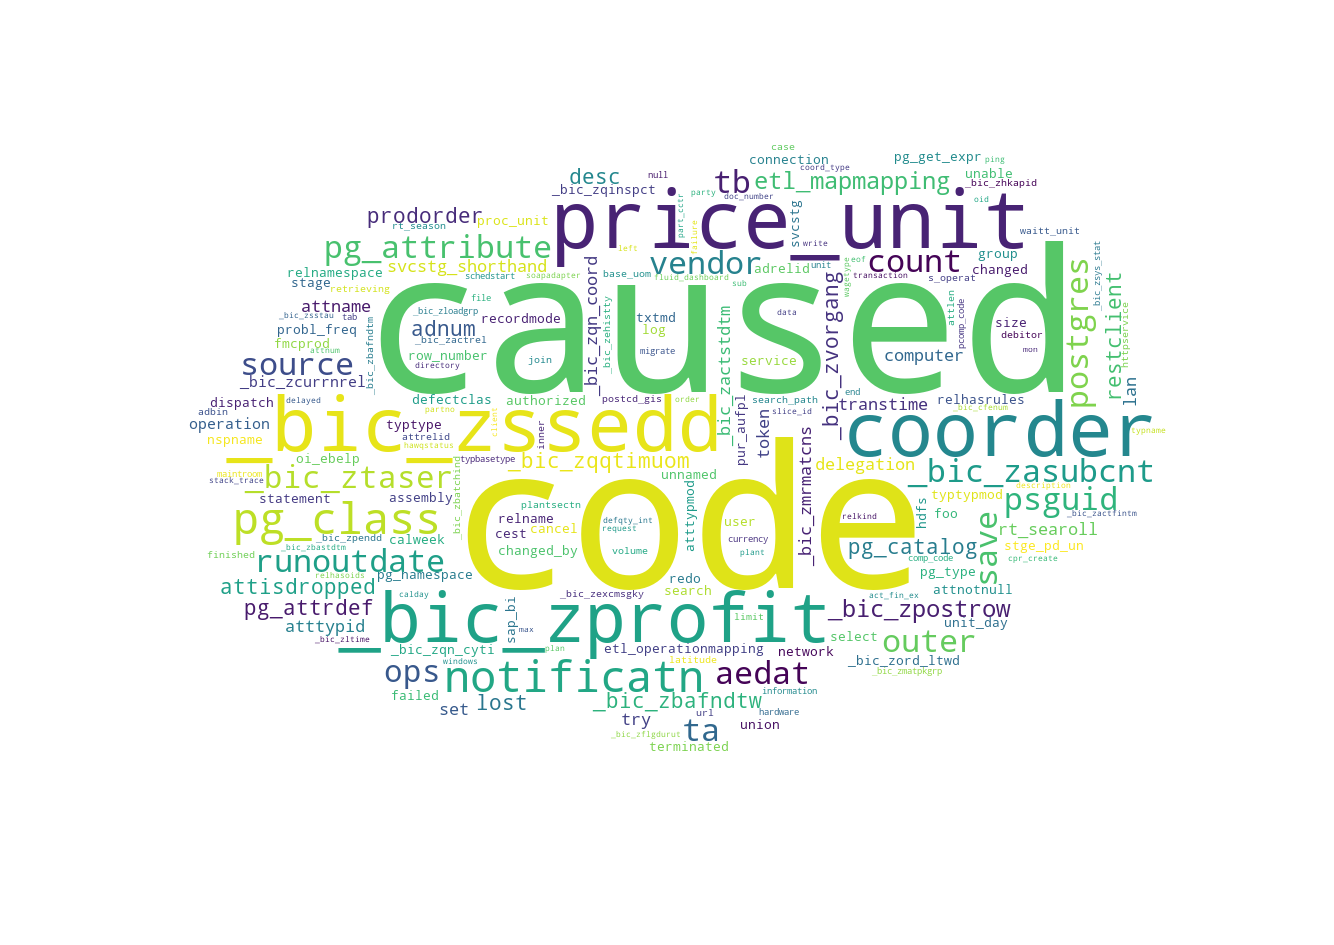
\includegraphics[width=15cm, height=8cm]{figures/wc.png}
    %\caption{The smoothed LDA plate notation}
    \label{fig:worldcloud}
\end{figure}

\begin{comment}

The model used is ofcourse LDA.

\end{comment}

\section{Evaluation Measures}
To evaluate our implementation we use different metrics. Evaluating an unsupervised learning model depends on the application and the goal the model is made with. In our case the metrics are here to evaluate the models capability to generalise, using perplexity. The clusters are evaluated based on their inner similarity between documents and \" distance \" compared to other cluster centroids, using Silhouette co\"efficient. The distance metric used for silhouette co\"efficient is based on the KL-divergence metric. Human perception is also an important factor to evaluate the models, which isn't used in this research but we will discussion shortly.

\subsection{Perplexity}\label{research:perplexity}
In the original paper Blei introduces a general model evaluation metric \cite{Blei2003} to compare topic models. Perplexity can be used to compare the generalisation of a model on new unlabelled data.

\[
   \mathlarger{perplexity(\textbf{D}_{test}) = \exp{\Bigg \{ -\frac{\sum{}_{d=1}^{M}logp(\textbf{w}_d)}{\sum{}_{d=1}^{M}N_d} \Bigg \}}}
\]

Perplexity shows the perplexity on the test set of held out documents $\textbf{D}$. The nominator shows the sum in  corpus $M$ with document $d$, where the likelihood of each word in d is computed. The denominator consists of the count of words $N$ in document $d$.
The lower the perplexity score the better a model generalises. 


\subsection{Silhouette coefficient} \label{research:silhouette}
The silhouette is used to measure between the cohesion and the separation of intra-clusters. In our model this measures the mean intra-cluster distance for each document and compares distance to the nearest-cluster distance.

\[
   \mathlarger{s(i) = \frac{b(i) - a(i)}{\max{\{ a(i), b(i)}\} } }
\]

Where $s_i$ is the silhouette of sample $i$ in the cluster. $a_i$ is the average distance for $i$ from all the objects in the cluster and $b_i$ the distance of $i$ from a cluster $b$ not containing $i$. 

\[
\mathlarger{-1 \leq s \le 1}
\]

The value of $s$ will be contained between $-1$ and $1$. If $s(i) = 1$ then we can say that the distance $i$  is a lot less in its own cluster then the nearest other cluster. If we take $s(i) = -1$ then the similarity of $i$ is higher in the other nearest cluster then its current cluster \cite{Rousseeuw1987Silhouettes:Analysis}.


\subsection{Jensen-Shannon divergence and KL-divergence} \label{research:jsdivergence}
The Kullback Leiber divergence was introduced to measure the density between to distributions \cite{Hershey2007ApproximatingModels}. Based upon this important and popular measure the Jensen-Shannon divergence (JS) was introduced \cite{Fuglede2004Jensen-ShannonEmbedding}. Which is better used to measure similarity between two text documents based on their probability distributions.

\[
\mathlarger{JDS(P||Q) = \frac{1}{2}D(P||M) + \frac{1}{2}D(Q||M)}
\]

Where $P$ and $Q$ denote a probability distribution and $M$ the set of probability distributions. The useful if especially to find the distinctiveness and cohesion between topics

\subsection{Human perception}
Although LDA can be used to find latent patterns, explore, tag recommend in a document corpus the final result of topics do not necessarily match up with the human expectation of a topic. Especially in a unsupervised learning model with only mathematical measures\cite{Towne2016MeasuringPerception}. The reason of this paragraph is to make readers aware that the suitability of a model in a unsupervised learning and NLP environment still need support of a human factor. Research from Chang  et al. \cite{Chang2009ReadingModels} and Blei et al. \cite{Chaney2012VisualizingModels.} provide more indepth research in this topic.

\subsection{parameter tuning}
During the experimental phase. The research coneducted sucked, but Althought it sucked we got somewhere. 

\section{Graphs of results}

\begin{comment}
Visualizing the messages is really fun!
\end{comment}

\section{Contribution}

\begin{comment}
I dont think I contributed a lot to the research in this area, but I learned a lot right??
\end{comment}


\chapter{Conclusions} \label{ch:conclusions}
This chapter contains the conclusion in which we will shortly explain the research and derive a conclusion from our experiments. We will answer the research questions and end the chapter with a section discussion and future work.

\section{Conclusion}\label{conclusion:clonclusion}
This research aimed to apply topic modelling for clustering and discovering an optimal model with the help of server data of Capgemini. Capgemini provided data of their server data warehouse for this research. We extracted a subset of data contained in the server logs filtered on the term 'error'. Based on earlier research we use the unsupervised machine learning model Latent Dirichlet allocation (LDA) to discover latent topics in this data set. As such we recognise our dataset as a corpus and the server logs as the documents in this corpus. To achieve this transformation of data to corpus we used some steps.
We preprocessed the data using the standard steps: normalisation, stop word removal, tokenization and creating a bag of words matrix (bow). The bow was divided in a train, test and held out set. Furthermore, we trained multiple models with different amounts of topics {2-38} with our train and test set. Lastly we evaluate the results of each model using multiple metrics. We evaluate distinctiveness, coherence of each topic using pyLDAvis and the coherence metric Cv. We further use human perception to evaluate the topics with their top terms. The documents are clustered based on their highest probable topic and as such we compare the document distribution based on hard clustering. Finally we use the silhouette coefficient to compare the multiple topics. 

We will answer each research question and end with answering our main research question based on the results and the best of our knowledge.

\subsubsection{How does the topic count influence the topic models?}
During this thesis we applied many steps to our data. We chose multiple topic counts using the standard preset the gensim package offered us. For this research we created 25 models with the help of 380000 documents to train and test and the remaining documents to validate the models. Each evaluation measure shows a different side of our models. If we go back to our goal of discovering latent patterns and clustering documents we can explain our results. Our first observation of the pyLDAvis with a topic overview make it clear that the topics are hard to deduce. With pyLDAvis helping us to look fo extra, we see that increasing topics create more overlap of terms. The coherence that we see in Fig \ref{fig:coherence} shows no clear winner, however once again increasing the topic count too much makes the quality even more unpredictable. The contrasting results make it hard to judge these models on quality. Furthermore, when comparing our clustered documents in Fig \ref{fig:doc_distr_1-11corpus} and the remaining distribution we can see that the topics generally stay around 2-3 large clusters, interestingly increasing the topic count flattens the distribution of documents, with at least 1 topic mostly having the largest cluster. The silhouette clearly indicates that higher topic counts have simply to much overlap which makes it not calculable, however lower topic counts show high silhouette scores. The results leave no conclusive decision, but we can say that the higher the topic count the less the quality of the overall clustering. The contrasting results of coherence and pyLDAvis makes it not clear whether interpretability increases with higher topic count for the topics and leaves us inconclusive.

\subsubsection{Why are the chosen topic models suitable?}
In the earlier part of this thesis we analysed multiple researches each with their own implementation of LDA. Our dataset is based on the optimal parameters Blei researched. While we do not have a streaming corpus, the online implementation of LDA that we applied in our thesis allows the models to be updated with new documents. This allows our current models to learn new terms and be able to cluster unseen documents better. This makes our models suitable for future recognition of error logs.
    
\subsubsection{What are our findings when applying topic modelling and optimising the model on our data?}
Evaluation is really hard on topic modelling. Especially when the data is so domain specific. Server data is not the same as natural language and using topic models will not result in clear topics from each model. Our human minds can see some connection between current logs, but we clearly do not possess the skills to interpret the topics objectively. It is simply to hard for a human to deduce the topics with our current dataset and models, which is why a unsupervised machine learning technique as LDA is really optimal to recognise the correlations using semantic analysis.

\noindent Leaving us with the research question.

\subsubsection{\textbf{\textit{Can we use topic modelling to classify and cluster error messages?}}}

When all is said and done. Topic modelling can be used to analyse great deals of documents, discovering latent topics and clustering new unseen data in a similar way. However, the application of topic modelling on a dataset which is not even human interpretable makes the results afterwards hard to evaluate. If our application were to be to recognise error messages, this model would be up to the task. The model is even able to be updated. The clusters would be based on the scores of silhouette very good coherent and distinct from other clusters. Which once again begs the question, can we recognise the topic we put our new document under? It is not very useful to cluster documents together without understanding the topic this document falls under. The interpretability of topics leaves much to be desired. With the measures we used to evaluate our models, we would not recommend using LDA for classifying and clustering error messages. Topic modelling is better of being used on normal human generated corpora.

\section{Discussion}

\subsection {Methodology considerations}
This research took only a small possible path in the finite amount of paths. This section will further explain this path, which led this research to its logical conclusion and a honourable mention to not forget the time spent.

\subsection{The reason leading up to LDA}\label{conclusion:discussion}
Although the discussed research has been mainly focused around topic modelling (LDA) on finding similar error logs, the original research question started with a related but different subject. During this section I would like to discuss the original focus of predictive maintenance, as a lot of time has also been put in researching this difficult and challenging task. 

\subsubsection{Predictive maintenance}
With the combined application of machine learning and big data, companies try to anticipate when machine hardware failure are due to occur. Predicting instead of reacting to problems saves time and money and allows for a better customer experience which can be found in the before mentioned research of Intel \cite{Sipos2014Log-basedMaintenance}\cite{AjayChandramoulyRavindraNarkhedeVijayMungaraGuillermoRueda2013ReducingAnalytics}. It is not hard to imagine why companies like Intel  or Google have already been researching the possibility of big data for this problem. Which brings us to the data acquired for this thesis, originally intended by Capgemini for predictive maintenance. 

\subsubsection{Vrops and syslogs}
The data had not only been system logs but also consisted of vrops logs. In a few words, vrops are unstructured logs created by the virtualisation tools of VMware. The vrops data contained health and performance statistics of their multiple servers. Extracting the values from the vrops databases with the Hadoop framework had great promise to lead to the desired research data necessary for predictive maintenance. Furthermore the syslogs contained an indication of the type of log. Early examination of these logs, brought  messages from all kinds of type of servers. The following step was to understand and extract the data to use in our research.

\subsubsection{Unlabelled and unstructured}
Unluckily we soon enough found the syslogs to be lacking their log type. This seemed to be a mistake made by their developers when implementing their streaming pipeline of server logs, which made the data set of the last three years unclear of their type. This in turn made it impossible to use the vrops values, which could be understood combined with the syslogs, to correctly to know when system problems would occur, without having a consulting a domain expert all the time. The only logical step was to find a more mathematical suitable way to label the unlabelled and unstructured data, bringing this research again to the literature study phase for a new solution.

\subsubsection{Topic modelling}
Going back and forth between different algorithms available, my supervisor finally hinted at Latent Dirichlet allocation (LDA). Lots of research has been done with LDA. Having already been wasting enough time on searching, this research had to settle for a technique. LDA seemed like an applicable algorithm to this problem based on earlier research. Text mining on logs has been done before, although barely on unlabelled logs. Training LDA on unlabelled data was common, expect that a lot of data contained either longer documents or a less domain specific dataset. 

\subsection{Recommendation}
In further research I would not recommend LDA for domain specific log research and labelling, unless one has enough time and patience and expertise. If one is to attempt LDA for further research on logs, be sure to know which results are wished for. Evaluating LDA without a proper desired result might leave the evaluation process as a tedious phase. 

\section{Future work}
This research leaves a lot of open areas to optimise or further research server logs in general with topic modelling. Experimenting on similar data can be achieved and as such a few points which come to mind when recommending future works are:

\begin{enumerate}
    \item The way documents and corpora are declared. The corpus in our research was 1 day of data, filtered on the term 'error'. The documents could be an collection of specific server instead of 1 log being 1 document, this will increase the document size tremendously and should help LDA perform better.
    \item The pipeline of data extraction. We filtered a lot of server specific features to extract our dataset, which can be a loss of information for LDA. 
    \item Data preprocessing. This is clearly always important when processing the data and can be experimented on in various ways.
    \item Exhaustive search. Most parameters were based on best practices from earlier performed, especially by Blei from the original LDA paper. Hyperparameters and topic count can be changed and better set based on the distribution of your documents. This can be quite exhaustive and time consuming, but could be interesting. Otherwise making use of a super computer speeds up the calculations.
    \item The quality of data. LDA is created to handle large amounts of documents, which we did have but not with the desired document length and variety. Using more varied logs, like informational logs etc could be show better latent topic inference. 
\end{enumerate}


\chapter{Appendix A} \label{ch:appendices}

\section{Capgemini server dataset}\label{appendices:serverdata}

This section serves as a complete overview of the data. The server data that is provide by Capgemini has been developed by their own developers and as such contains a custom schema. Event logs contain multiple columns shown in table \ref{tab:tableservercol} in an order fashion. Due to privacy reason, we will not show the data that is contained within the rows. Only two columns are worth discussing: syslog.body, syslog.severity. The former contained a lot of server specific data. This event log has been formatted to have a lot in common with the syslog message standard. The latter contains the type of message the event log, e.g. 0 indicating an emergency message. Due to a formatting error discovered during the research, the original syslog.severity has been lost and is always labelled 6 meaning informational. 

\begin{table}[h]
\centering
 \begin{tabular}{|l|l|l|l|l|l|} 
 \hline
 filename & hostname & mime.type & path & syslog.body & syslog.facility \\ [0.5ex] 
 \hline\hline
 syslog.hostname & syslog.port & syslog.priority & syslog.protocol & syslog.sender & syslog.severity  \\ [0.5ex]
 \hline\hline
 syslog.timestamp & syslog.valid & syslog.version & timestamp & uuid & \\
 \hline
 \end{tabular}
\caption{All the columns in the complete dataset}
\label{tab:tableservercol}
\end{table}

After manually inspecting the data we extracted only 4 columns named: hostname, uuid, syslog.body, timestamp. A custom solution had to be written to transform the servers logs into a use able matrix. These steps are explained in section \ref{methodology:dataset}. 

\FloatBarrier

\section{Pyldavis}\label{appendices:pyldavis}
The remaining Ldavis visualisation.

 \begin{figure}[!h]
    \centering
    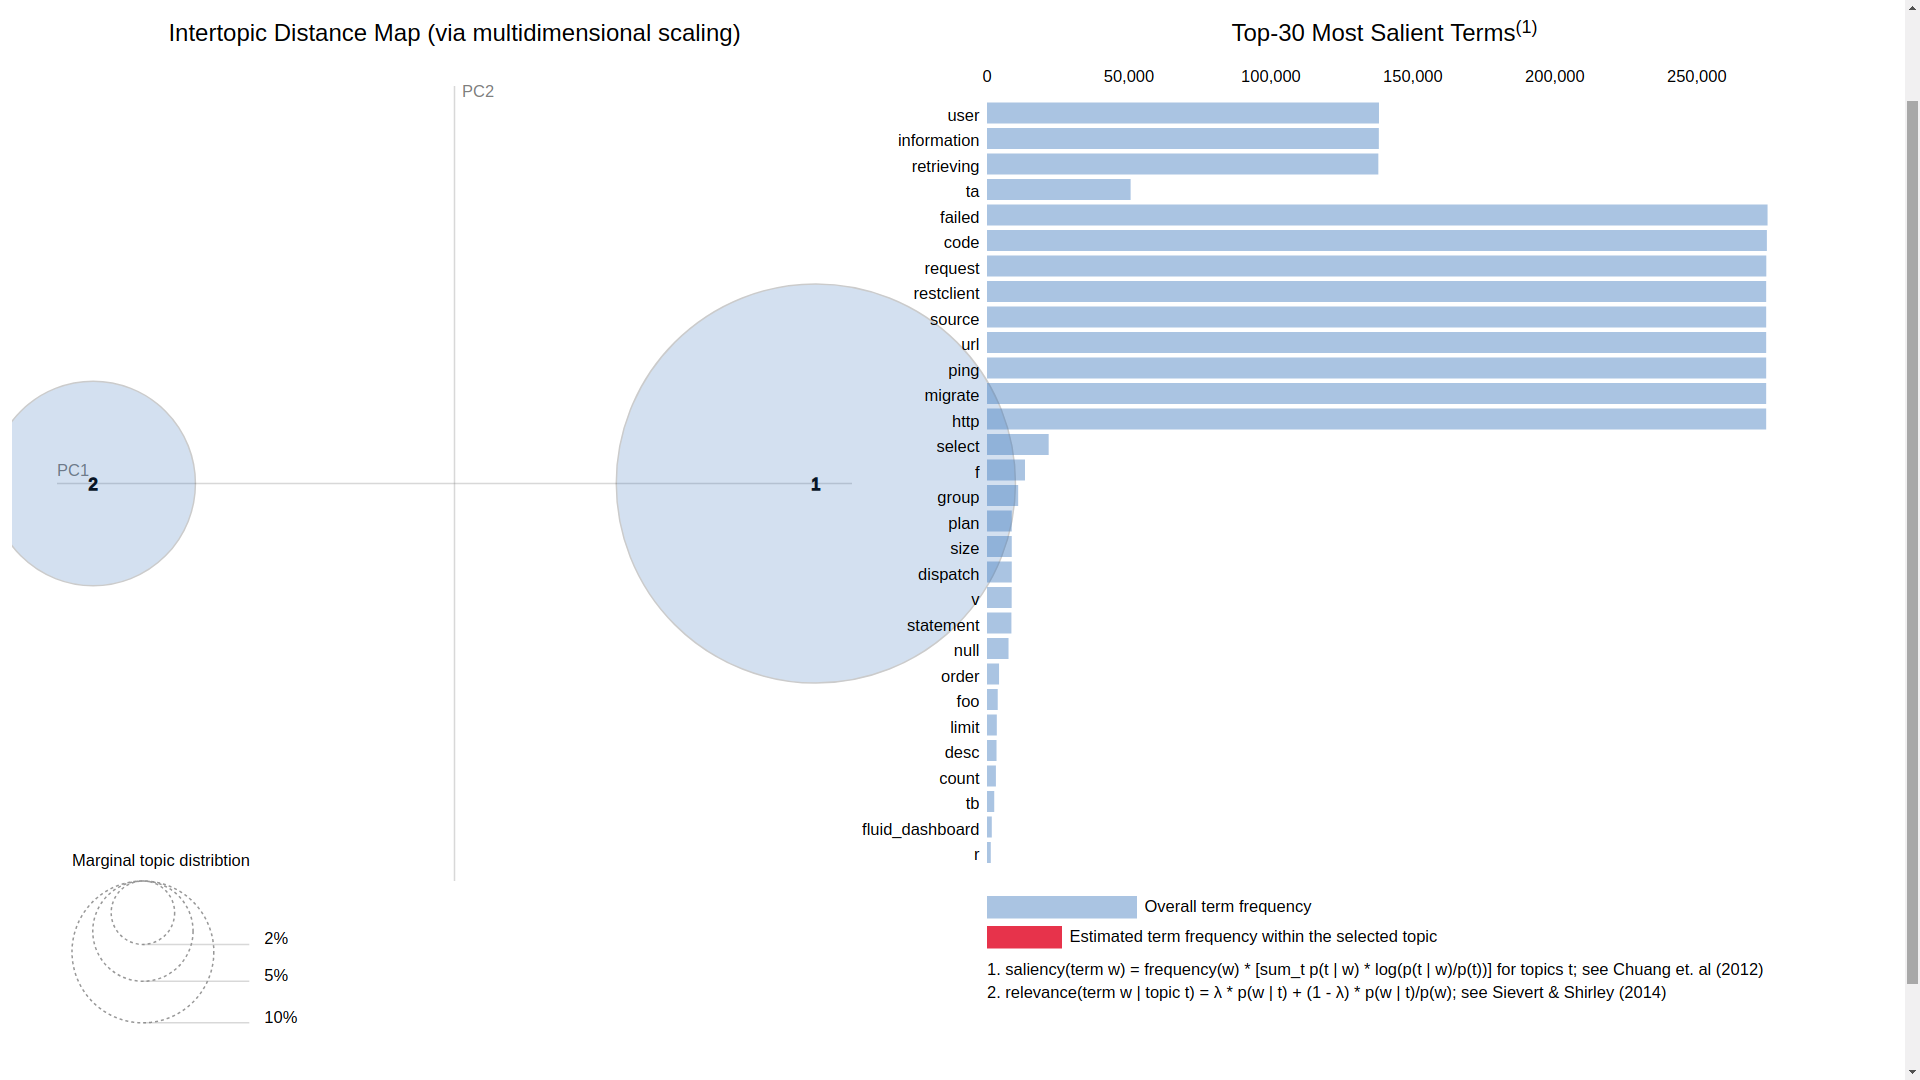
\includegraphics[width=15cm, height=8cm,trim=0 0 100px 0, clip=true]{figures/pyldavis/pyldavis_2.png}
    \caption{PyLdavis topic visualisation with 2 topics}
    \label{fig:pyldavis_2}
\end{figure}


 \begin{figure}[!h]
    \centering
    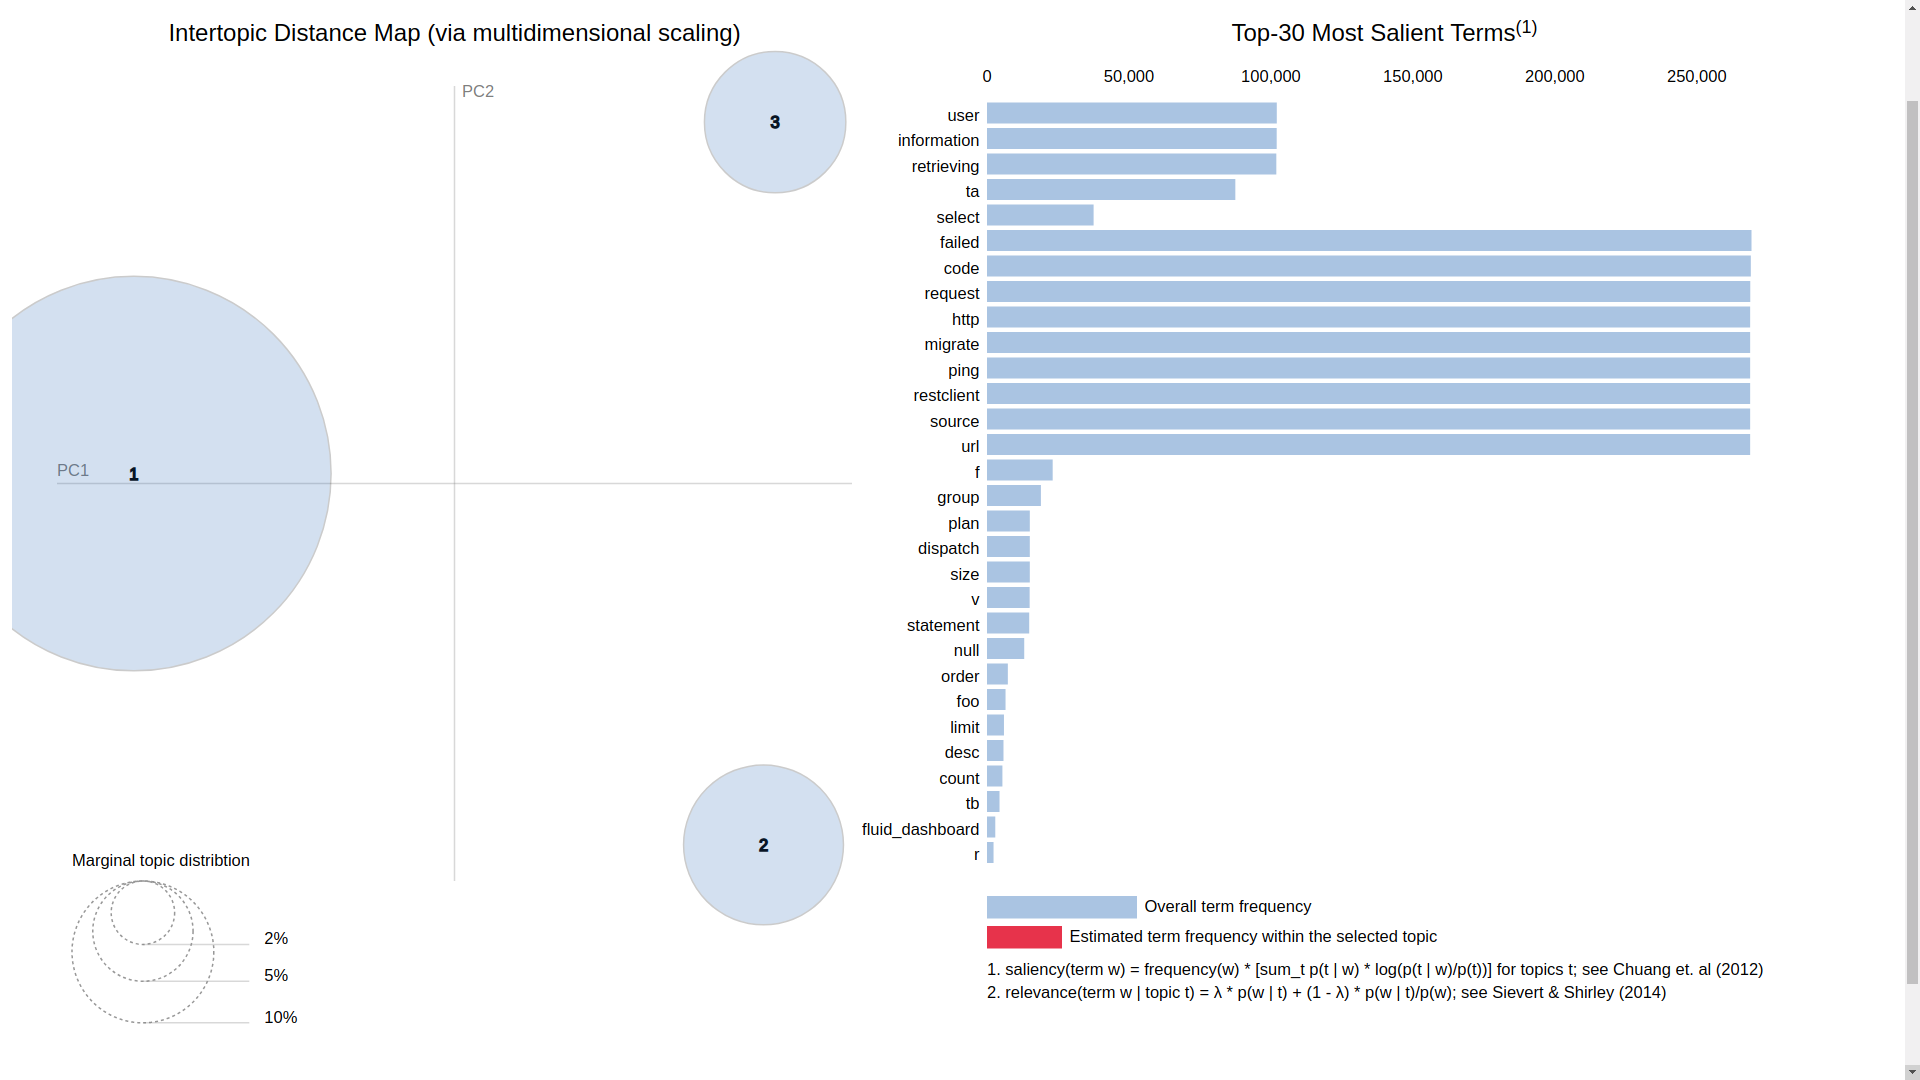
\includegraphics[width=15cm, height=8cm,trim=0 0 100px 0, clip=true]{figures/pyldavis/pyldavis_3.png}
    \caption{PyLdavis topic visualisation with 3 topics}
    \label{fig:pyldavis_3}
\end{figure}

 \begin{figure}[!h]
    \centering
    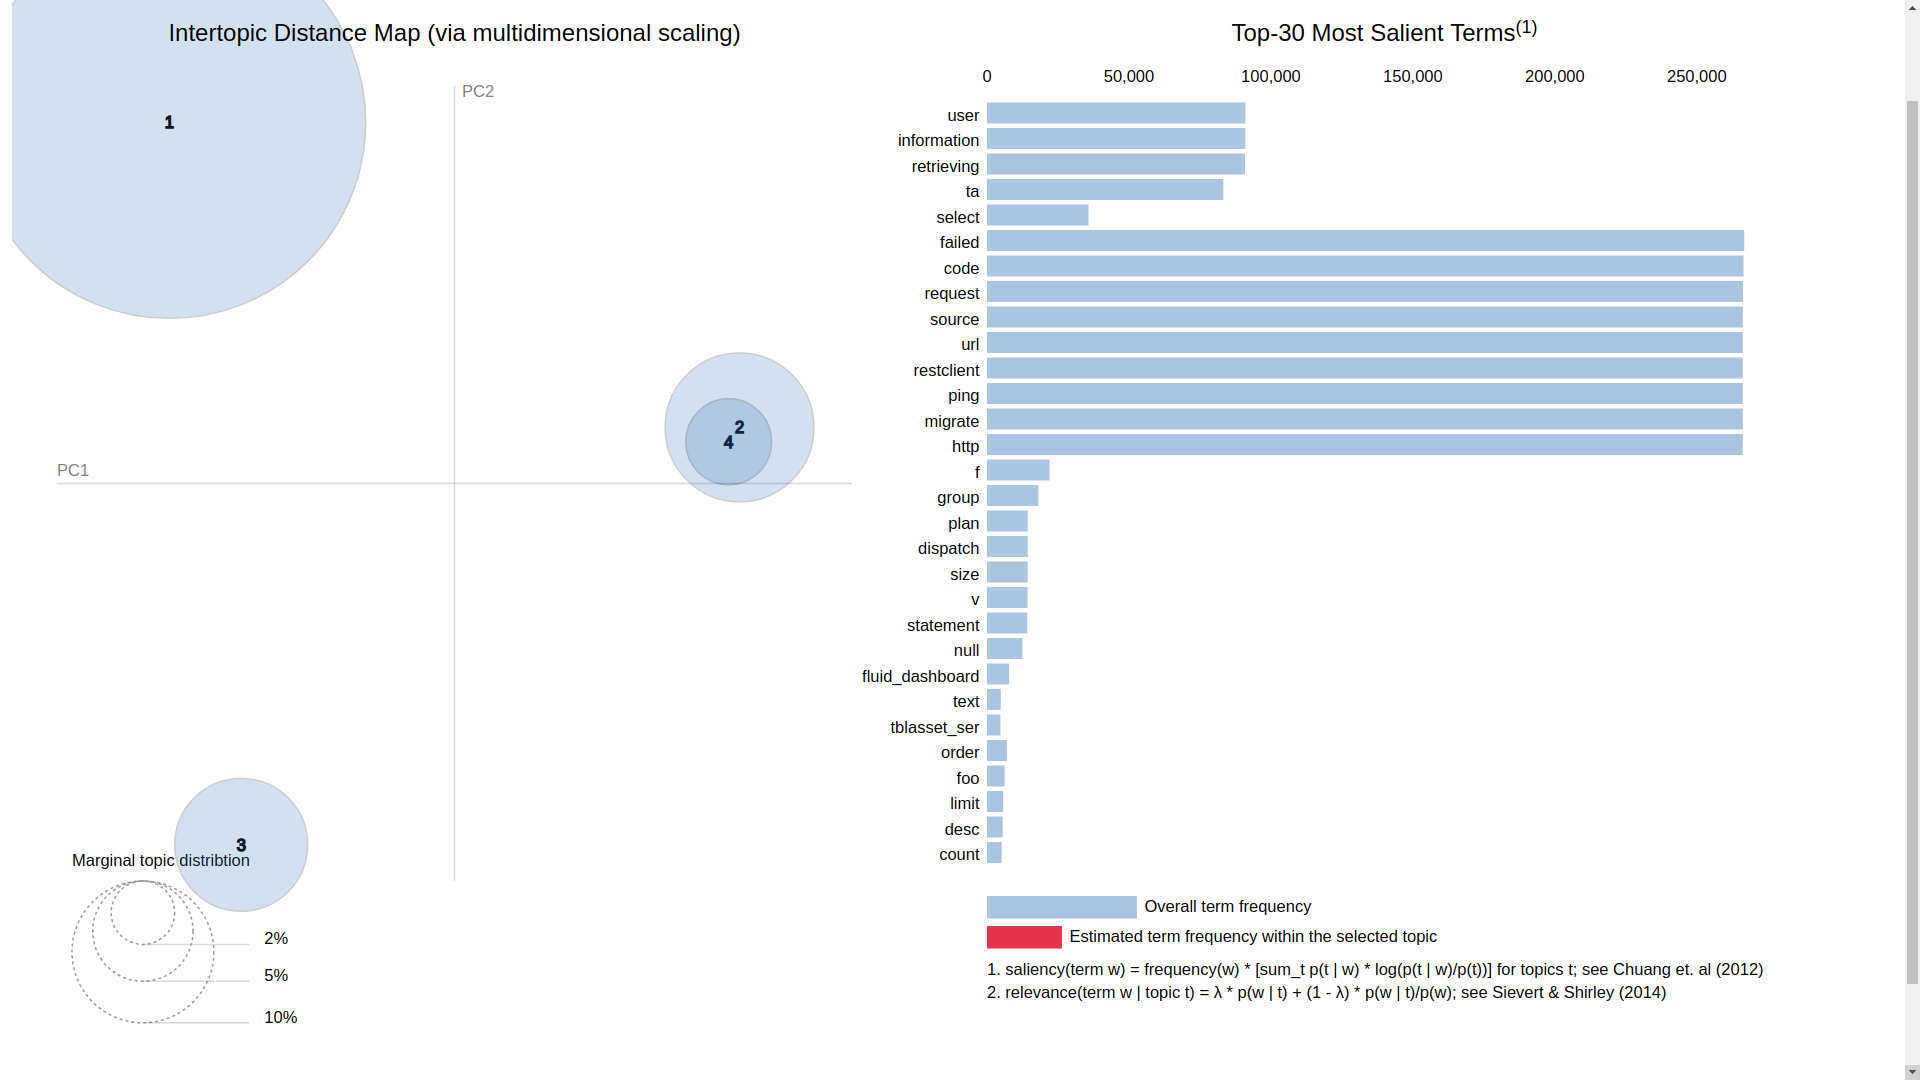
\includegraphics[width=15cm, height=8cm,trim=0 0 100px 0, clip=true]{figures/pyldavis/pyldavis_4.png}
    \caption{PyLdavis topic visualisation with 4 topics}
    \label{fig:pyldavis_4}
\end{figure}

  \begin{figure}[!h]
    \centering
    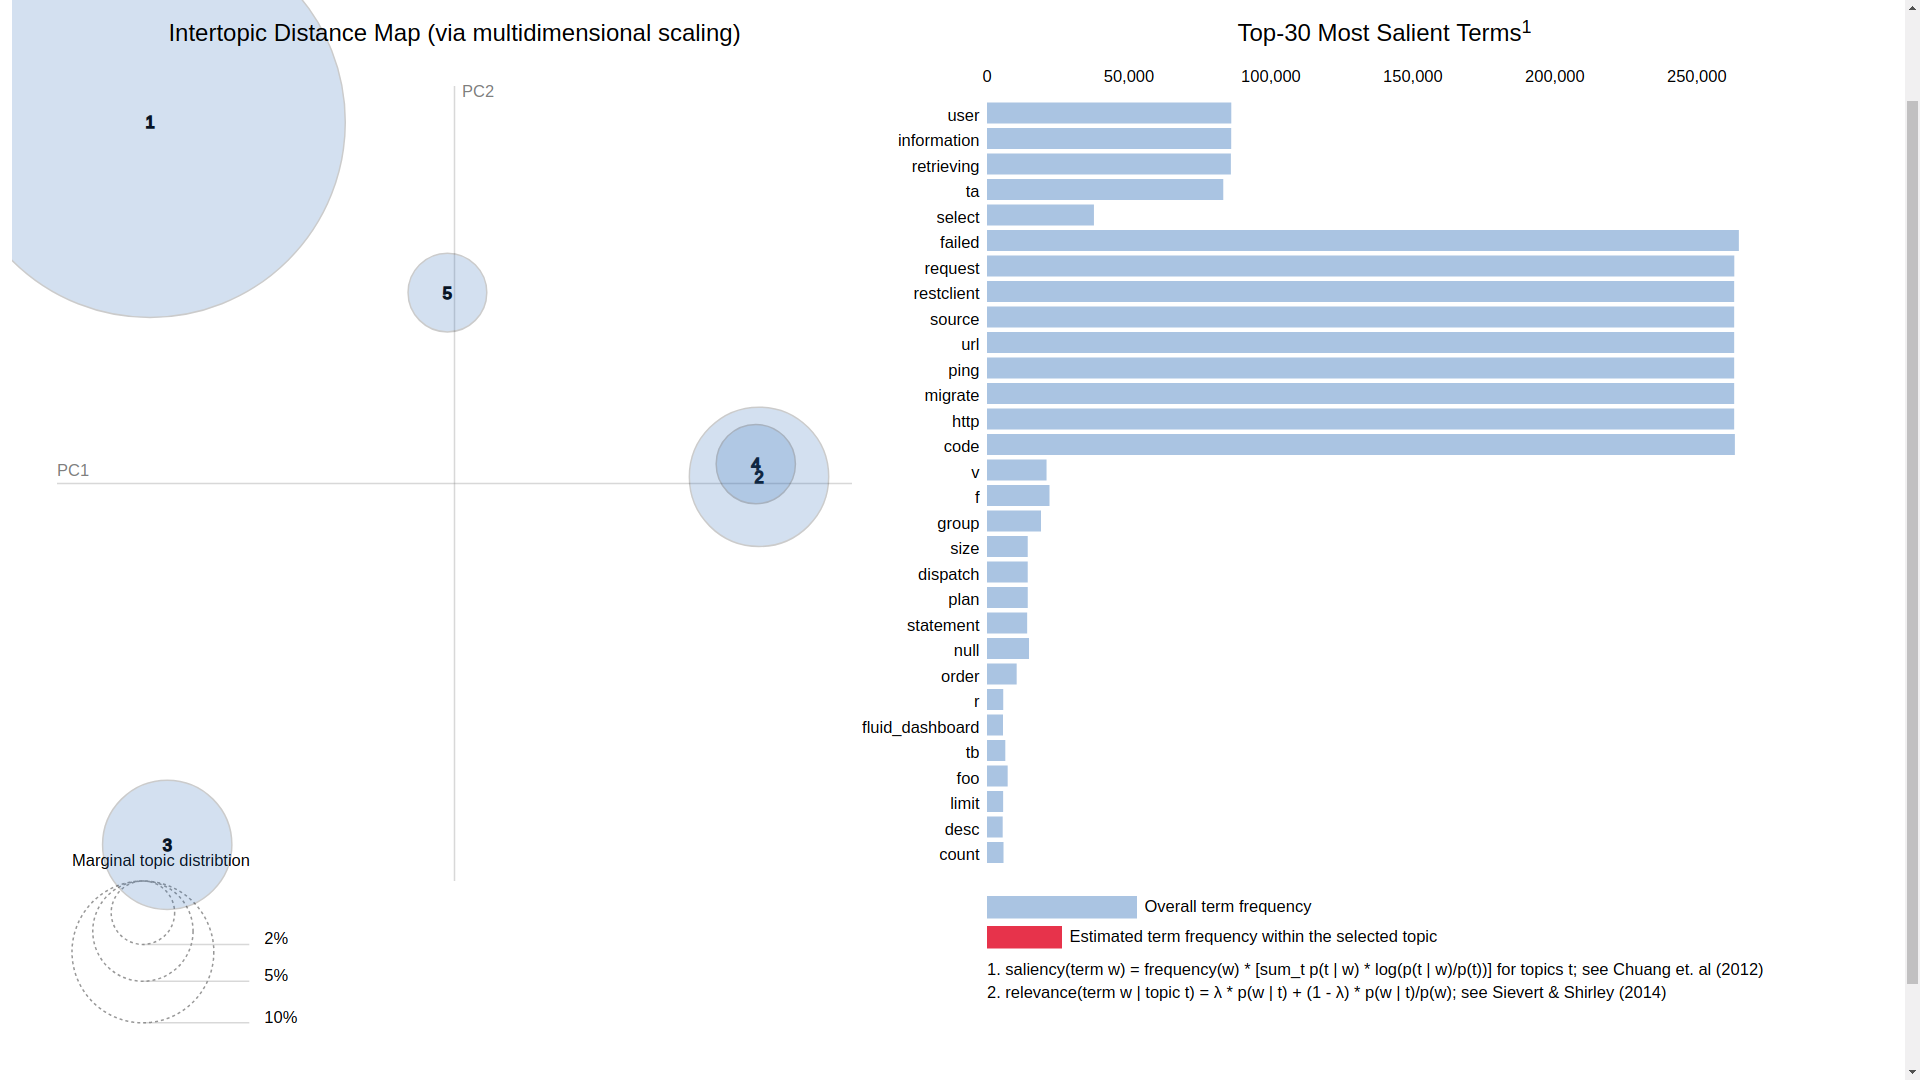
\includegraphics[width=15cm, height=8cm,trim=0 0 100px 0, clip=true]{figures/pyldavis/pyldavis_5.png}
    \caption{PyLdavis topic visualisation with 4 topics}
    \label{fig:appendices:pyldavis_5}
\end{figure}
 
 \begin{figure}[!h]
    \centering
    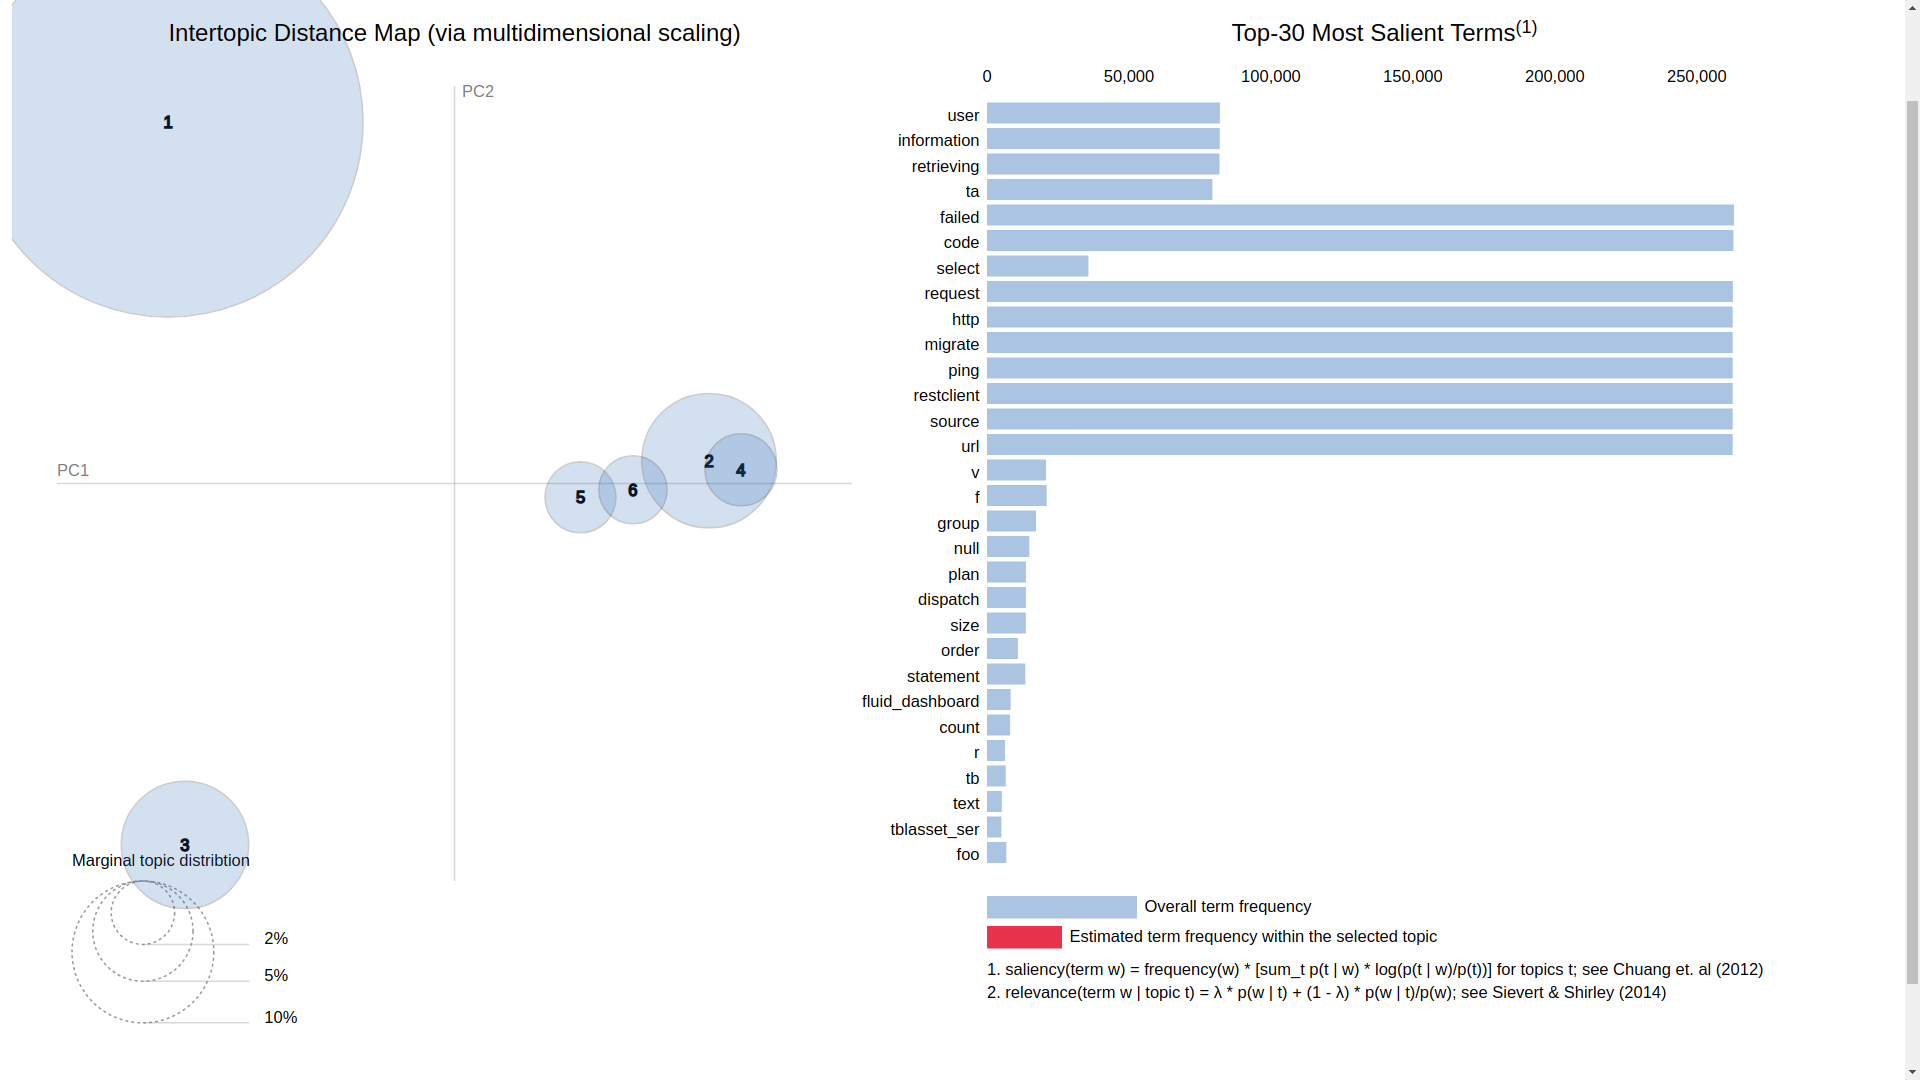
\includegraphics[width=15cm, height=8cm,trim=0 0 100px 0, clip=true]{figures/pyldavis/pyldavis_6.png}
    \caption{PyLdavis topic visualisation with 6 topics}
    \label{fig:pyldavis_6}
\end{figure}

 \begin{figure}[!h]
    \centering
    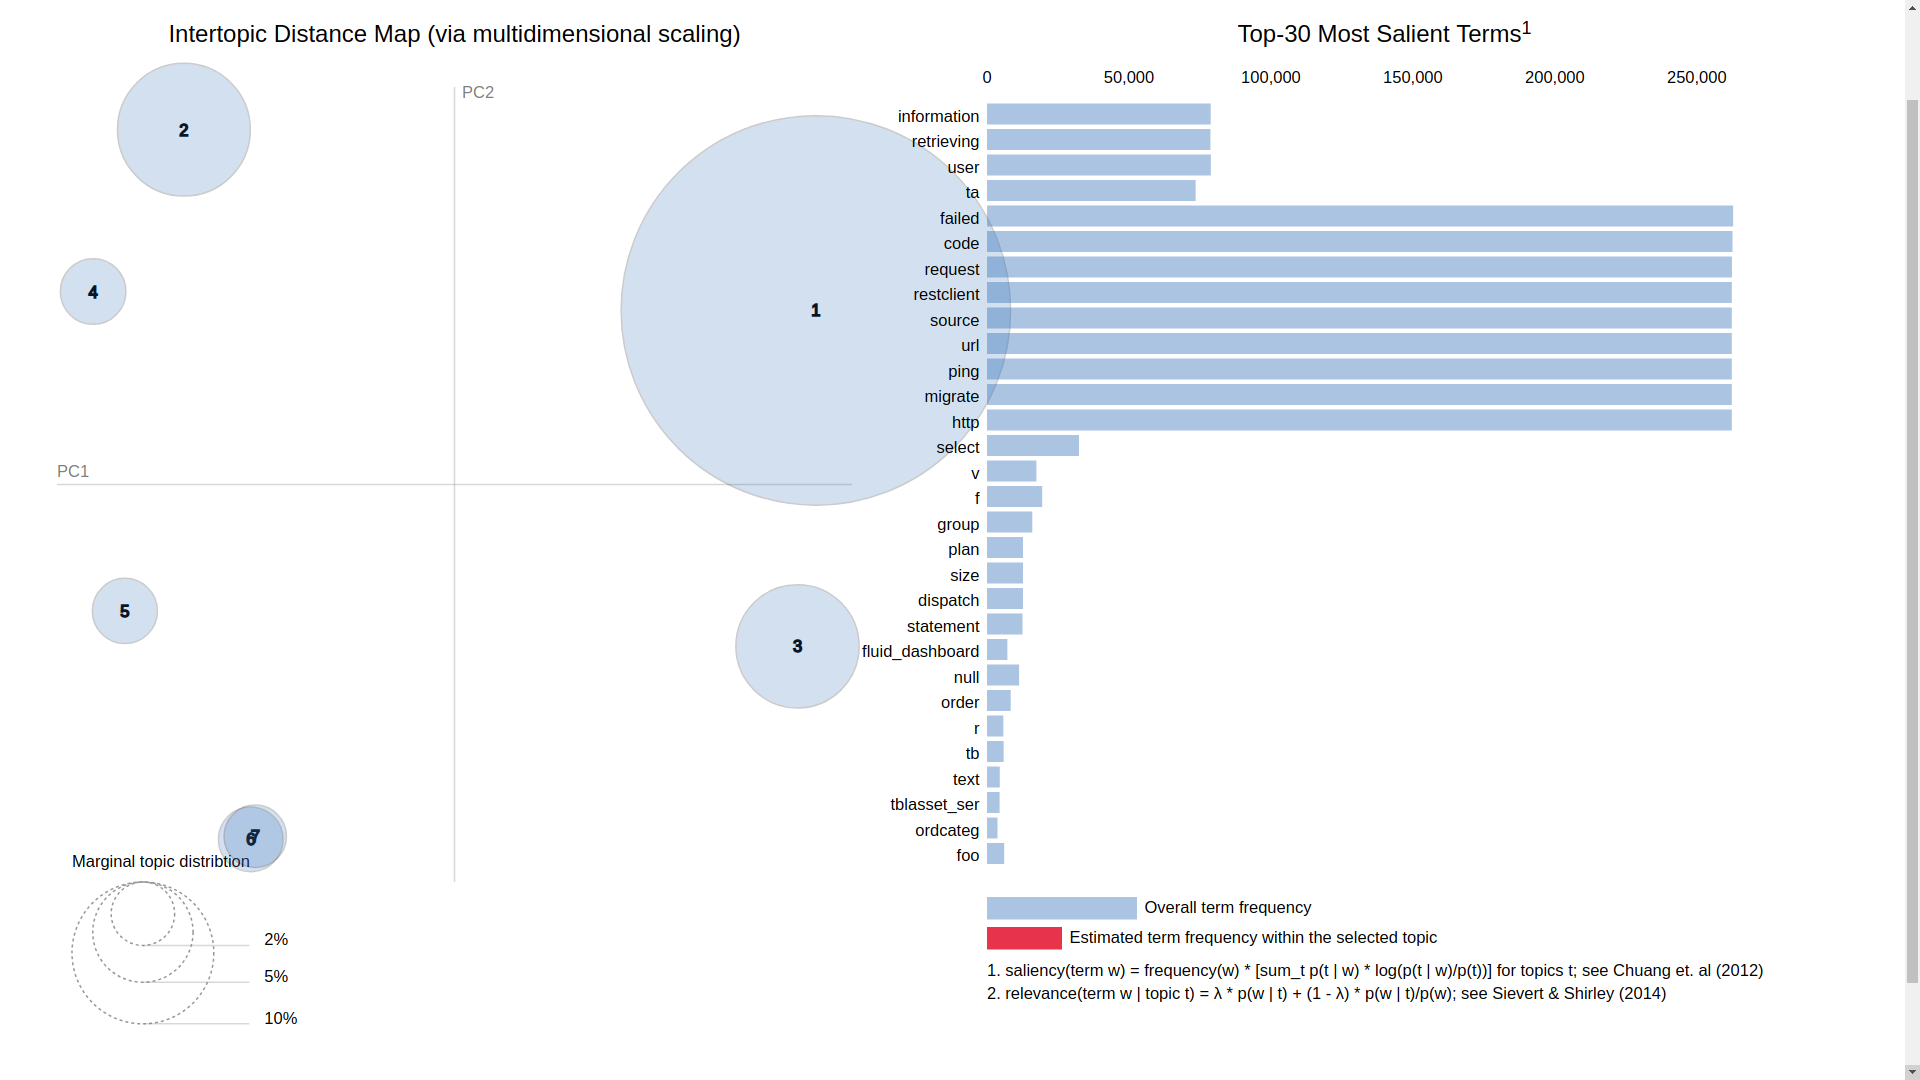
\includegraphics[width=15cm, height=8cm,trim=0 0 100px 0, clip=true]{figures/pyldavis/pyldavis_7.png}
    \caption{PyLdavis topic visualisation with 7 topics}
    \label{fig:pyldavis_7}
\end{figure}

 \begin{figure}[h]
    \centering
    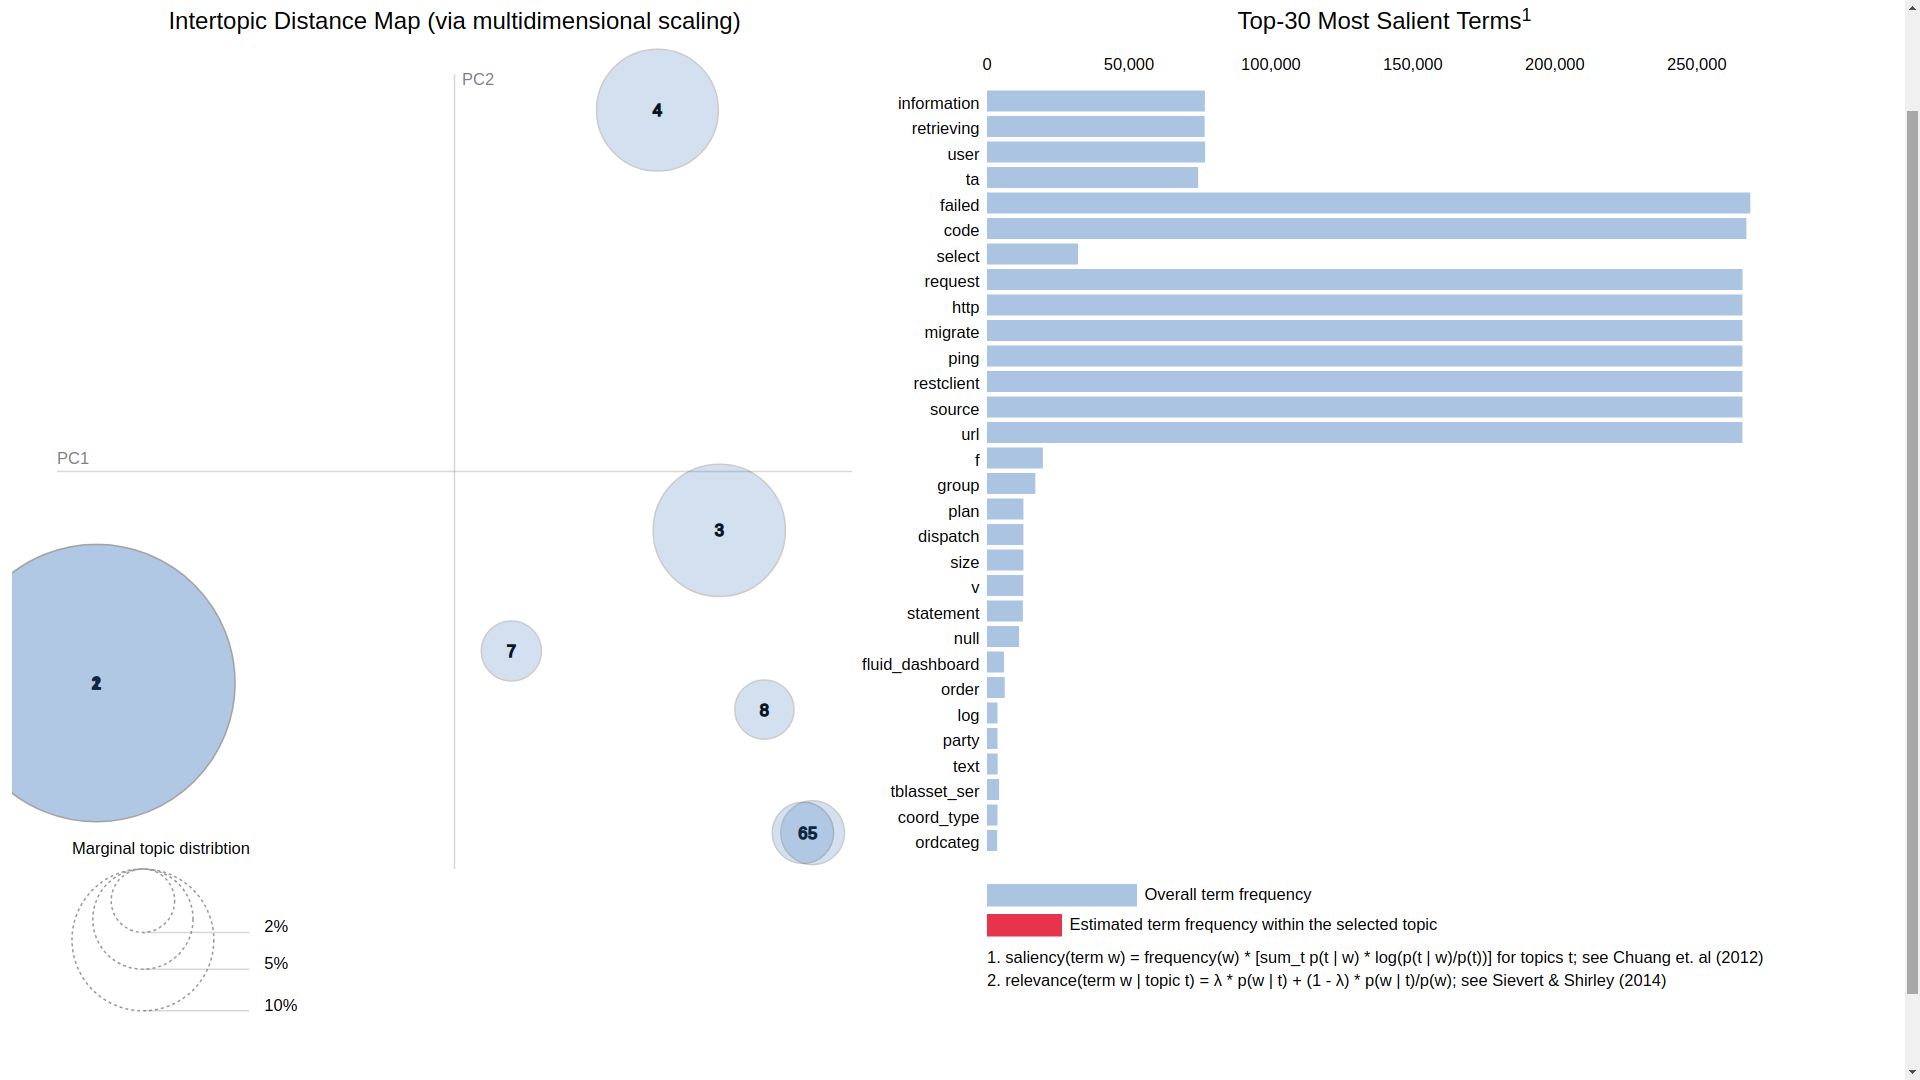
\includegraphics[width=15cm, height=8cm,trim=0 0 100px 0, clip=true]{figures/pyldavis/pyldavis_8.png}
    \caption{PyLdavis topic visualisation with 8 topics}
    \label{fig:pyldavis_8}
\end{figure}

 \begin{figure}[!h]
    \centering
    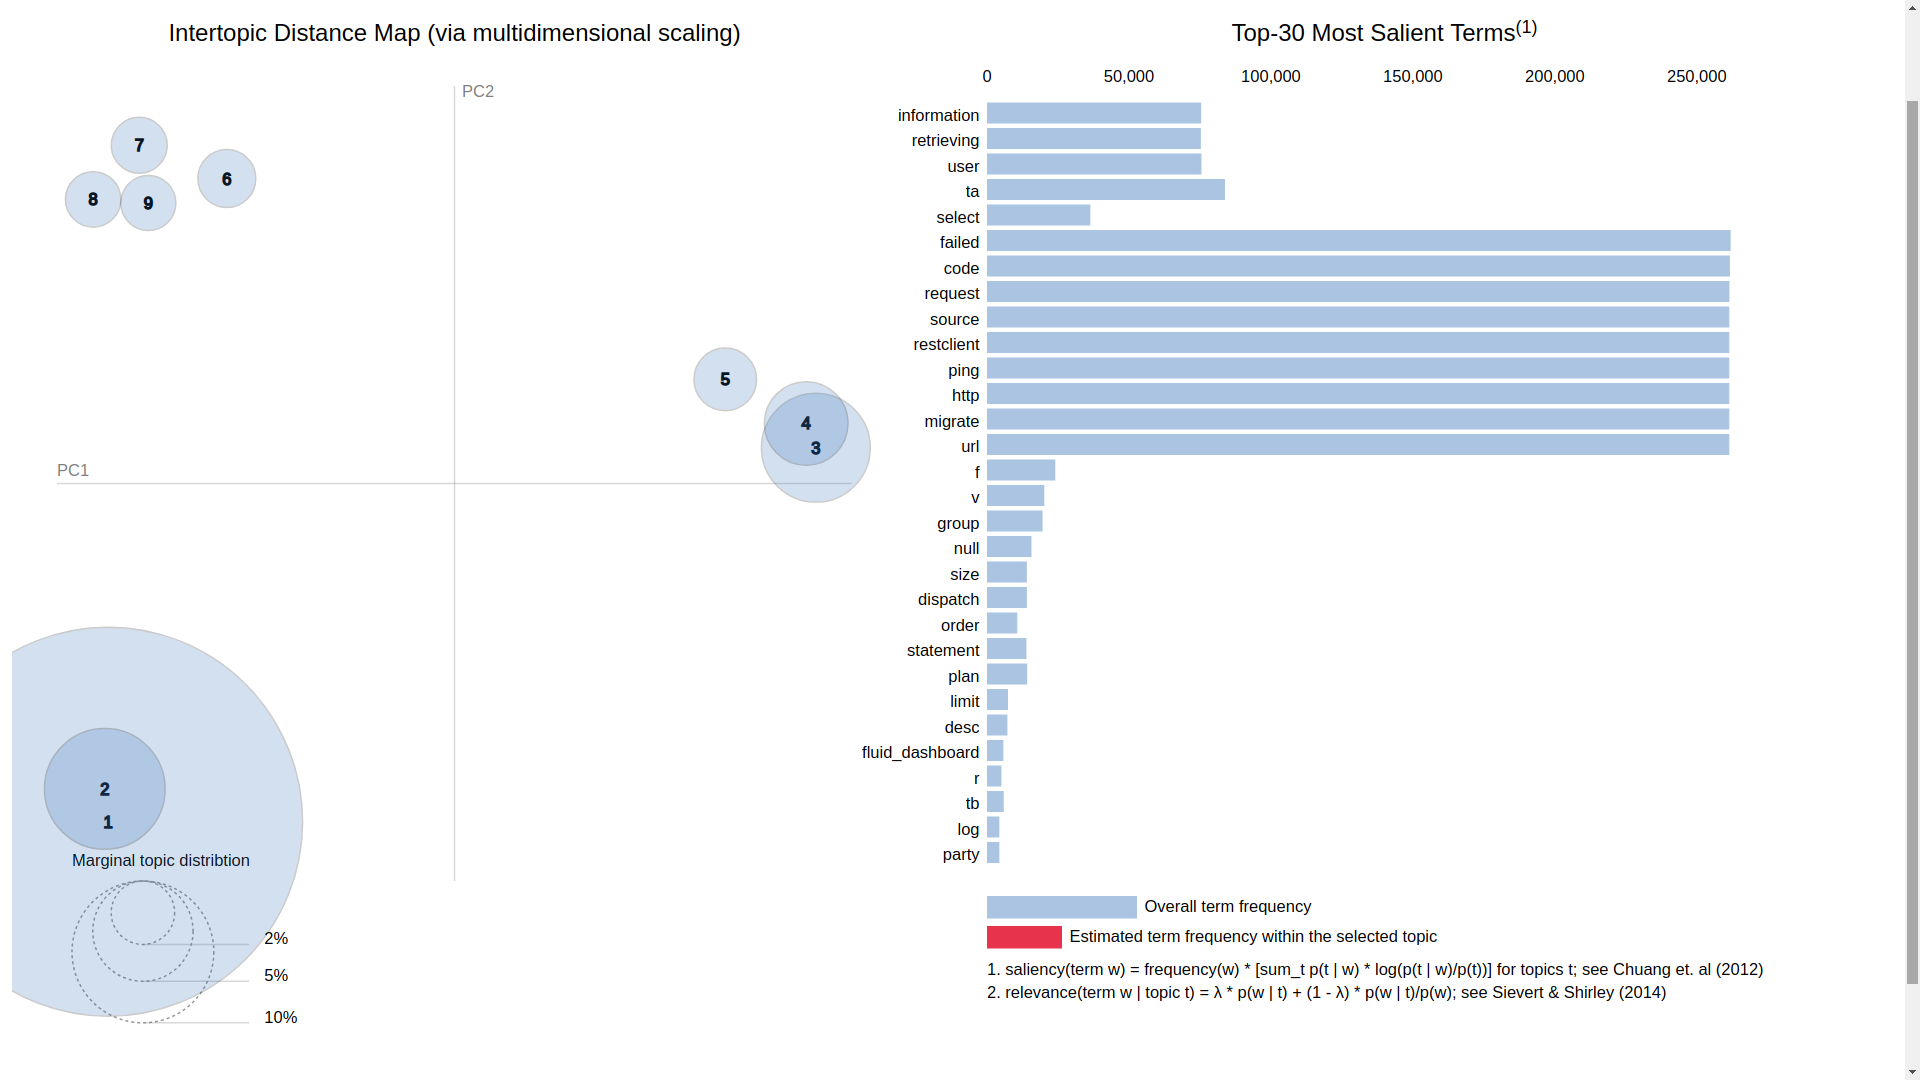
\includegraphics[width=15cm, height=8cm,trim=0 0 100px 0, clip=true]{figures/pyldavis/pyldavis_9.png}
    \caption{PyLdavis topic visualisation with 9 topics}
    \label{fig:pyldavis_9}
\end{figure}

 \begin{figure}[!h]
    \centering
    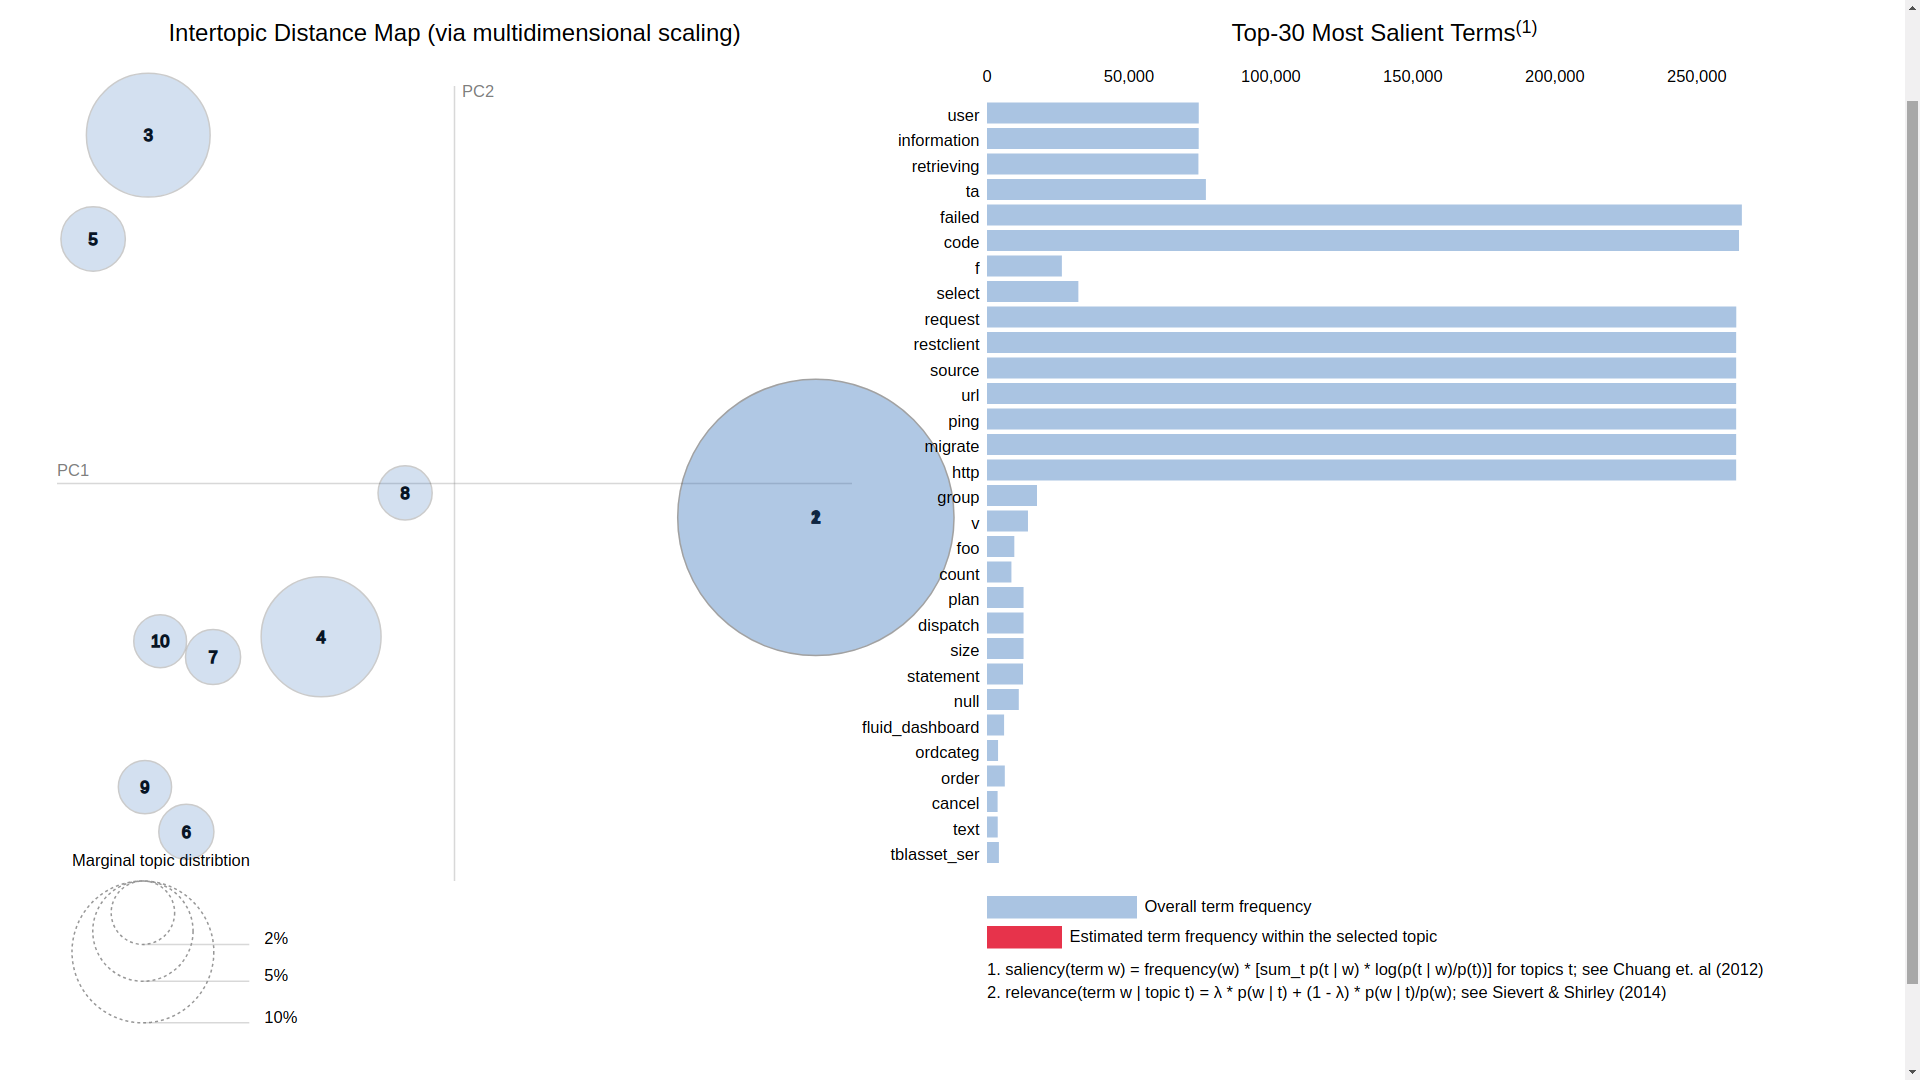
\includegraphics[width=15cm, height=8cm,trim=0 0 100px 0, clip=true]{figures/pyldavis/pyldavis_10.png}
    \caption{PyLdavis topic visualisation with 10 topics}
    \label{fig:appendices:pyldavis_10}
\end{figure}

 \begin{figure}[!h]
    \centering
    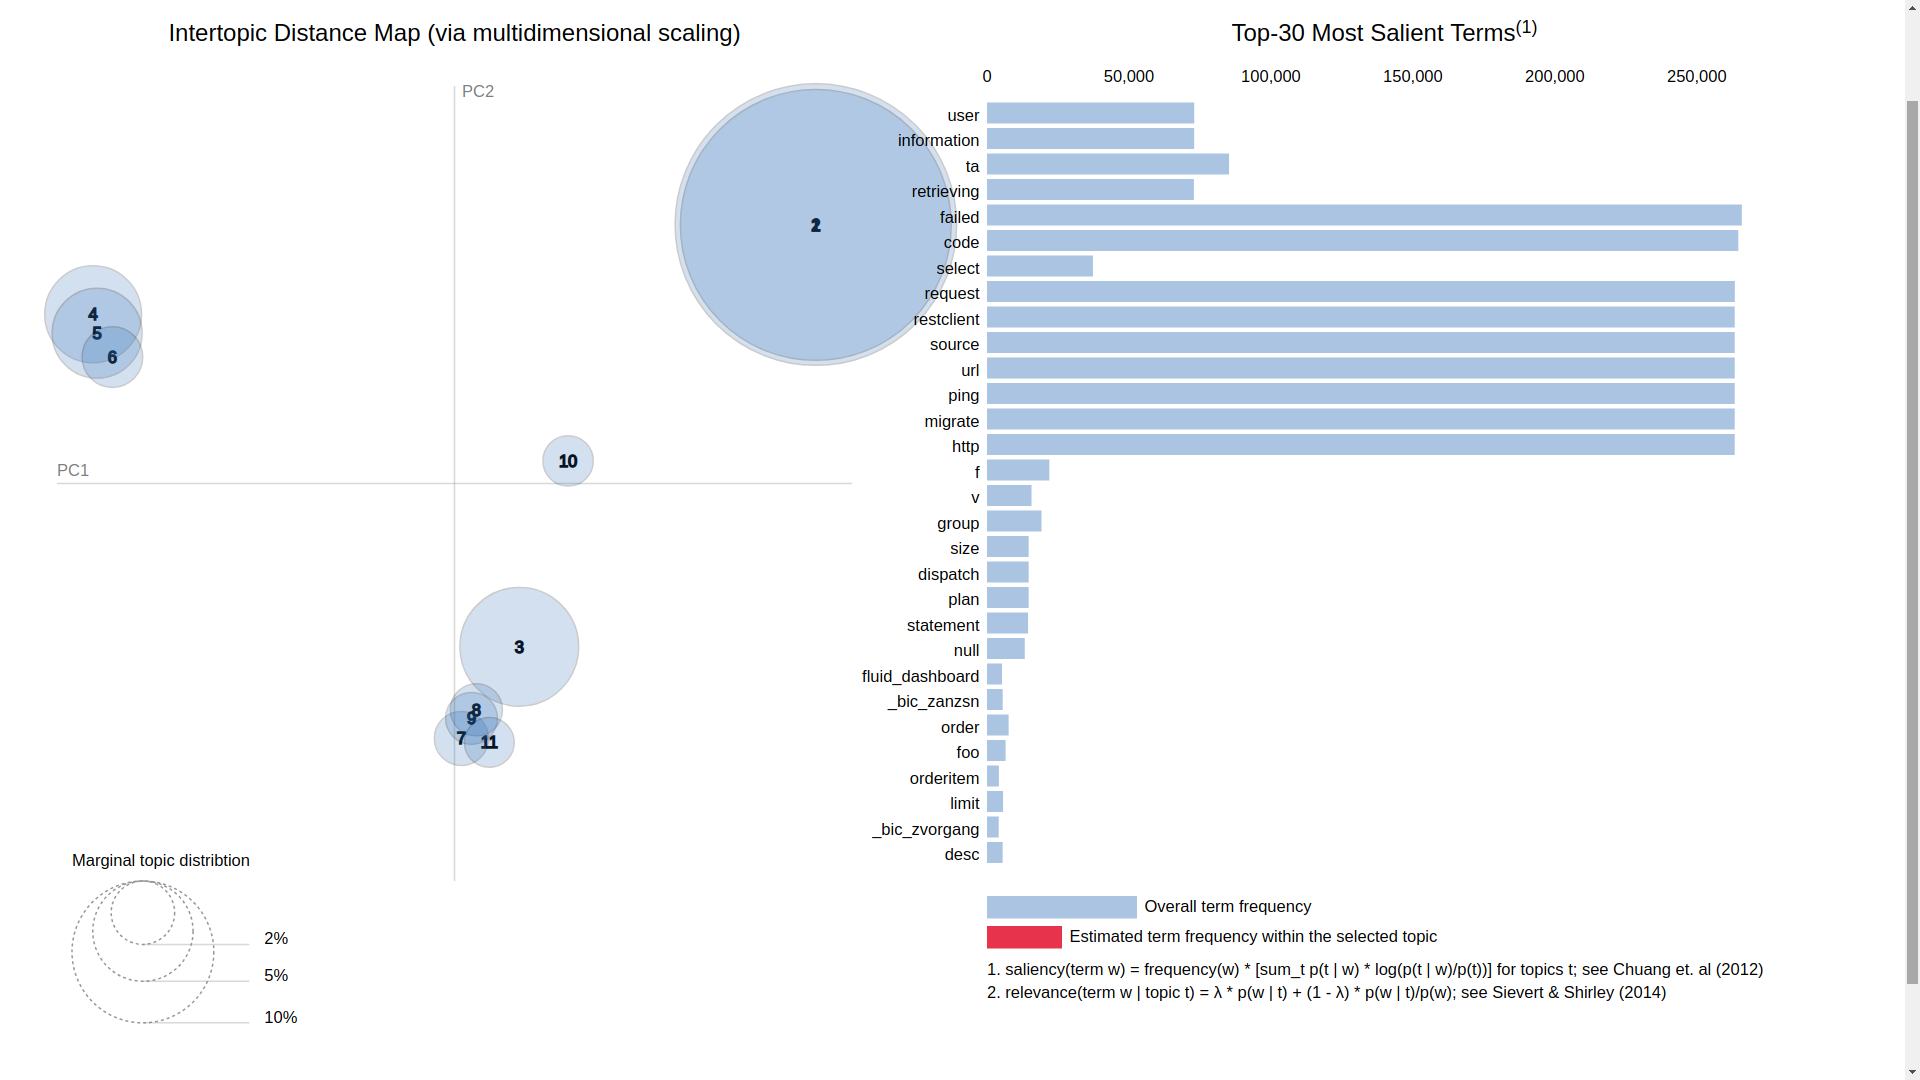
\includegraphics[width=15cm, height=8cm,trim=0 0 100px 0, clip=true]{figures/pyldavis/pyldavis_11.png}
    \caption{PyLdavis topic visualisation with 11 topics}
    \label{fig:pyldavis_11}
\end{figure}

 \begin{figure}[!h]
    \centering
    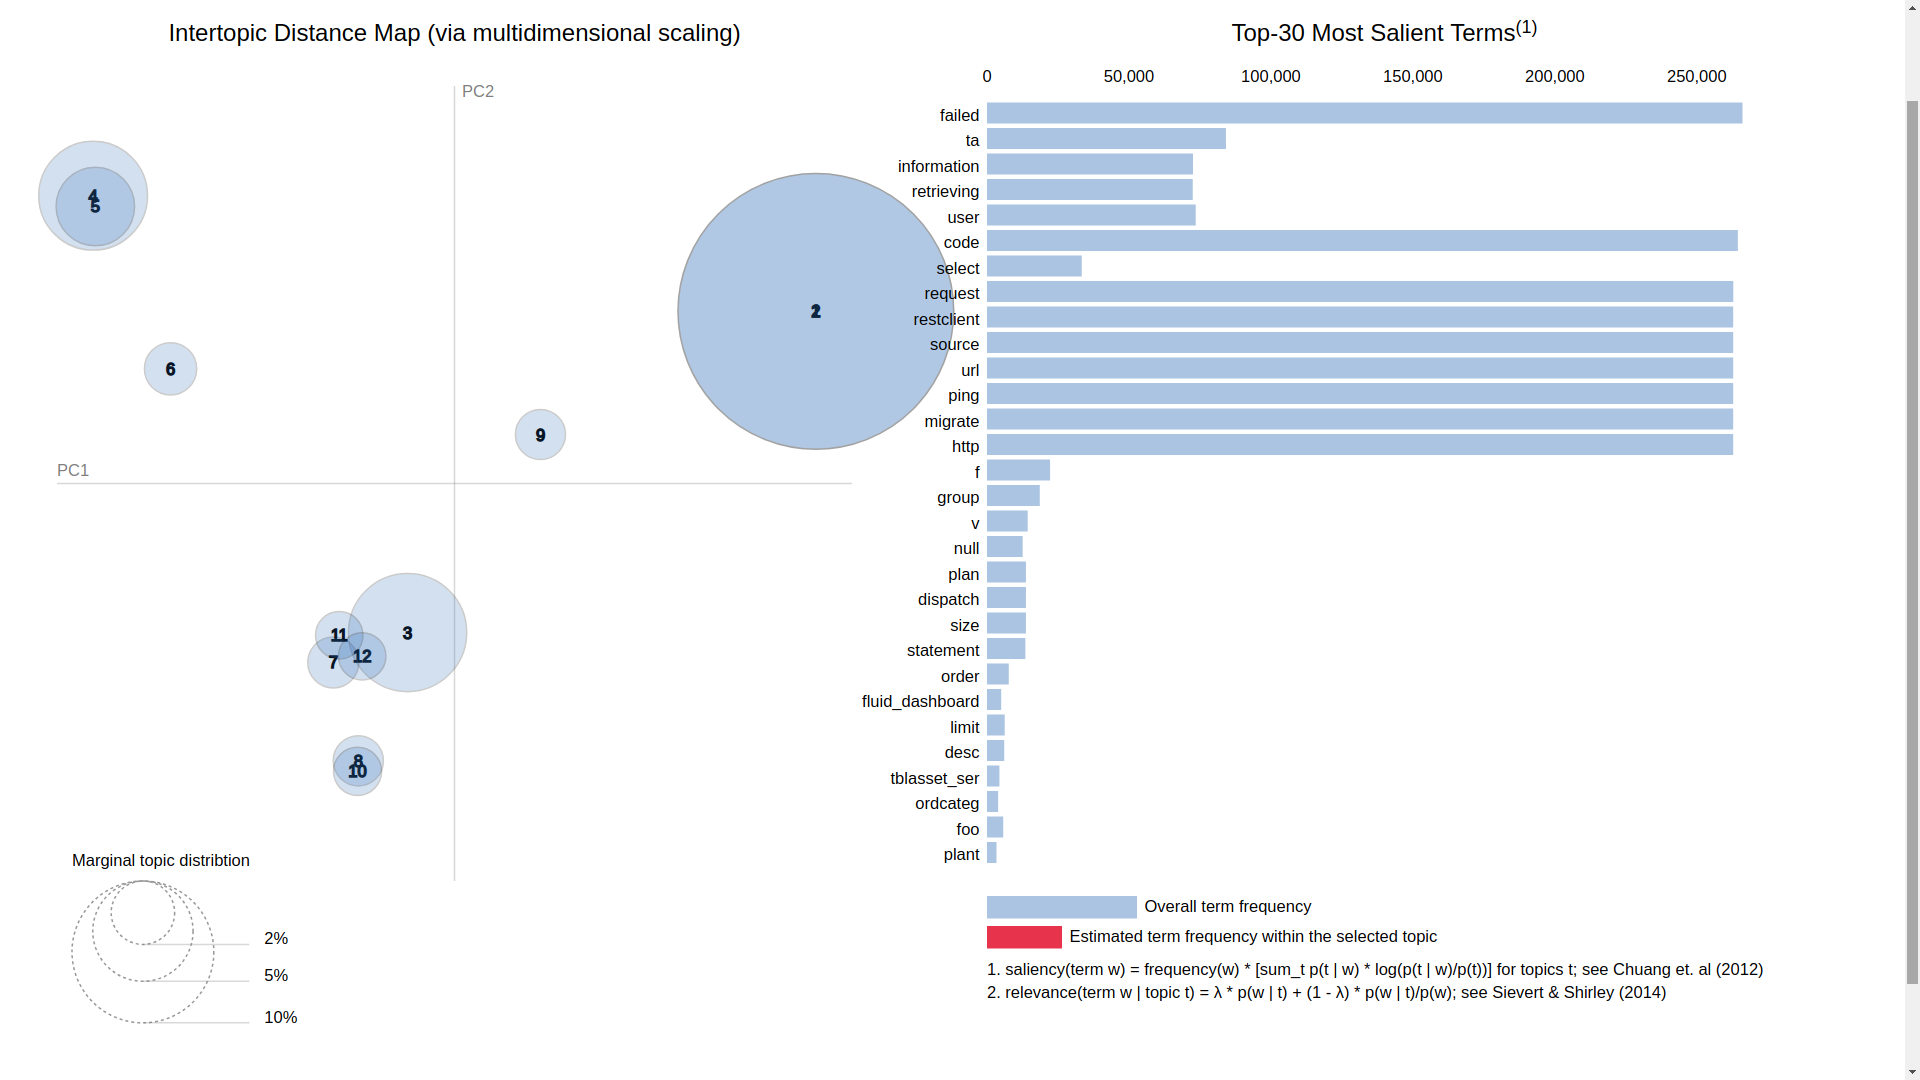
\includegraphics[width=15cm, height=8cm,trim=0 0 100px 0, clip=true]{figures/pyldavis/pyldavis_12.png}
    \caption{PyLdavis topic visualisation with 12 topics}
    \label{fig:pyldavis_12}
\end{figure}

 \begin{figure}[!h]
    \centering
    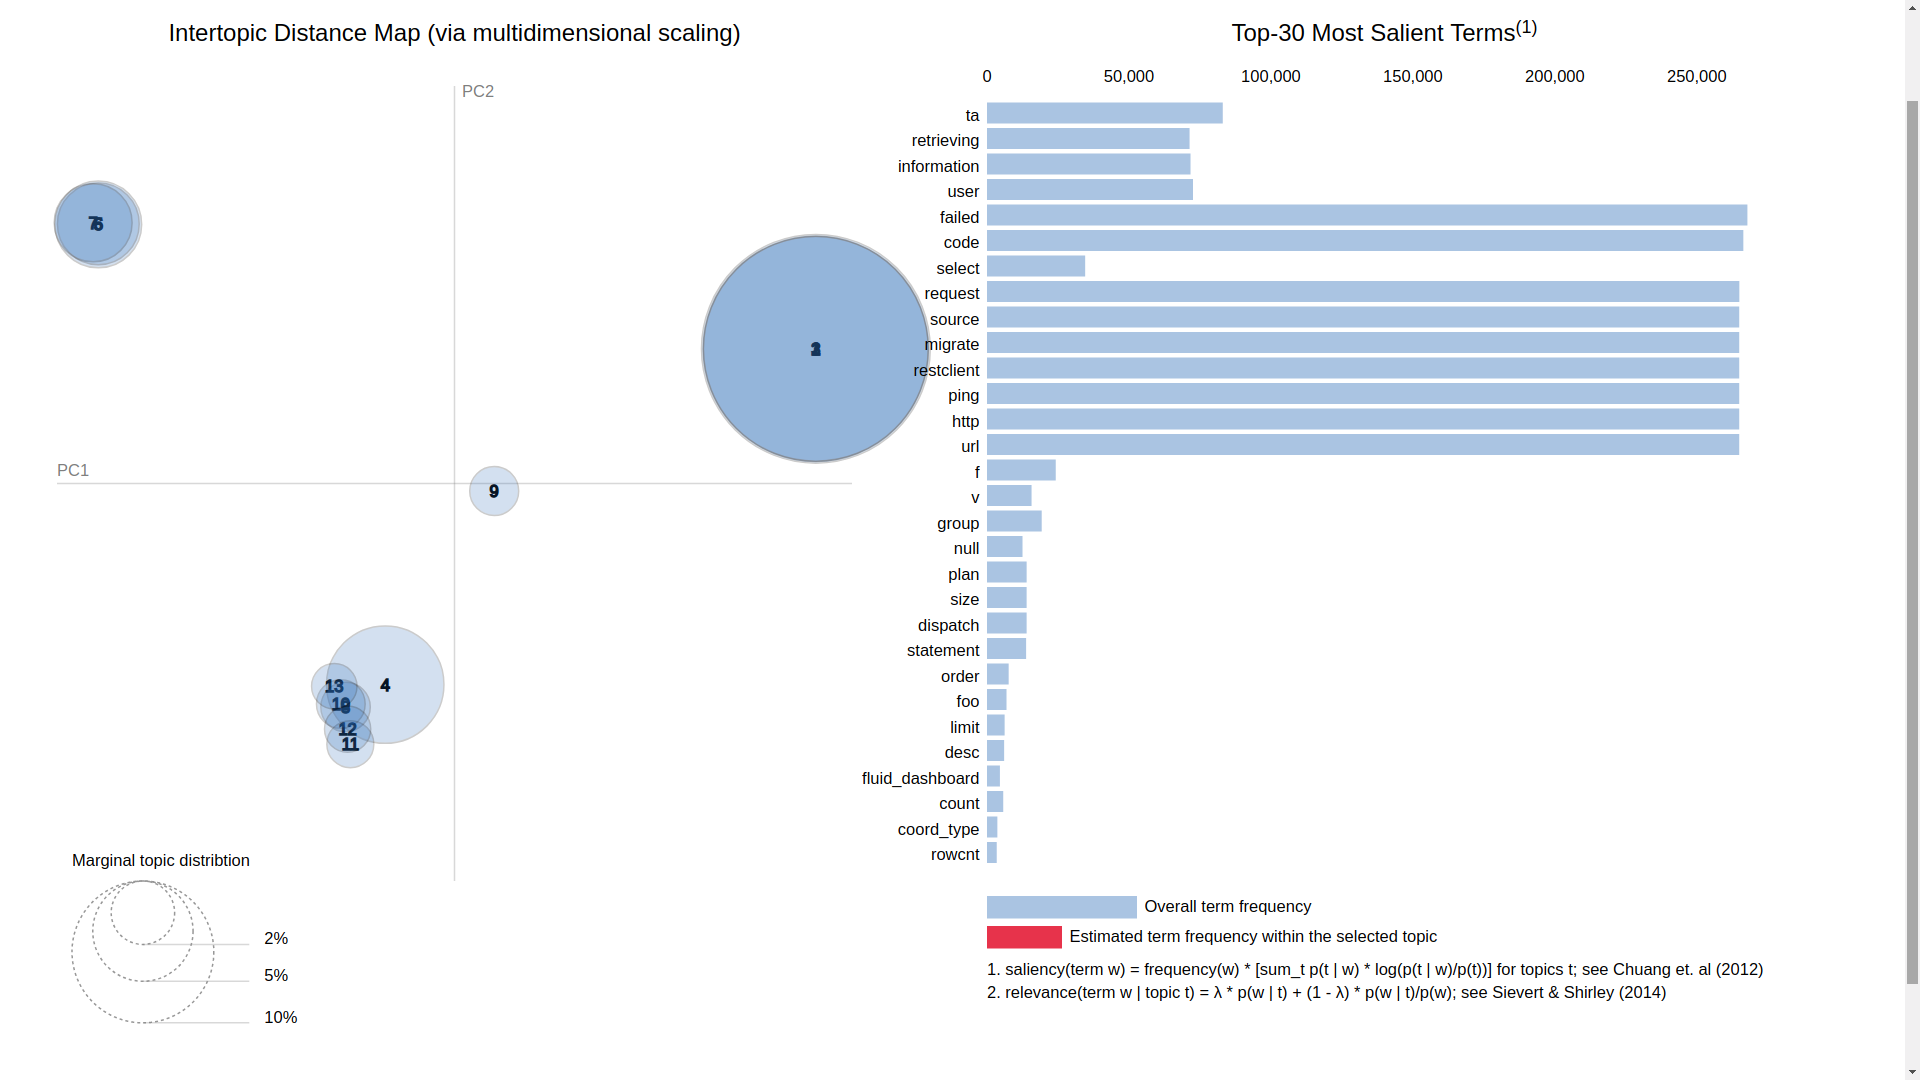
\includegraphics[width=15cm, height=8cm,trim=0 0 100px 0, clip=true]{figures/pyldavis/pyldavis_13.png}
    \caption{PyLdavis topic visualisation with 13 topics}
    \label{fig:pyldavis_13}
\end{figure}

 \begin{figure}[!h]
    \centering
    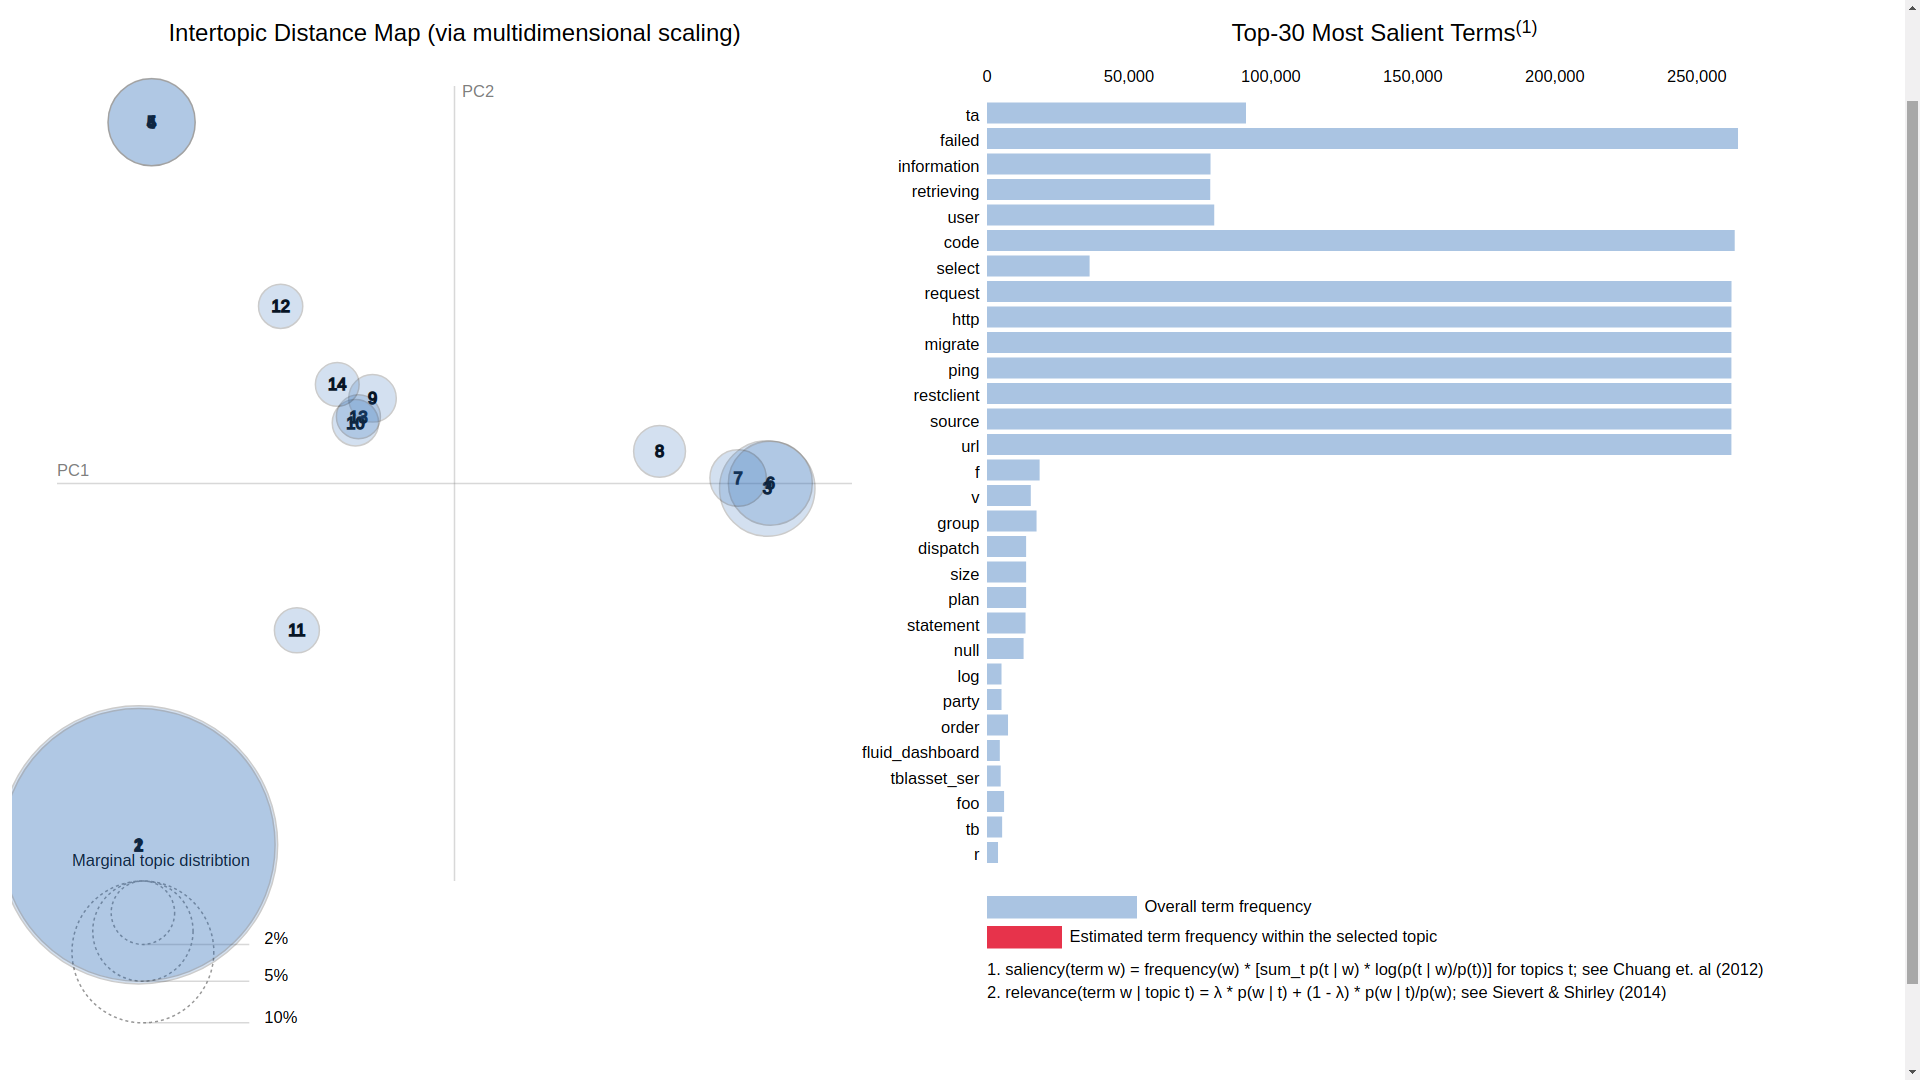
\includegraphics[width=15cm, height=8cm,trim=0 0 100px 0, clip=true]{figures/pyldavis/pyldavis_14.png}
    \caption{PyLdavis topic visualisation with 14 topics}
    \label{fig:pyldavis_14}
\end{figure}

 \begin{figure}[!h]
    \centering
    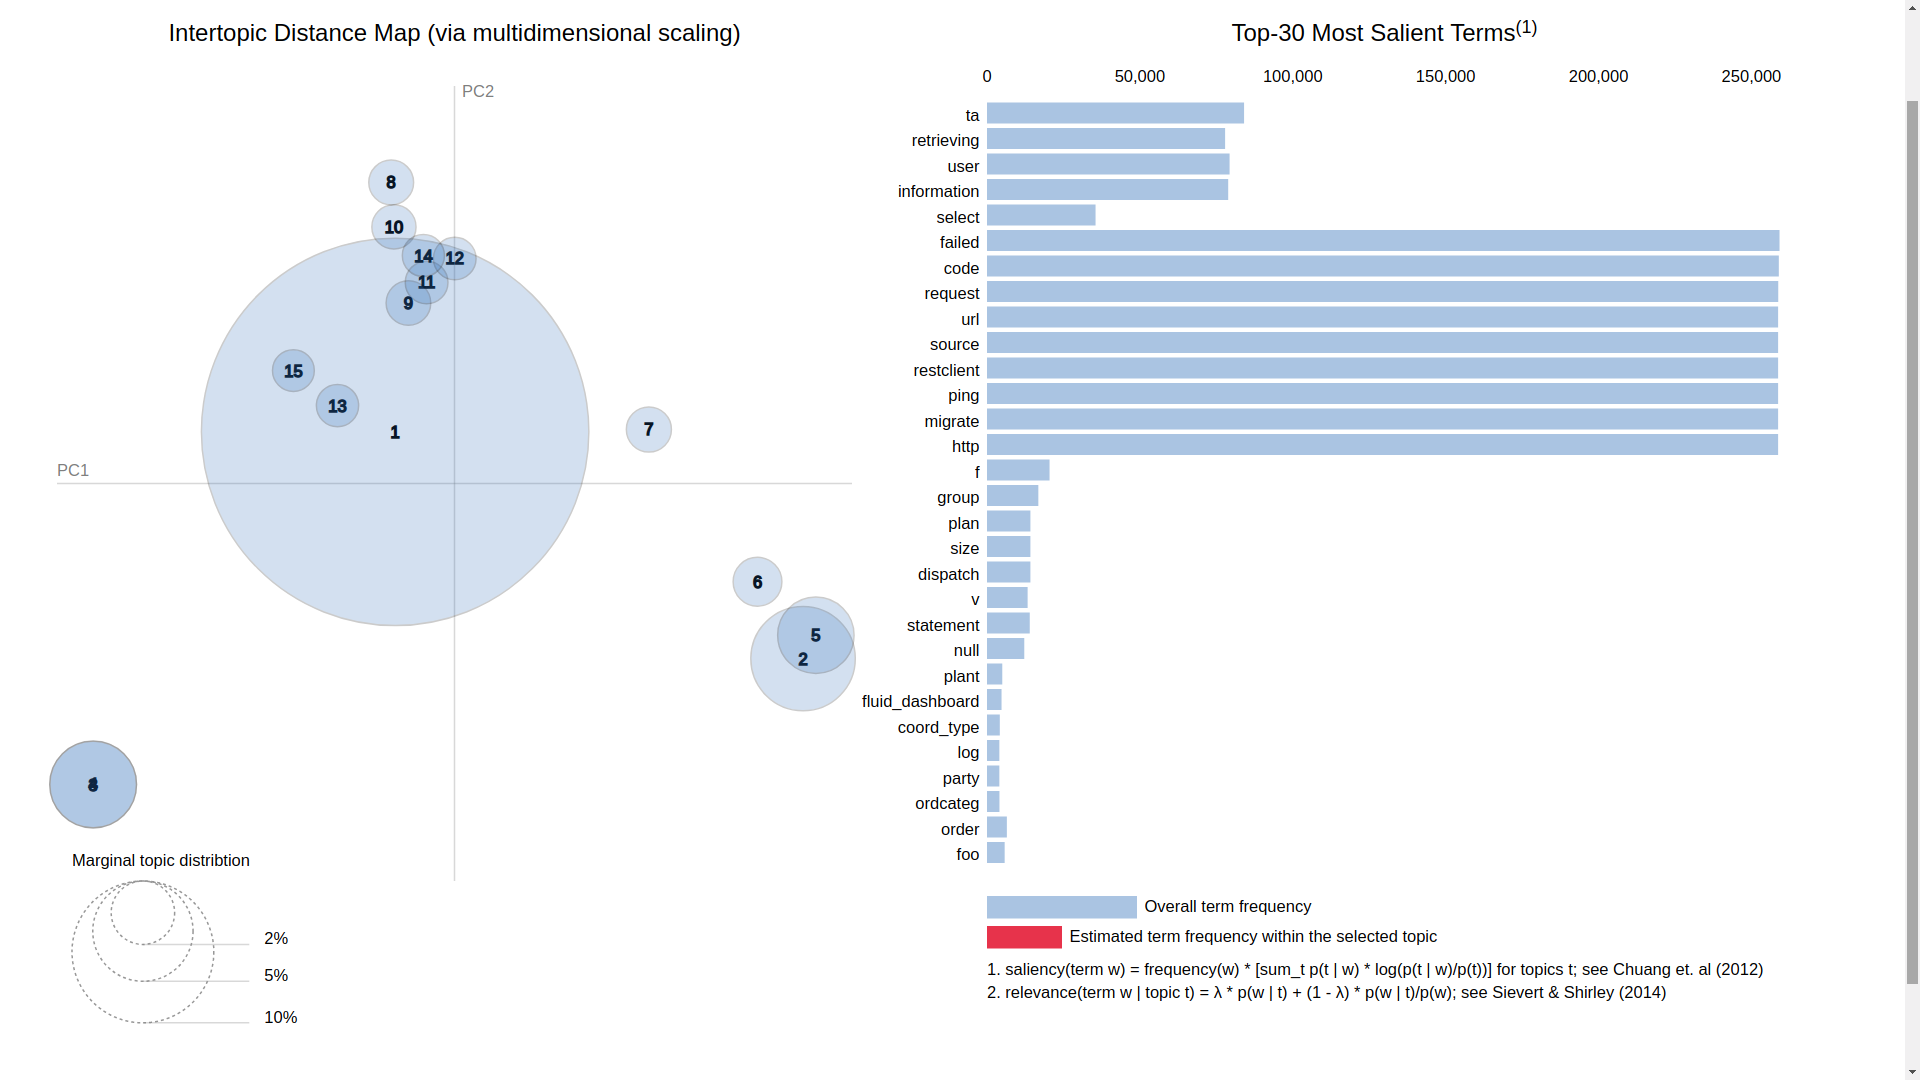
\includegraphics[width=15cm, height=8cm,trim=0 0 100px 0, clip=true]{figures/pyldavis/pyldavis_15.png}
    \caption{PyLdavis topic visualisation with 15 topics}
    \label{fig:pyldavis_15}
\end{figure}

 \begin{figure}[!h]
    \centering
    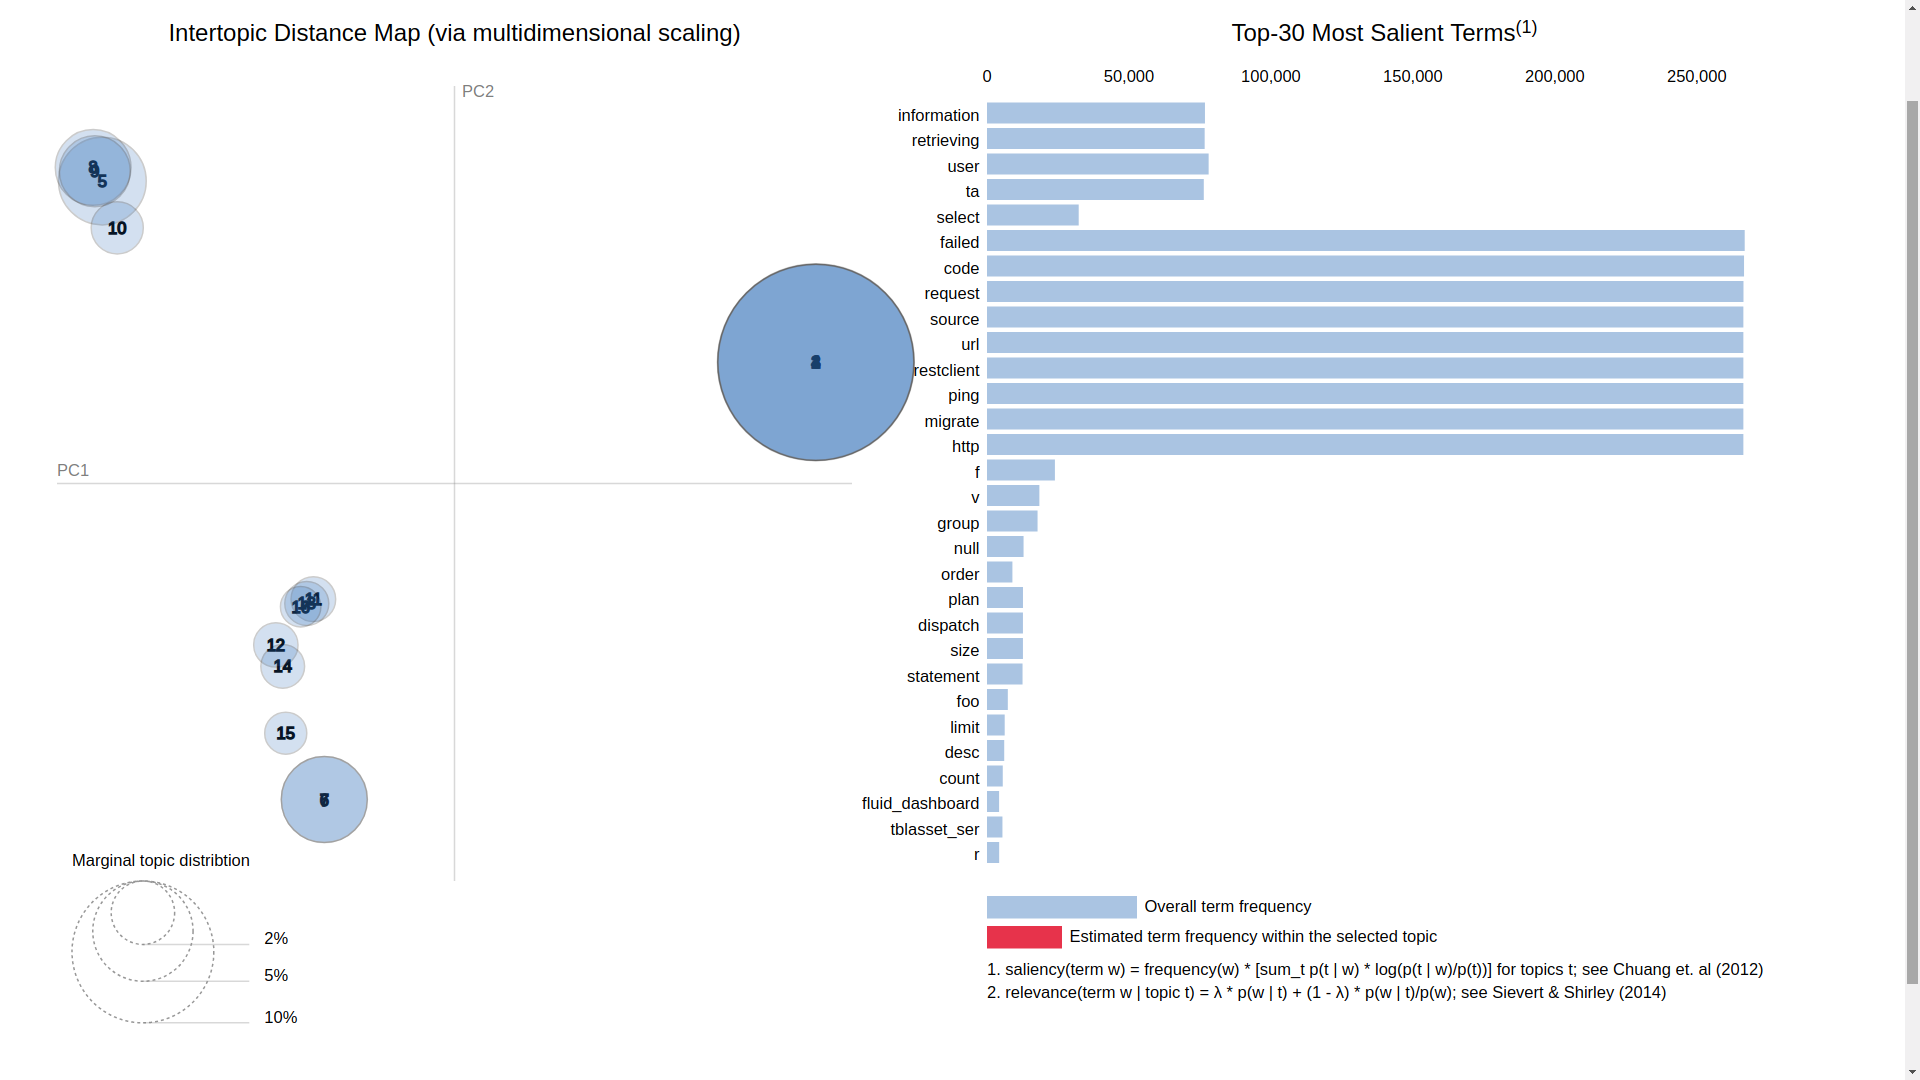
\includegraphics[width=15cm, height=8cm,trim=0 0 100px 0, clip=true]{figures/pyldavis/pyldavis_16.png}
    \caption{PyLdavis topic visualisation with 16 topics}
    \label{fig:pyldavis_16}
\end{figure}

 \begin{figure}[!h]
    \centering
    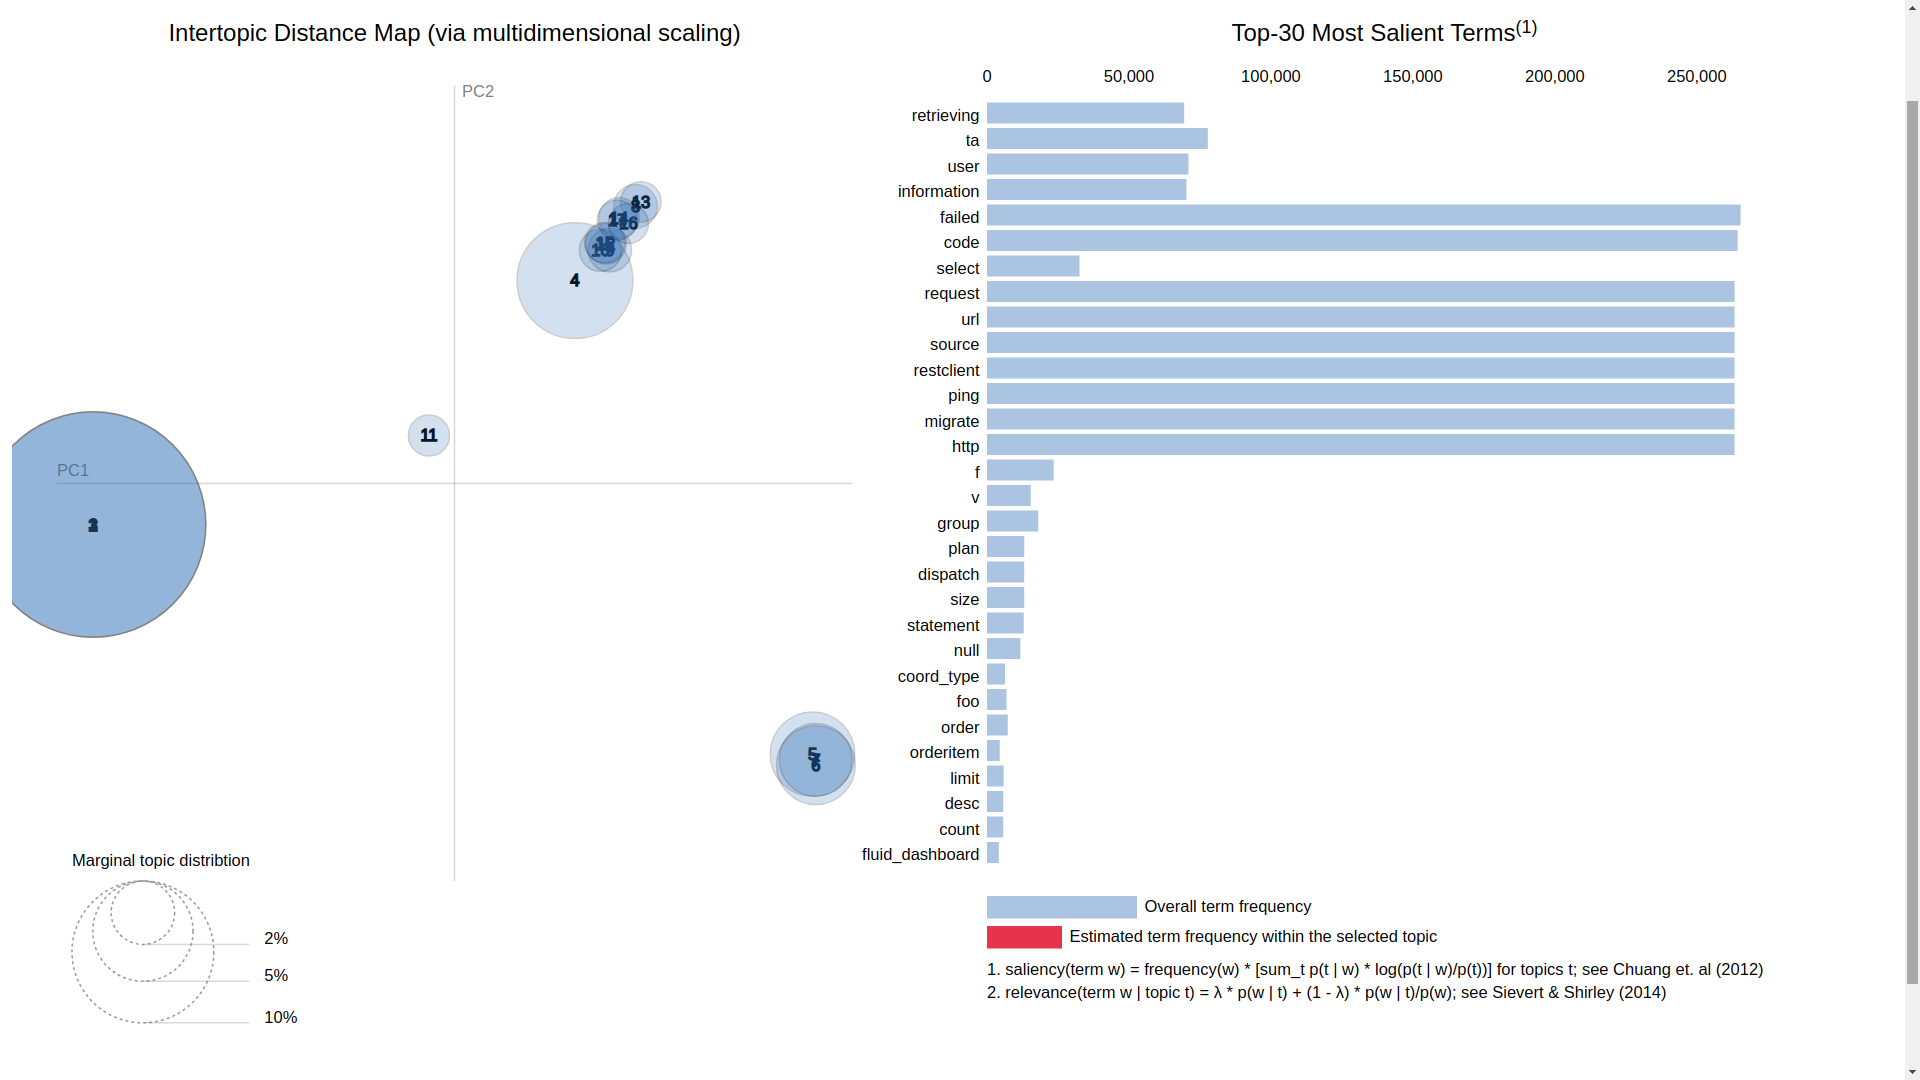
\includegraphics[width=15cm, height=8cm,trim=0 0 100px 0, clip=true]{figures/pyldavis/pyldavis_17.png}
    \caption{PyLdavis topic visualisation with 17 topics}
    \label{fig:pyldavis_17}
\end{figure}

 \begin{figure}[!h]
    \centering
    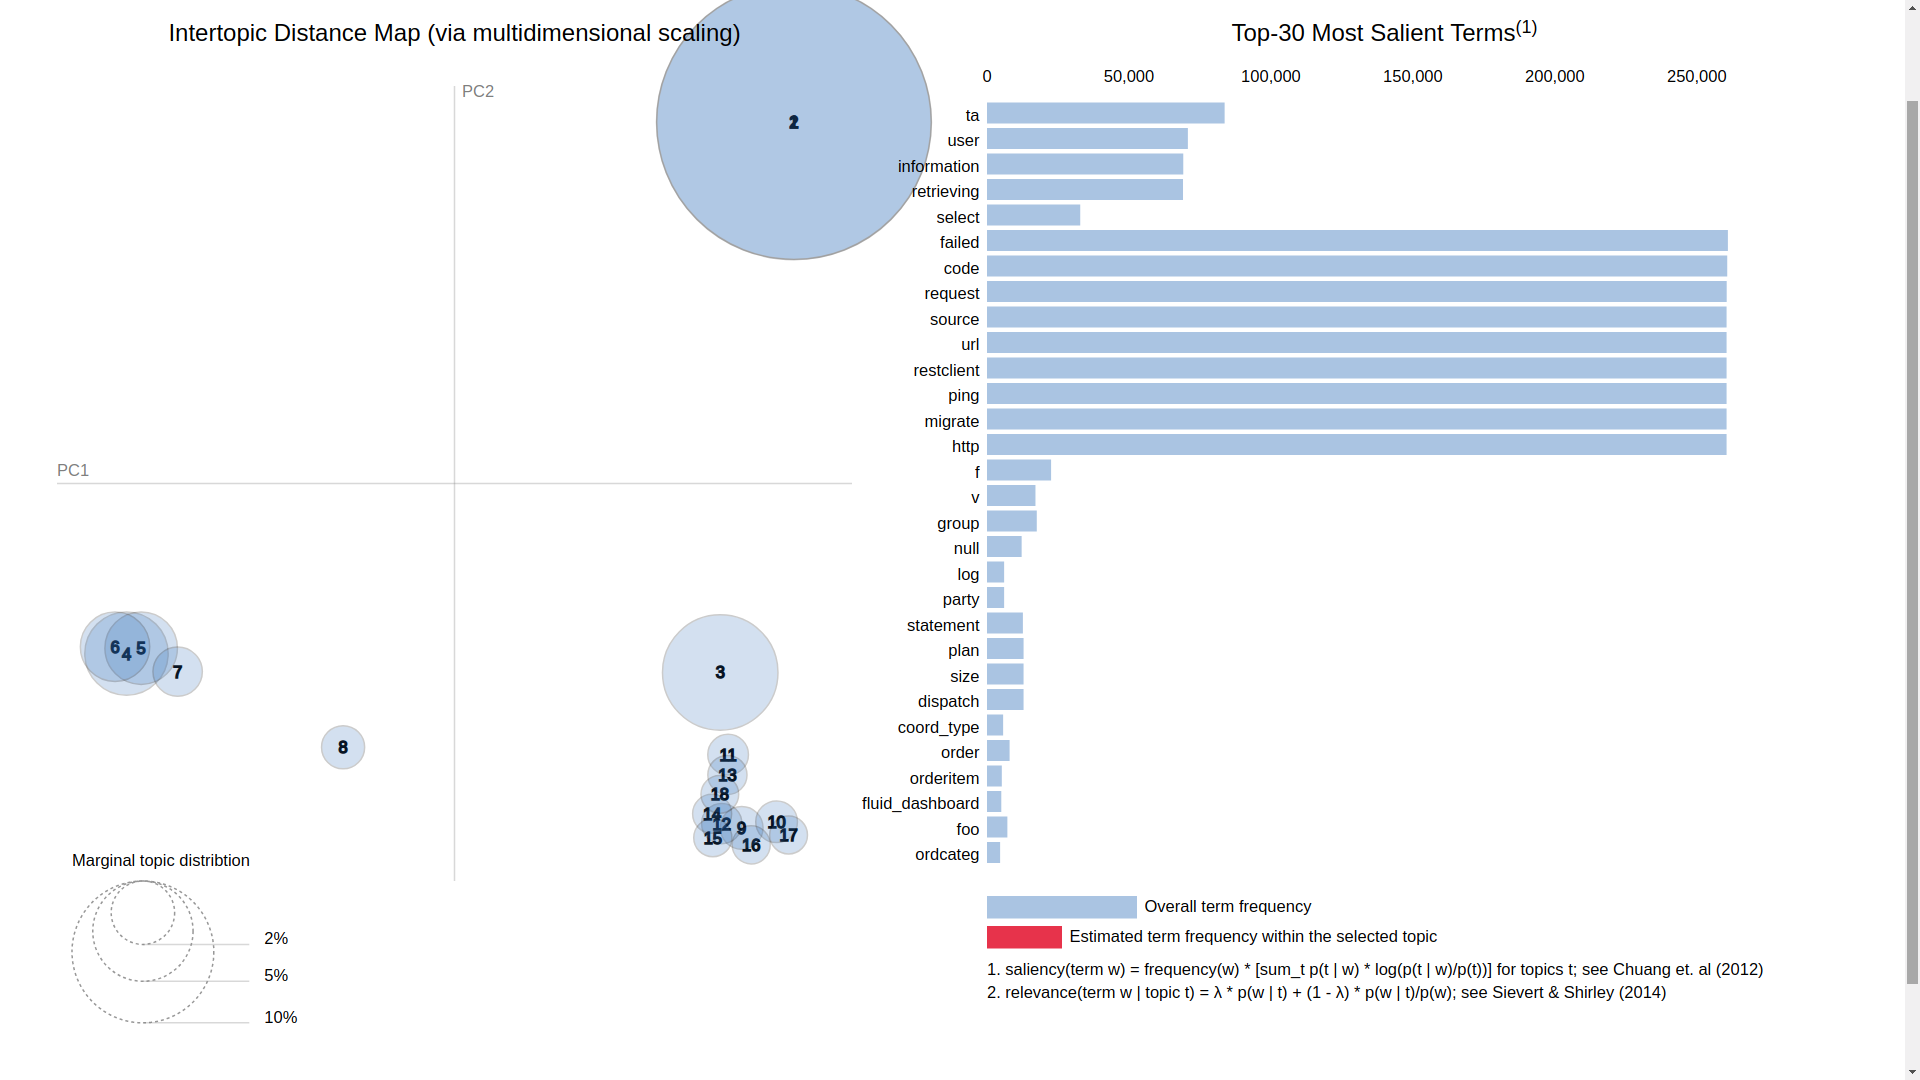
\includegraphics[width=15cm, height=8cm,trim=0 0 100px 0, clip=true]{figures/pyldavis/pyldavis_18.png}
    \caption{PyLdavis topic visualisation with 18 topics}
    \label{fig:pyldavis_18}
\end{figure}

 \begin{figure}[!h]
    \centering
    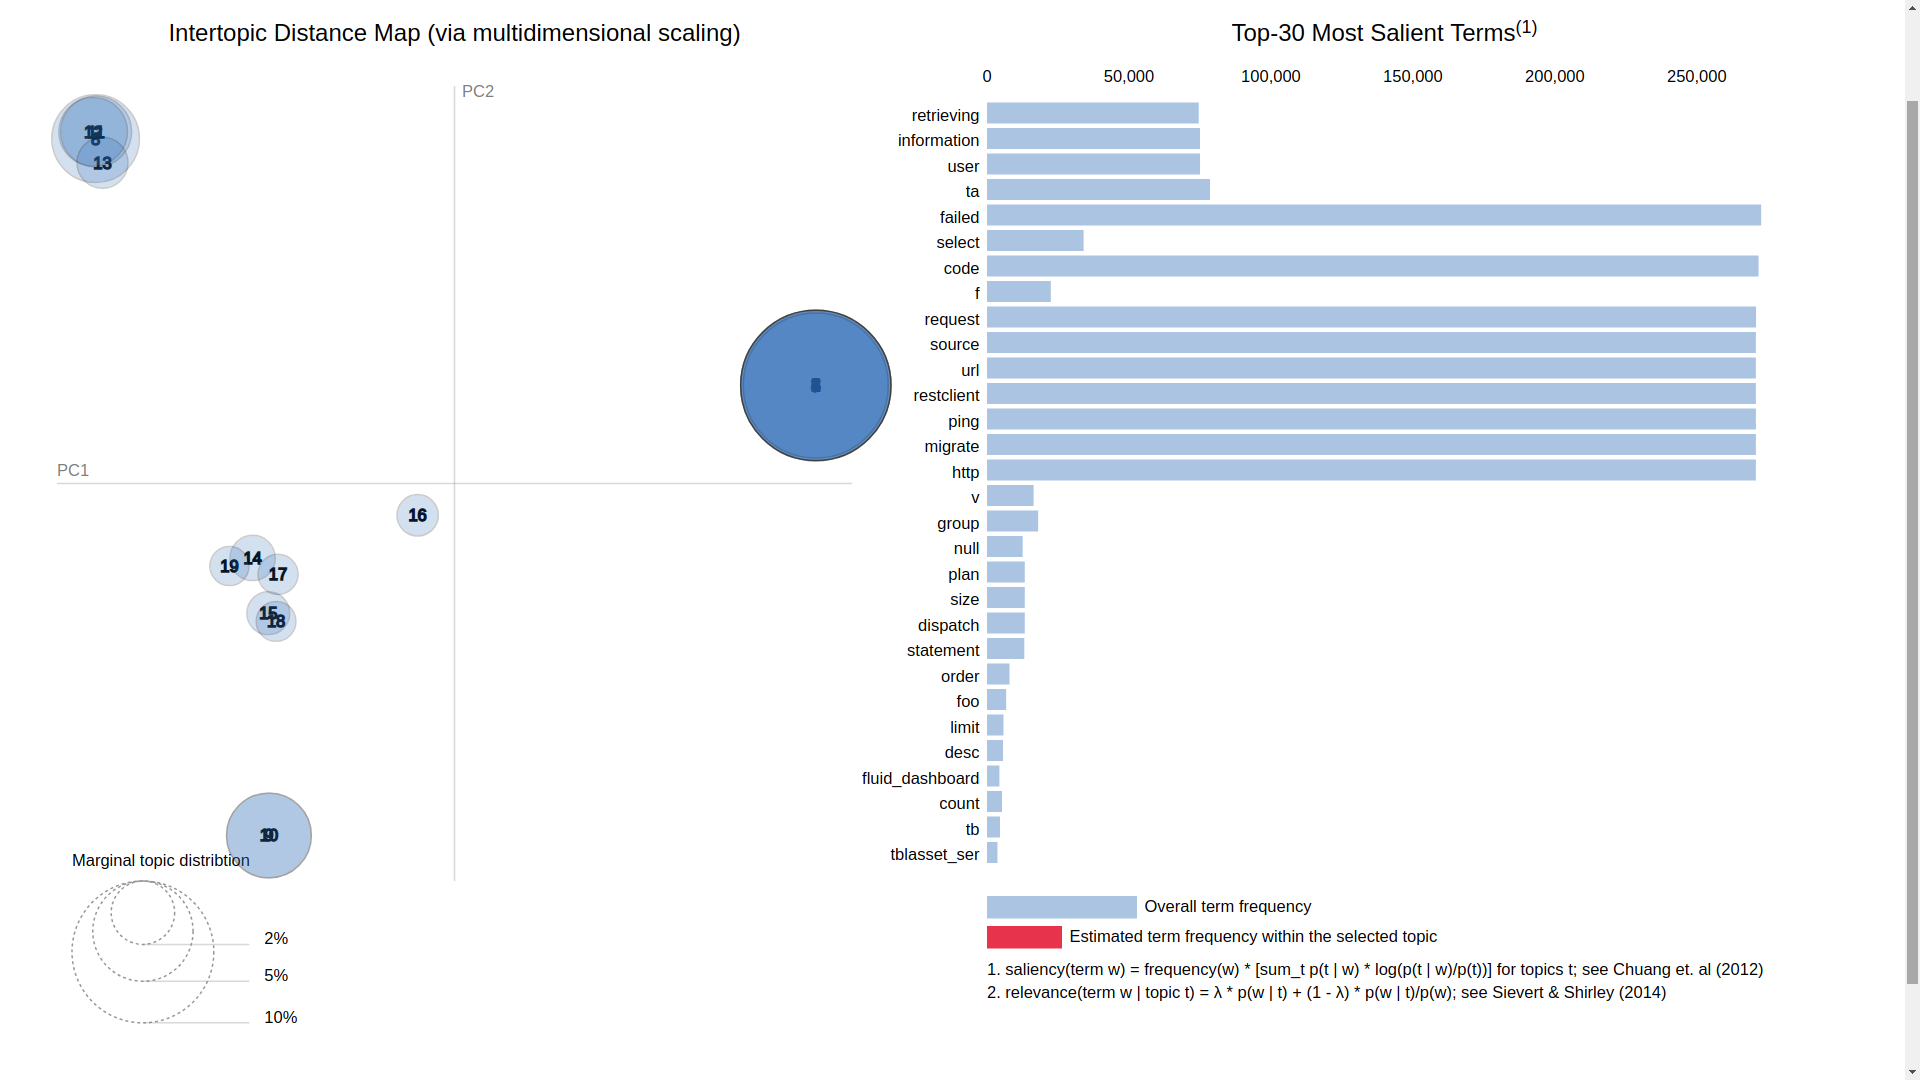
\includegraphics[width=15cm, height=8cm,trim=0 0 100px 0, clip=true]{figures/pyldavis/pyldavis_19.png}
    \caption{PyLdavis topic visualisation with 19 topics}
    \label{fig:pyldavis_19}
\end{figure}

 \begin{figure}[!h]
    \centering
    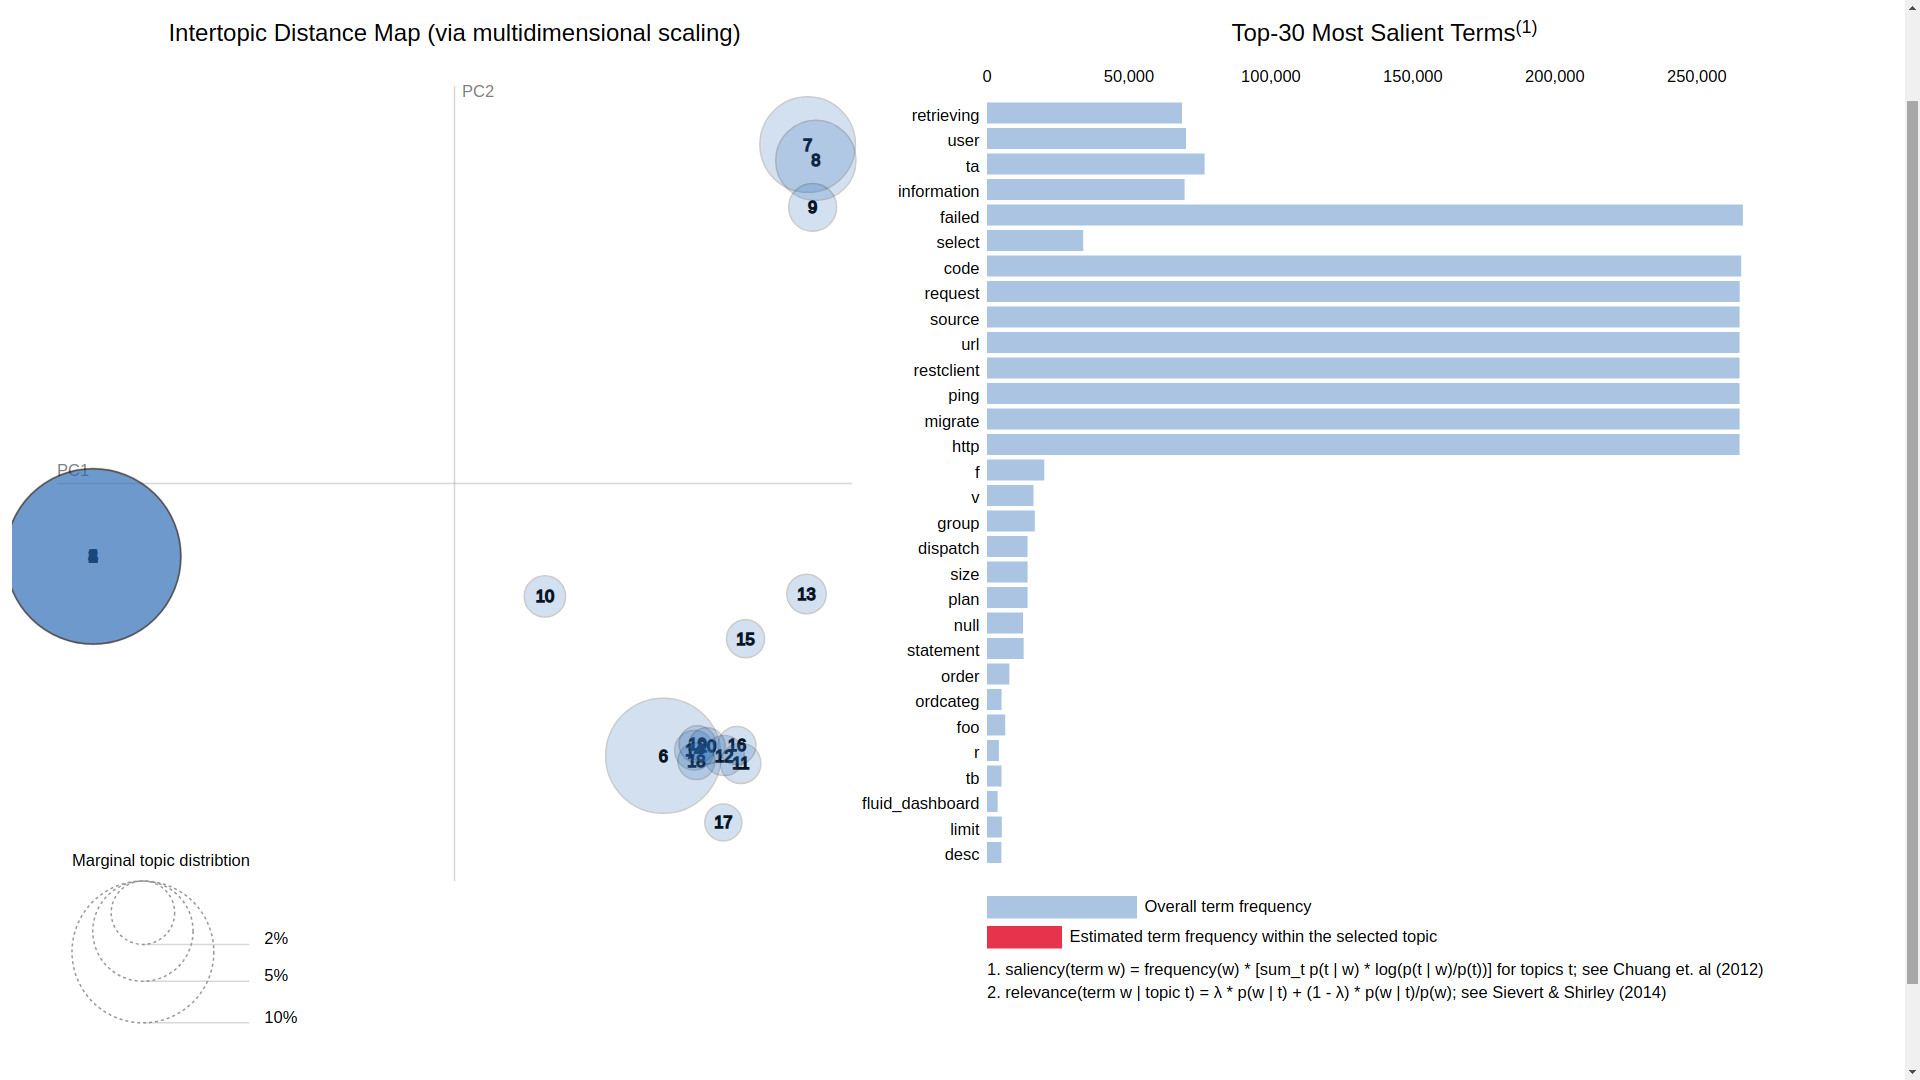
\includegraphics[width=15cm, height=8cm,trim=0 0 100px 0, clip=true]{figures/pyldavis/pyldavis_20.png}
    \caption{PyLdavis topic visualisation with 20 topics}
    \label{fig:pyldavis_20}
\end{figure}

 \begin{figure}[!h]
    \centering
    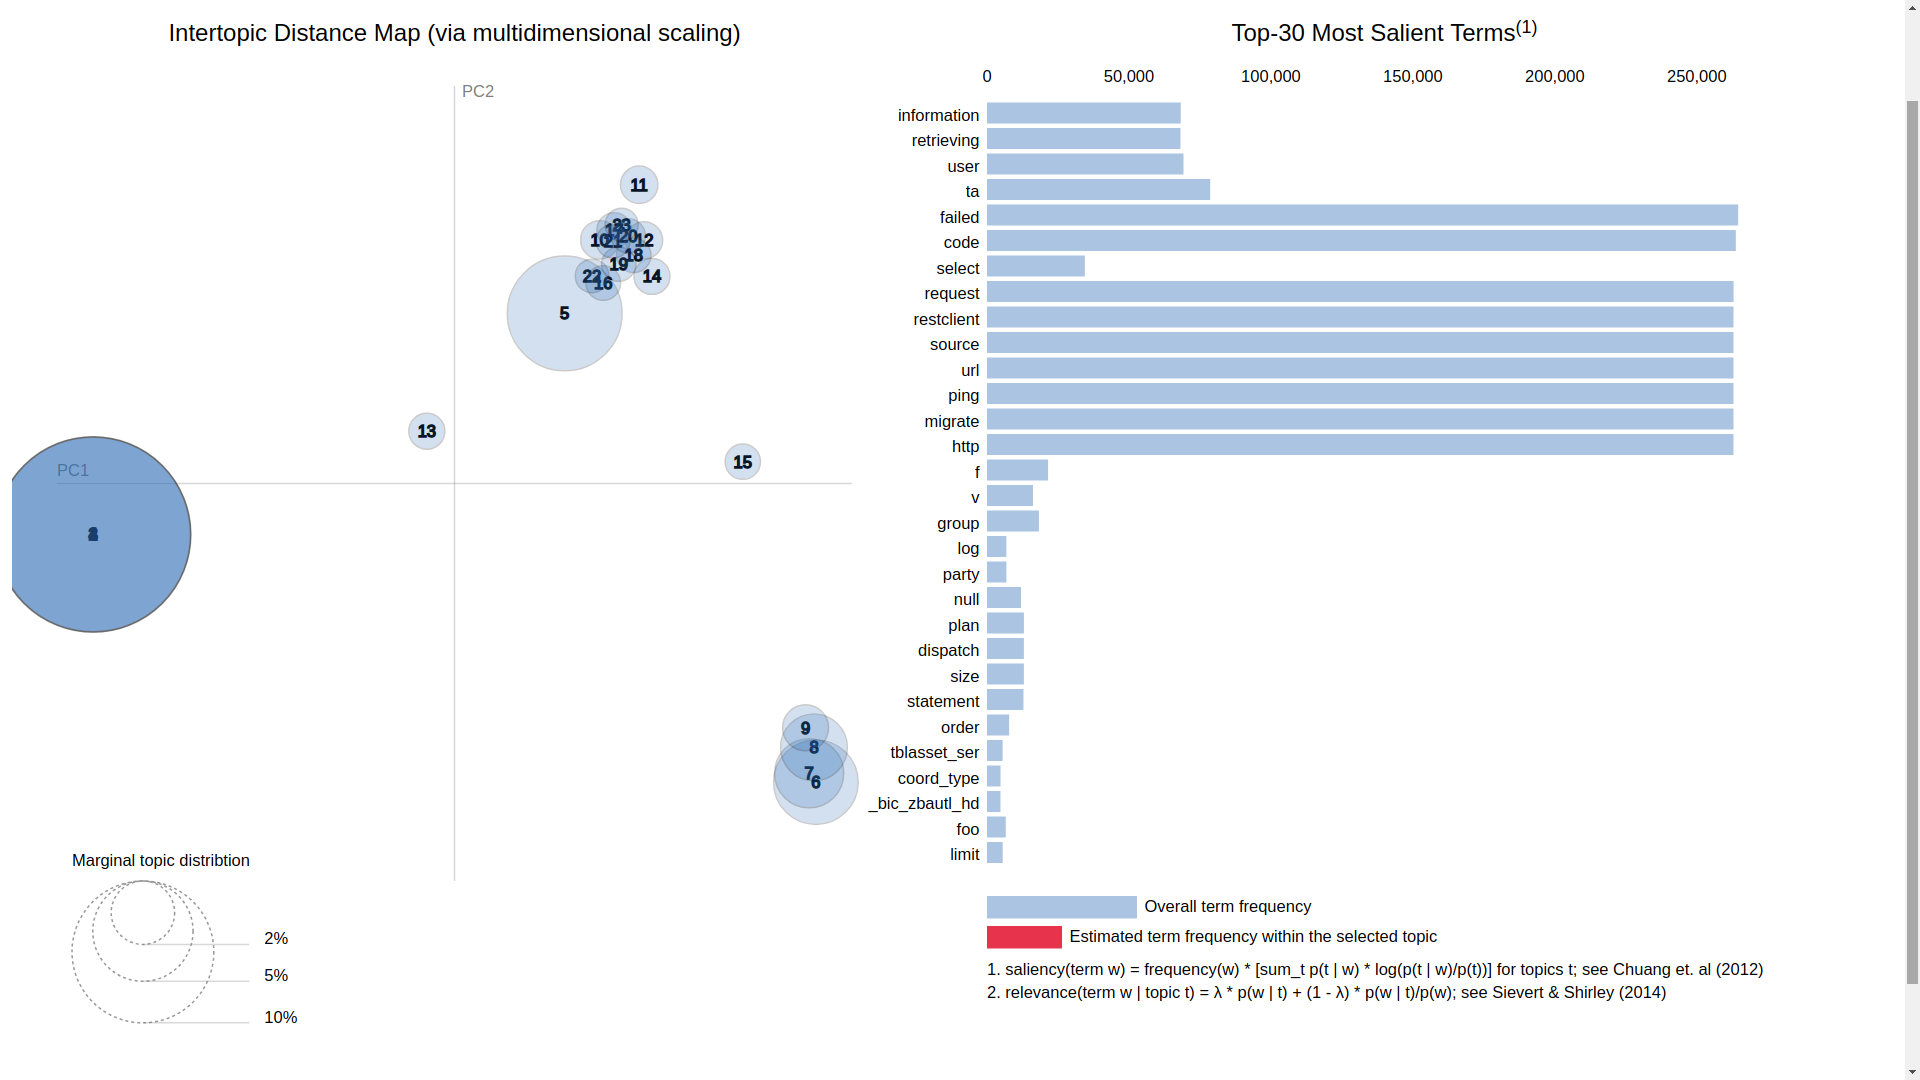
\includegraphics[width=15cm, height=8cm,trim=0 0 100px 0, clip=true]{figures/pyldavis/pyldavis_23.png}
    \caption{PyLdavis topic visualisation with 23 topics}
    \label{fig:pyldavis_23}
\end{figure}

 \begin{figure}[!h]
    \centering
    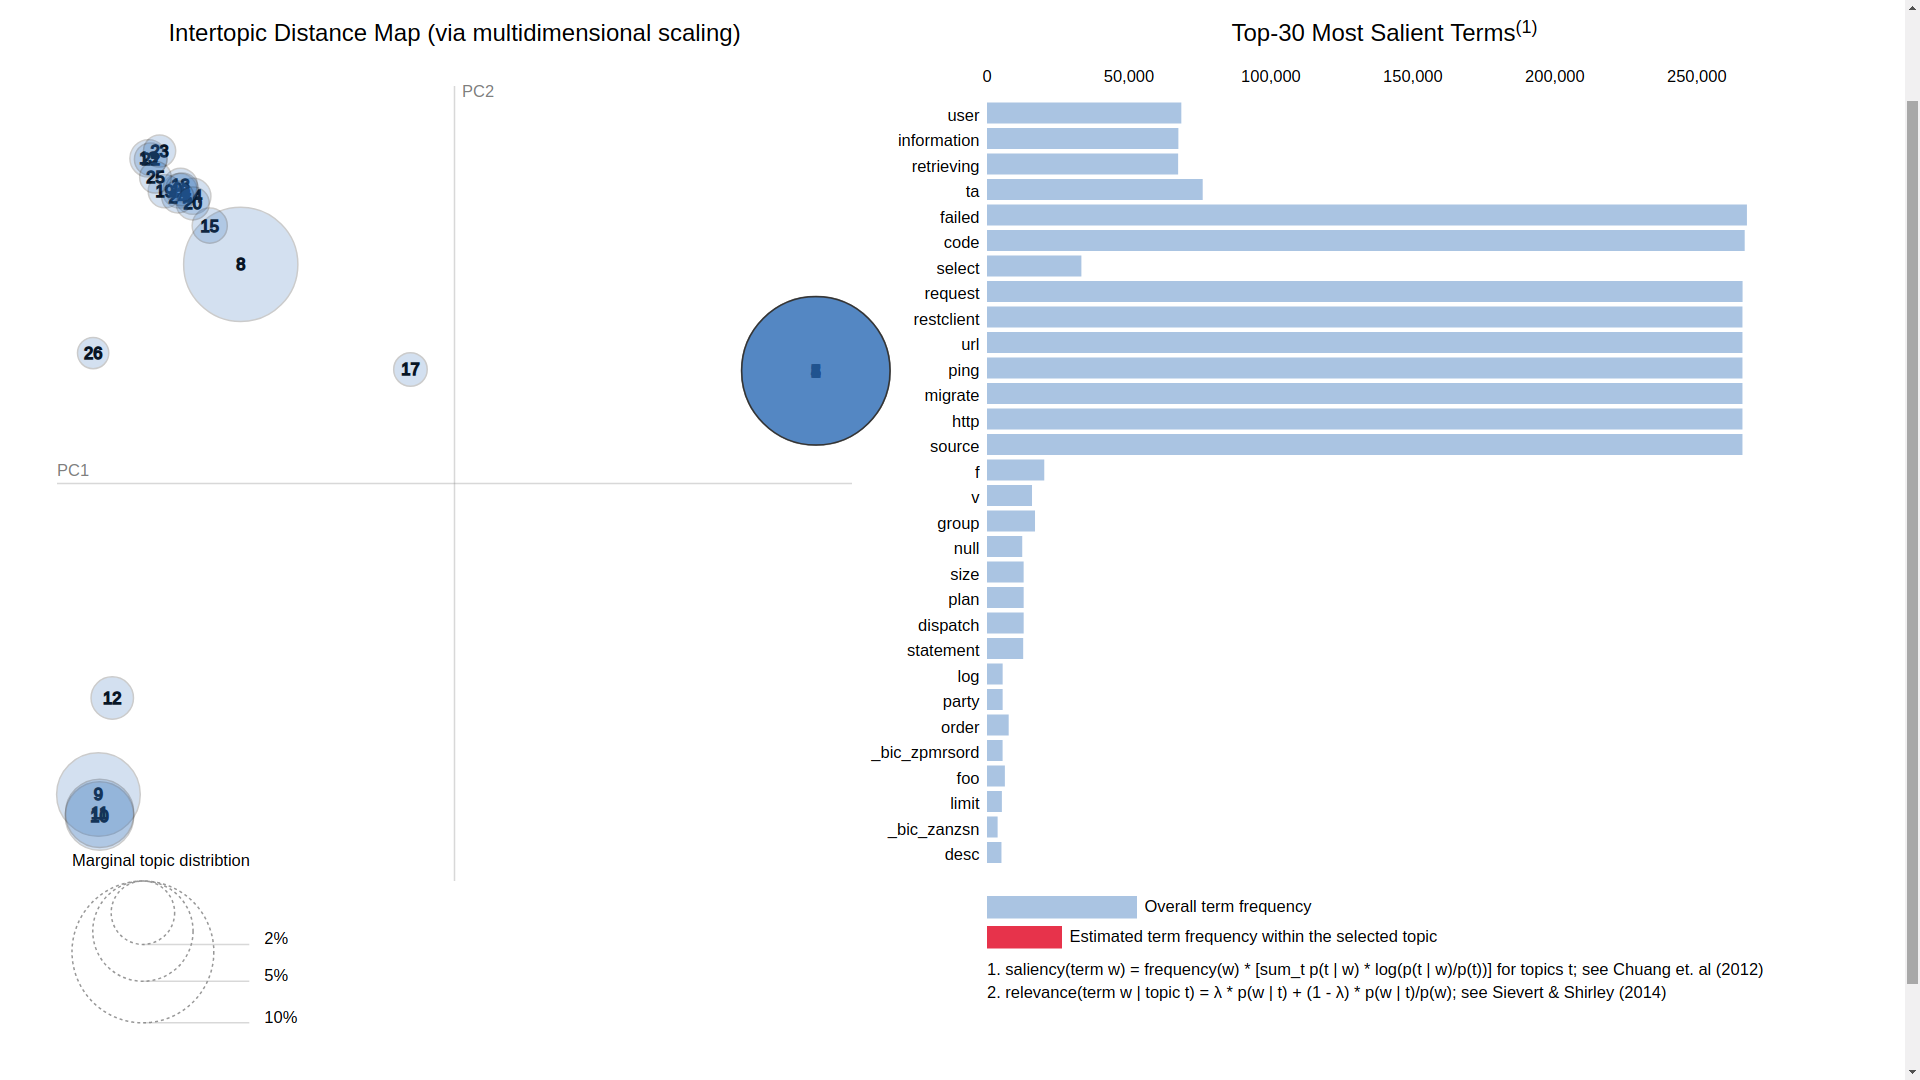
\includegraphics[width=15cm, height=8cm,trim=0 0 100px 0, clip=true]{figures/pyldavis/pyldavis_26.png}
    \caption{PyLdavis topic visualisation with 26 topics}
    \label{fig:pyldavis_26}
\end{figure}

 \begin{figure}[!h]
    \centering
    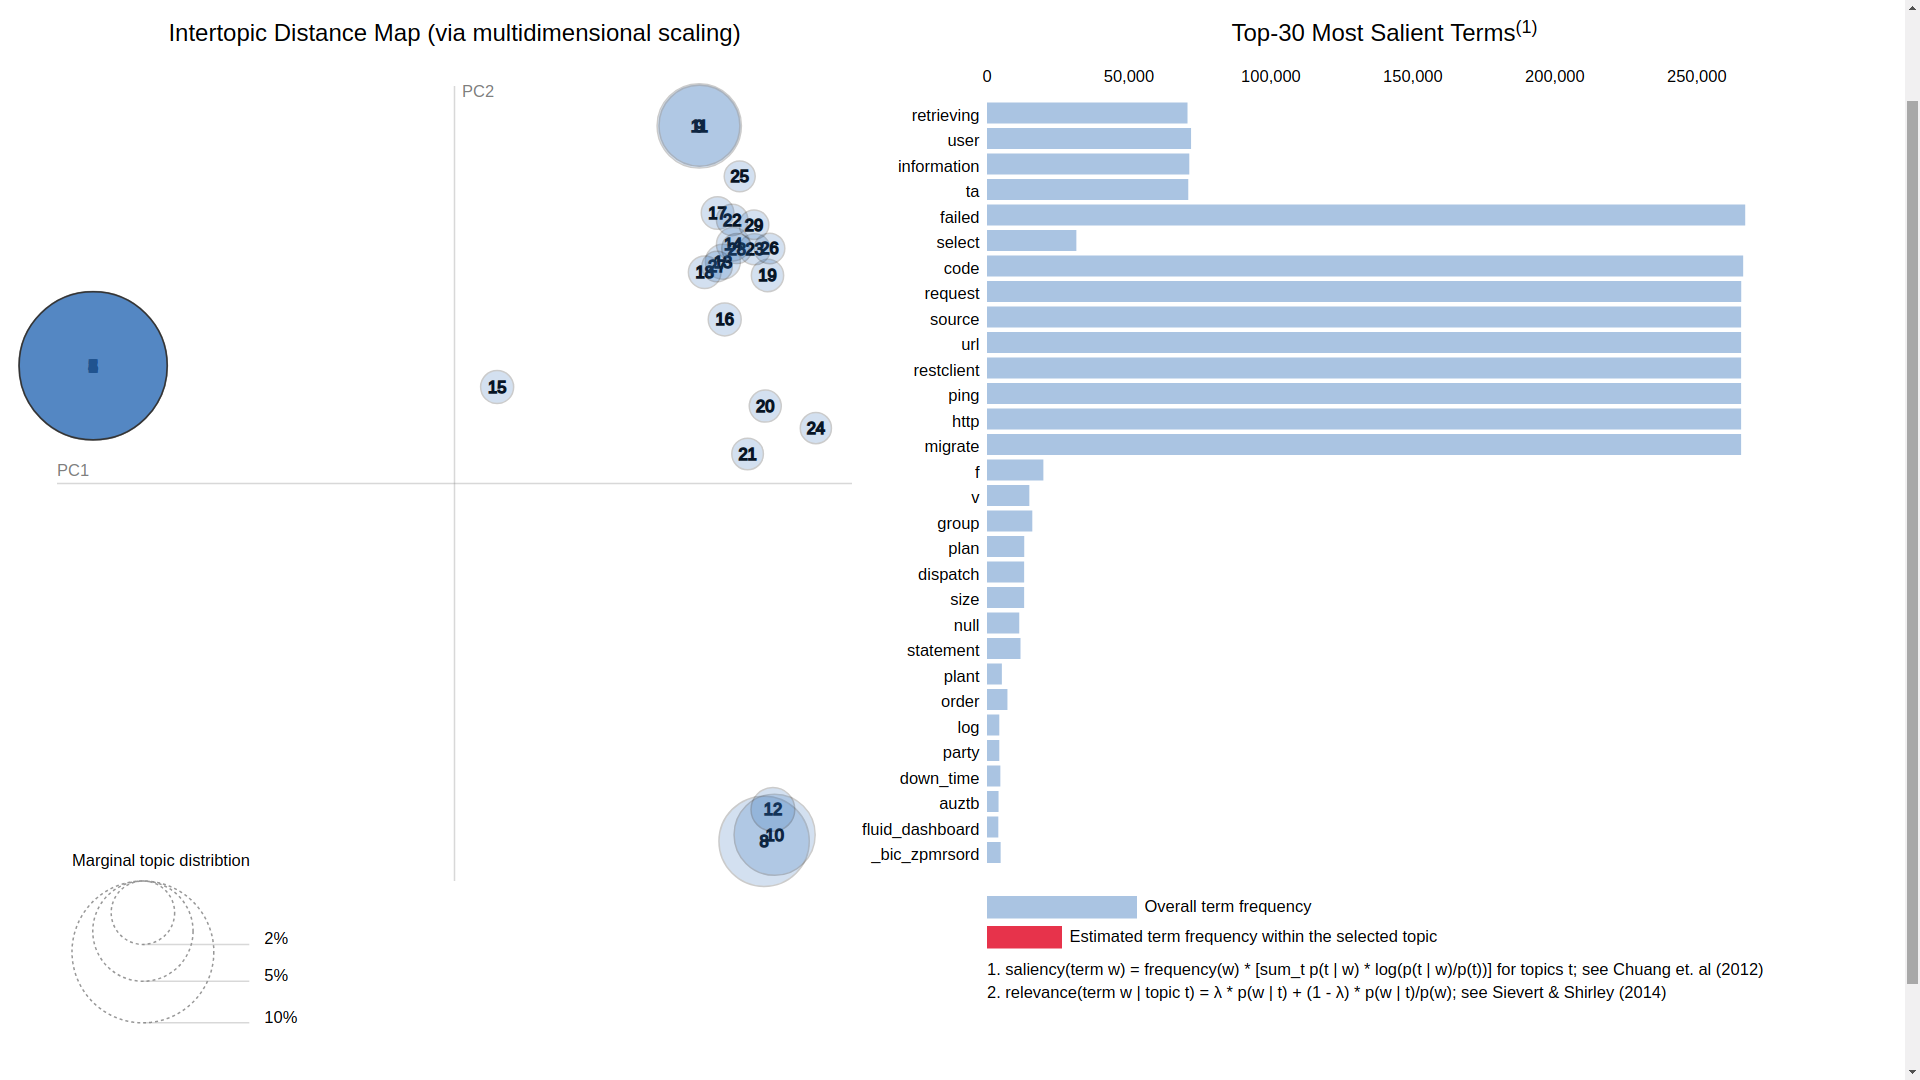
\includegraphics[width=15cm, height=8cm,trim=0 0 100px 0, clip=true]{figures/pyldavis/pyldavis_29.png}
    \caption{PyLdavis topic visualisation with 29 topics}
    \label{fig:pyldavis_29}
\end{figure}

 \begin{figure}[!h]
    \centering
    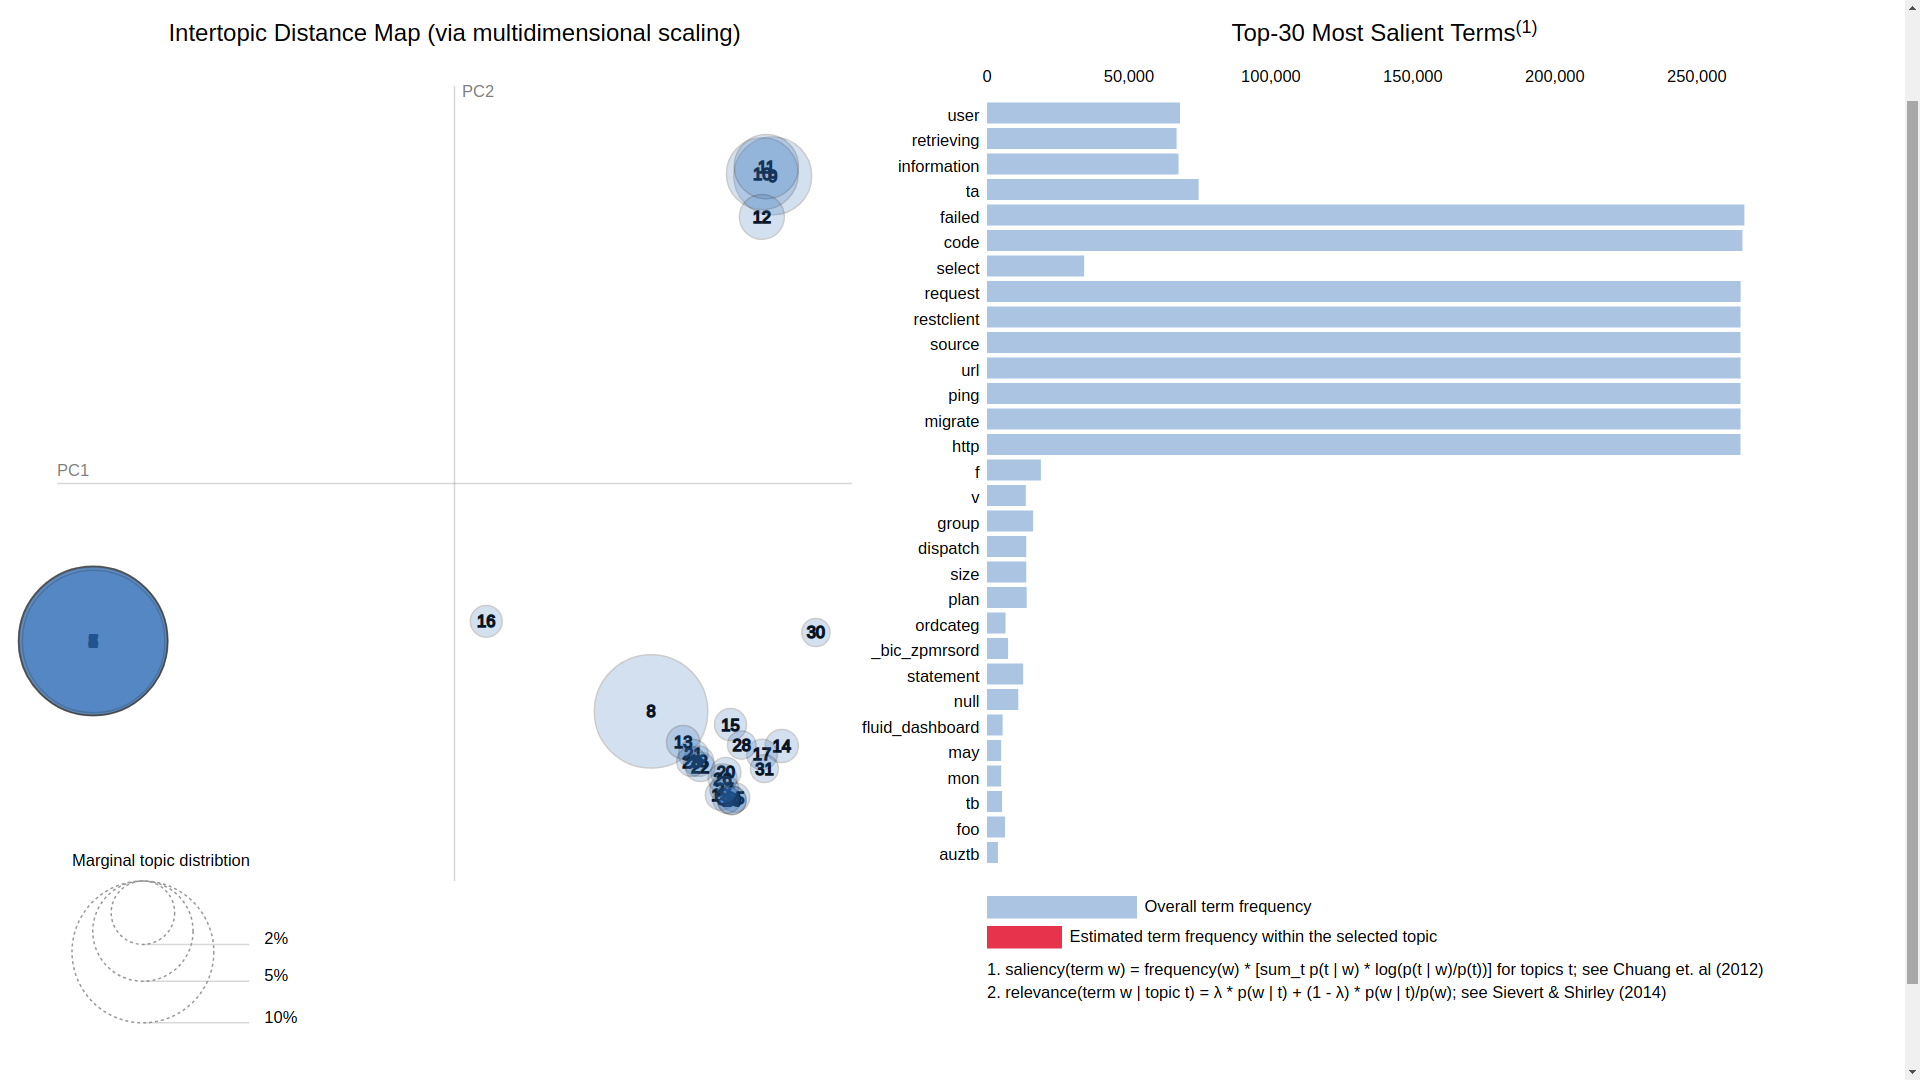
\includegraphics[width=15cm, height=8cm,trim=0 0 100px 0, clip=true]{figures/pyldavis/pyldavis_32.png}
    \caption{PyLdavis topic visualisation with 32 topics}
    \label{fig:pyldavis_32}
\end{figure}

 \begin{figure}[!h]
    \centering
    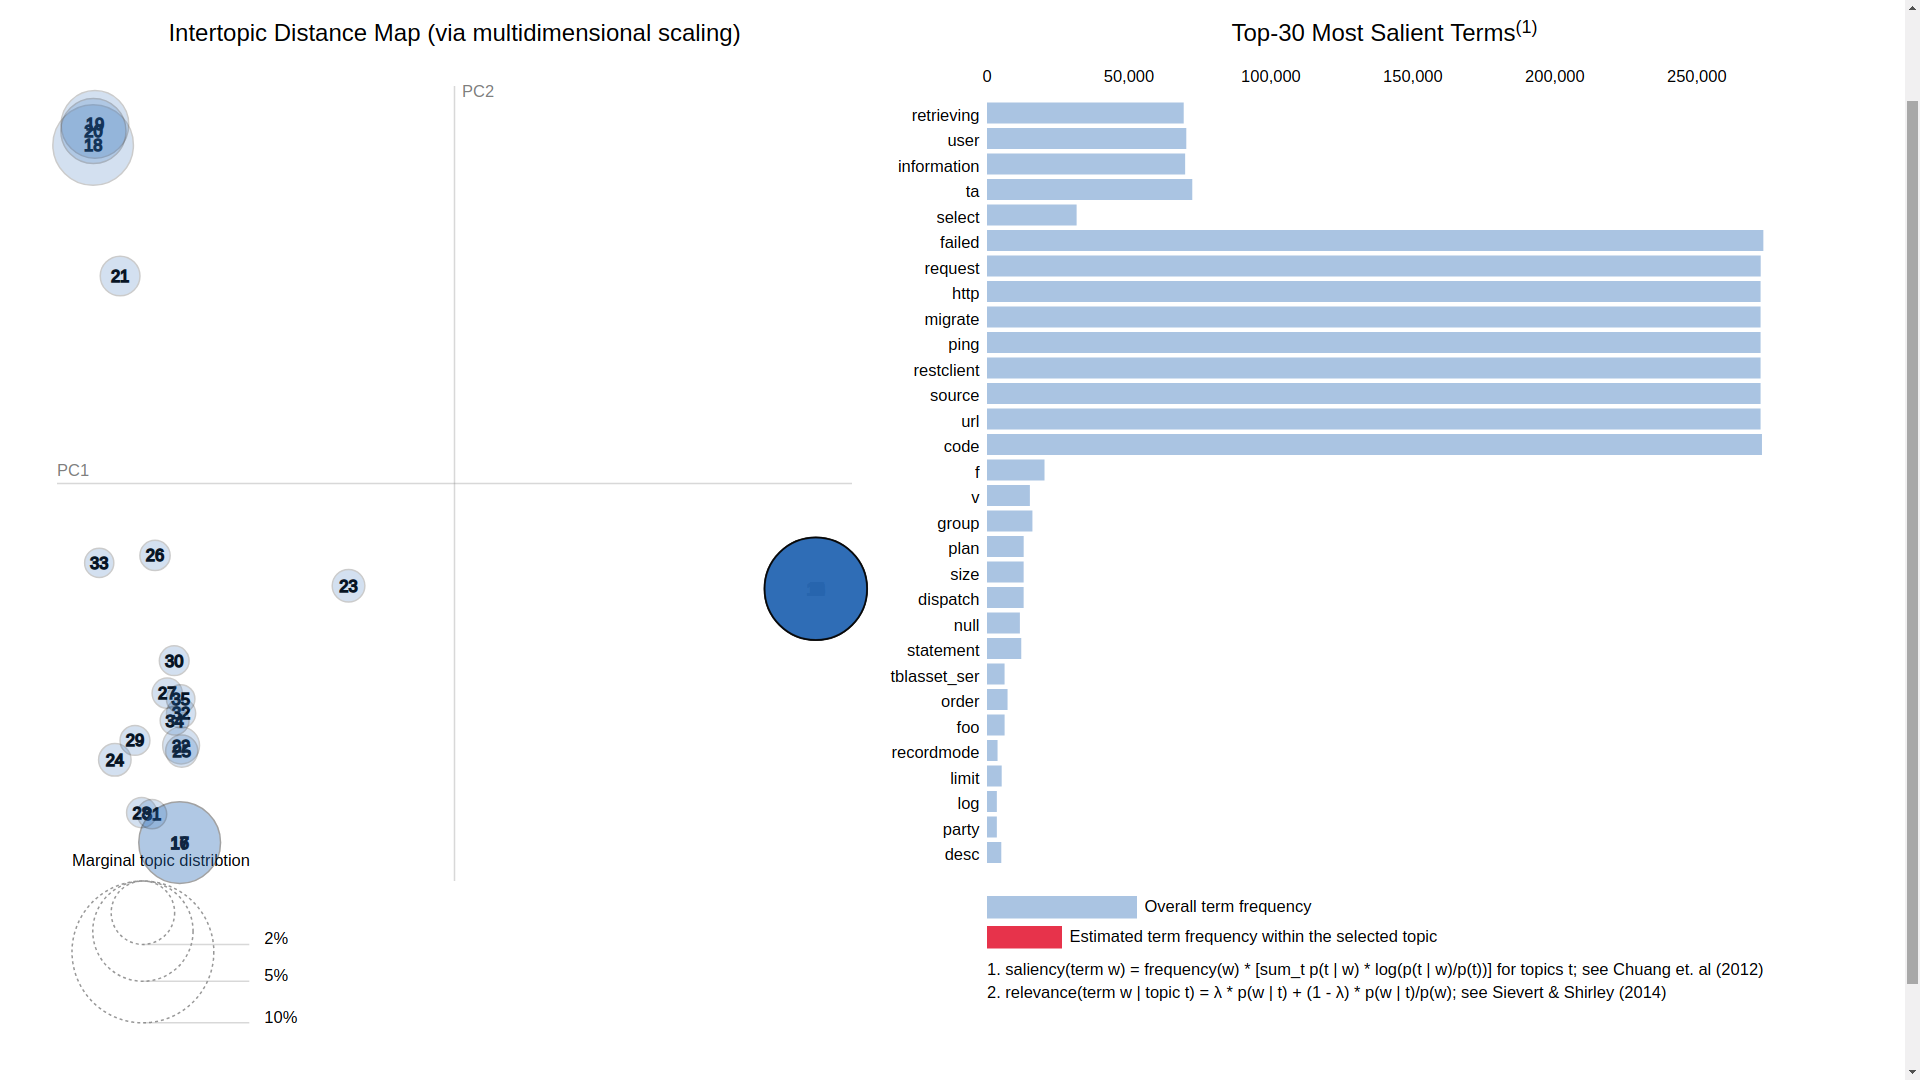
\includegraphics[width=15cm, height=8cm,trim=0 0 100px 0, clip=true]{figures/pyldavis/pyldavis_35.png}
    \caption{PyLdavis topic visualisation with 35 topics}
    \label{fig:pyldavis_35}
\end{figure}

 \begin{figure}[!h]
    \centering
    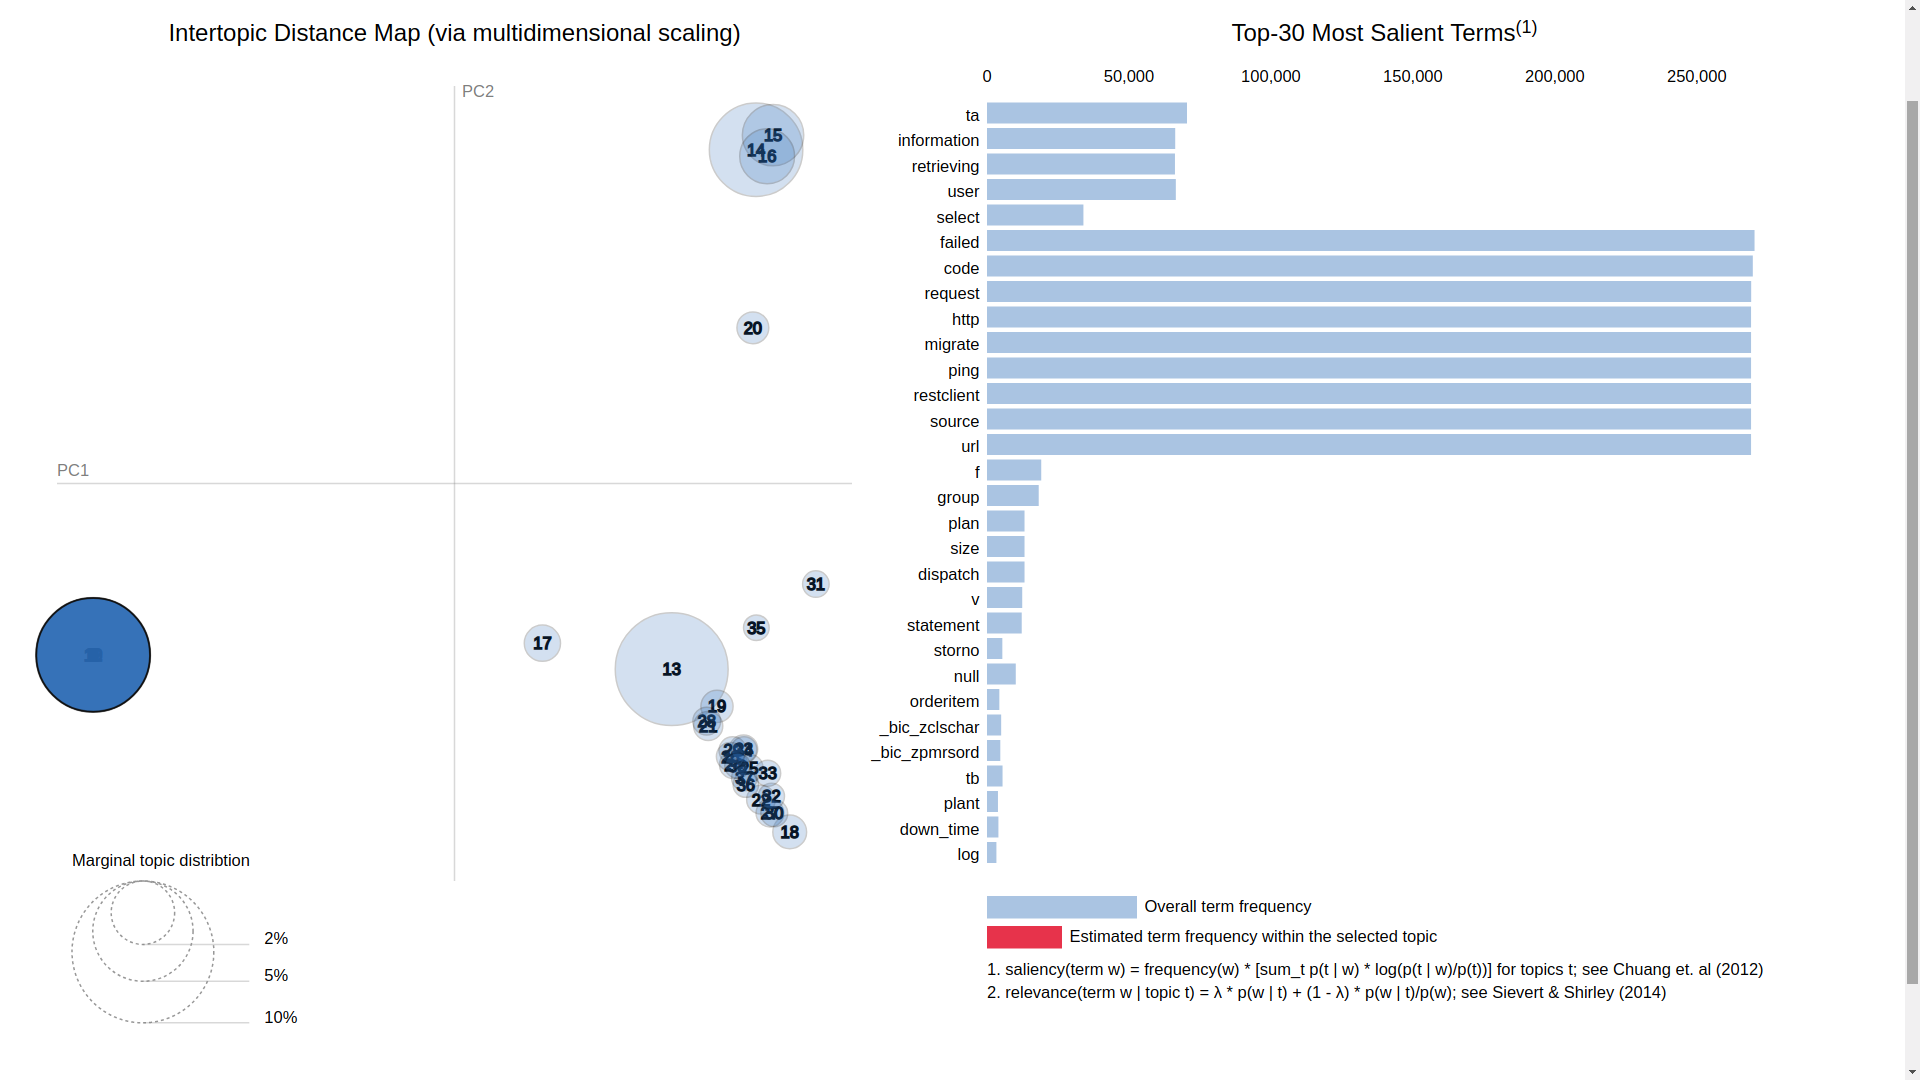
\includegraphics[width=15cm, height=8cm,trim=0 0 100px 0, clip=true]{figures/pyldavis/pyldavis_38.png}
    \caption{PyLdavis topic visualisation with 38 topics}
    \label{fig:pyldavis_38}
\end{figure}



\FloatBarrier
\section{Document distributions per amount of topics}\label{appendices:documentdistribution}

\subsection{Train test}
\begin{figure}[h]
    \centering
    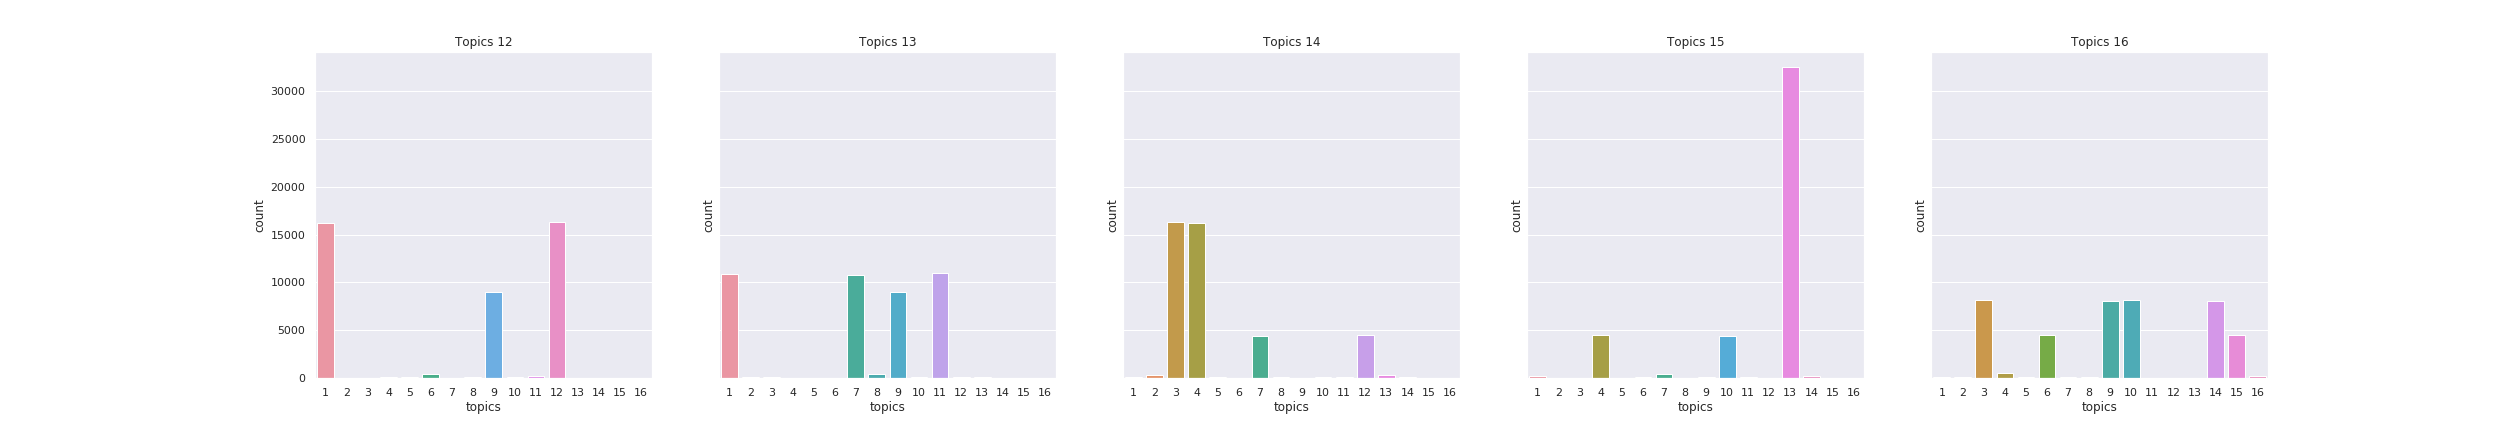
\includegraphics[width=15cm, height=8cm]{figures/doc_distr/doc_distribution_12-16.png}
    \caption{Document distribution with 12-16 topics}
    \label{fig:Doc_distr_12-16}
\end{figure}

\begin{figure}[h]
    \centering
    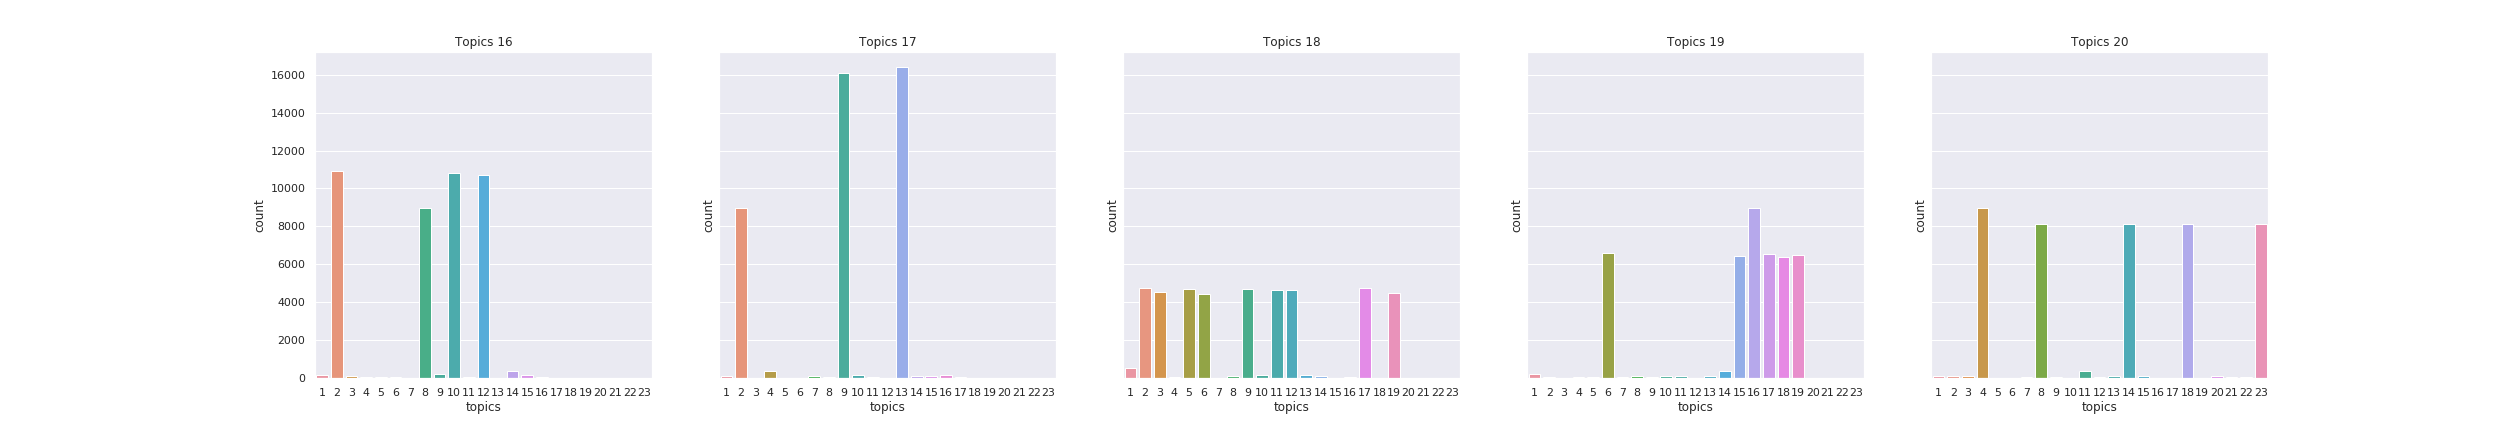
\includegraphics[width=15cm, height=8cm]{figures/doc_distr/doc_distribution_17-23.png}
    \caption{Document distribution with 17-23 topics}
    \label{fig:Doc_distr_17-21}
\end{figure}

\begin{figure}[h]
    \centering
    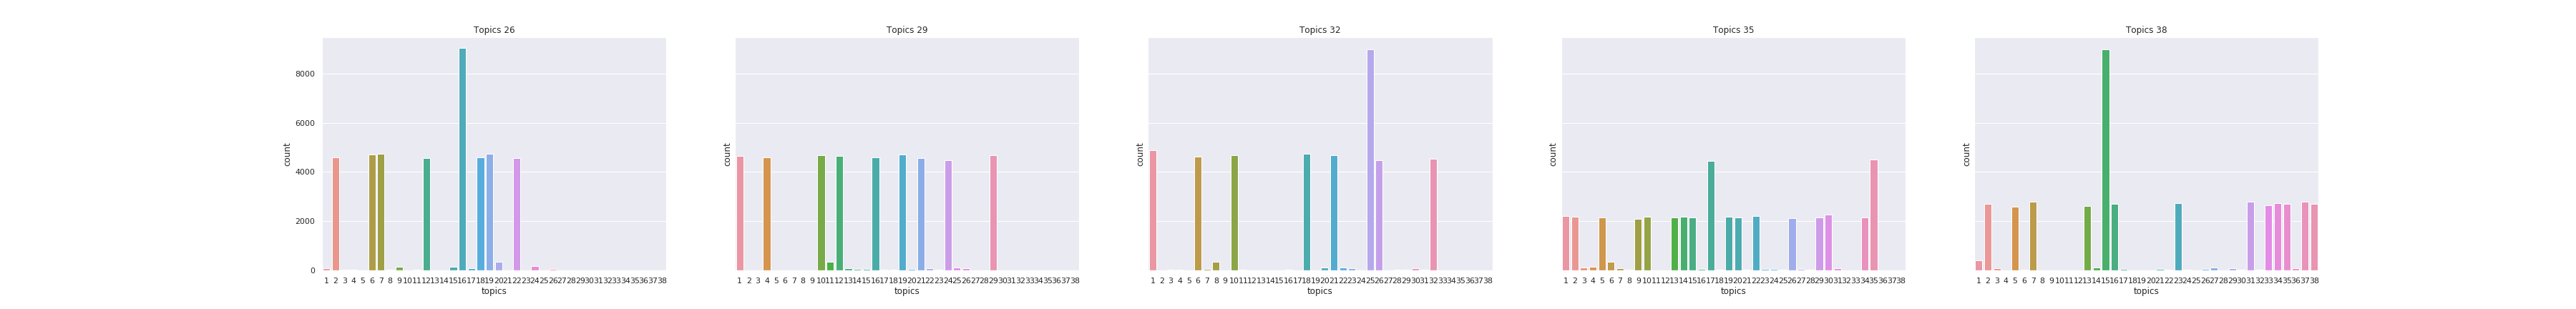
\includegraphics[width=15cm, height=8cm]{figures/doc_distr/doc_distribution_26-38.png}
    \caption{Document distribution with 26-38 topics}
    \label{fig:Doc_distr_26-38}
\end{figure}

\FloatBarrier

\subsection{Held out}
\begin{figure}[h]
    \centering
    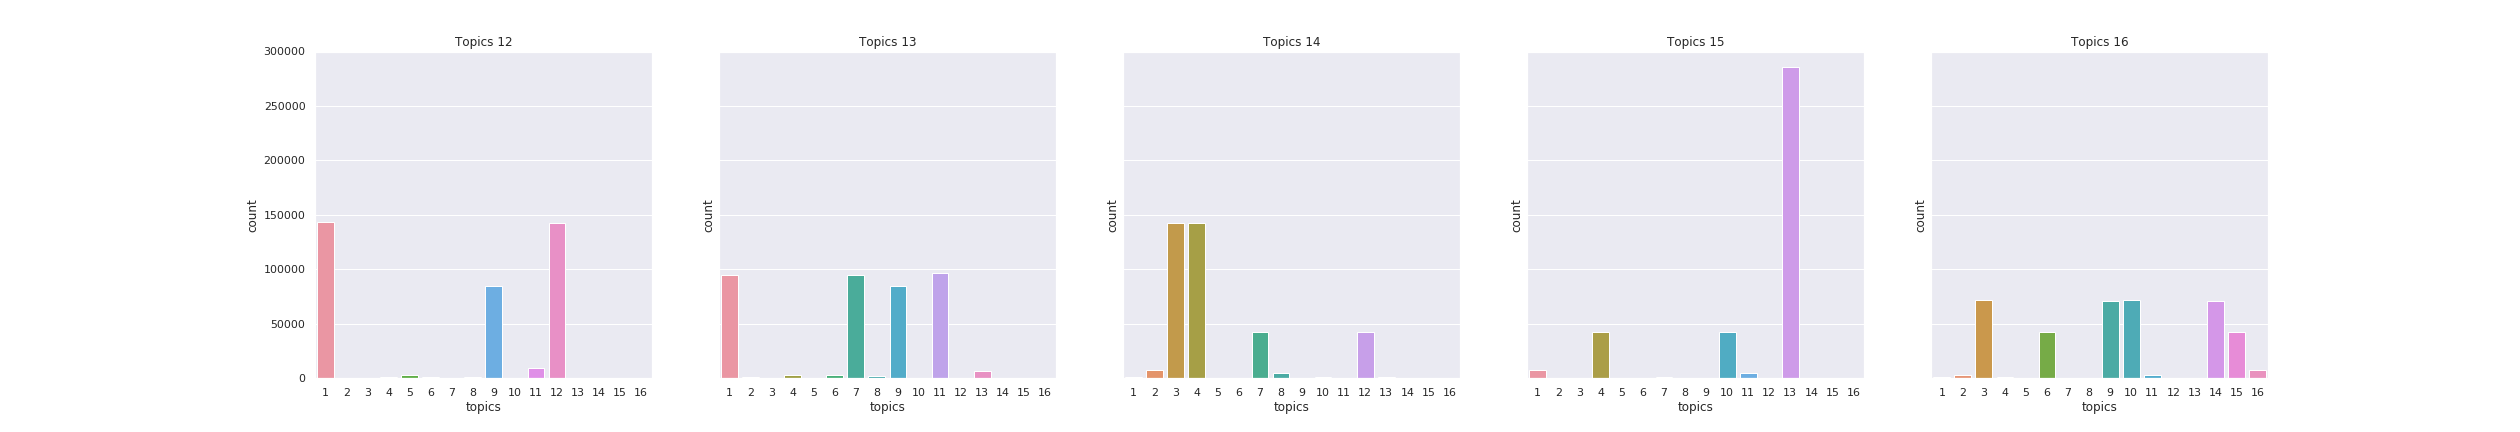
\includegraphics[width=15cm, height=8cm]{figures/doc_distr/doc_distribution_12-16_corpus.png}
    \caption{Document distribution with 12-16 topics}
    \label{fig:Doc_distr_12-16}
\end{figure}

\begin{figure}[h]
    \centering
    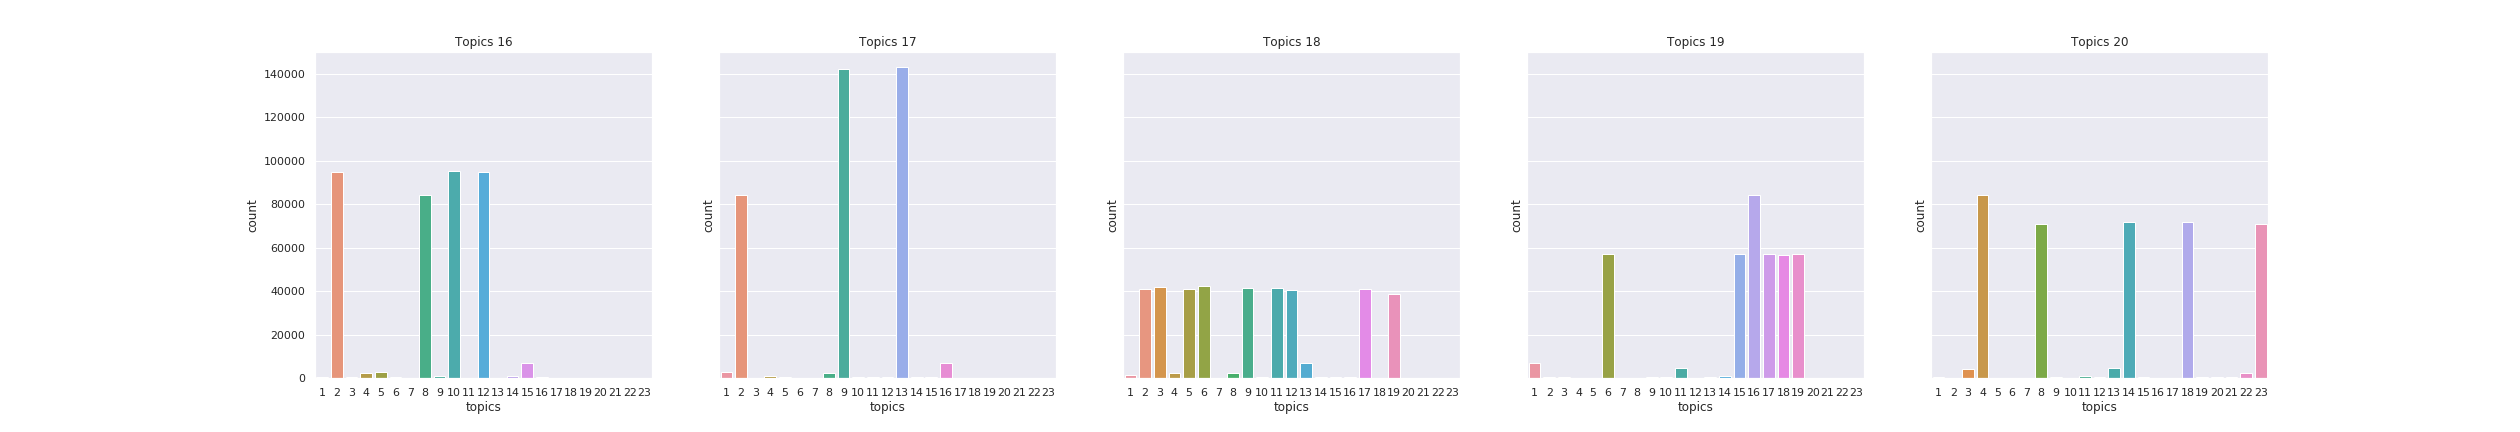
\includegraphics[width=15cm, height=8cm]{figures/doc_distr/doc_distribution_17-23_corpus.png}
    \caption{Document distribution with 17-23 topics}
    \label{fig:Doc_distr_17-21}
\end{figure}

\begin{figure}[h]
    \centering
    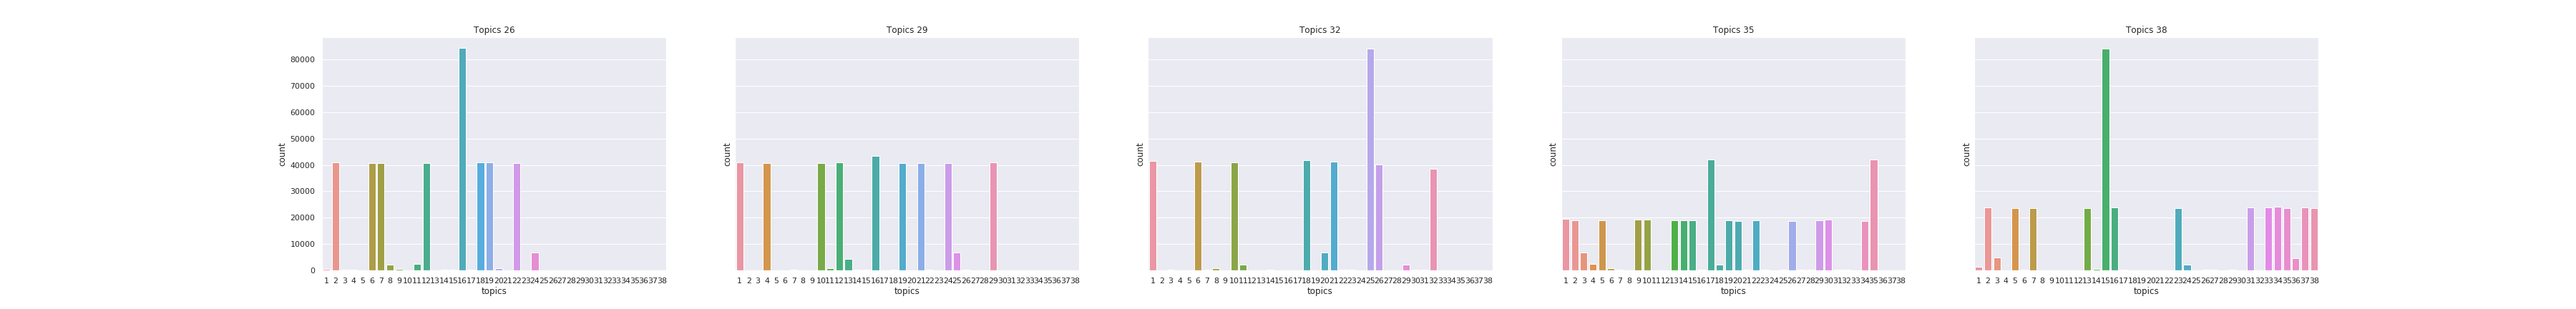
\includegraphics[width=15cm, height=8cm]{figures/doc_distr/doc_distribution_26-38_corpus.png}
    \caption{Document distribution with 26-38 topics}
    \label{fig:Doc_distr_26-38}
\end{figure}



\FloatBarrier
\section{Model generated topics}\label{appendices:modelgeneratedtopics}

\begin{table}[!htb]
\centering
\begin{tabular}{|l|l|l|l|l|l|}
 \hline
 Topic & Terms & & & & \\
 \hline
 0 & failed & code & request & source & ping\\ 
 \hline 
 1 & ta & select & f & group & plan\\ 
 \hline 
 2 & user & information & retrieving & text & log\\ 
 \hline 
\end{tabular}
\caption{Topic 1..3 with top 5 terms}
\label{tab:3topicsmodel}
\end{table}
 
\begin{table}[!htb]
\centering
\begin{tabular}{|l|l|l|l|l|l|}
 \hline
 Topic & Terms & & & & \\
 \hline
 0 & fluid\_dashboard & text & tblasset\_ser & recordmode & log\\ 
 \hline 
 1 & ta & select & f & group & plan\\ 
 \hline 
 2 & user & information & retrieving & cancel & token\\ 
 \hline 
 3 & failed & code & request & source & restclient\\ 
 \hline 
\end{tabular}
\caption{Topic 1..4 with top 5 terms}
\label{tab:4topicsmodel}
\end{table}
 
 
\begin{table}[!htb]
\centering
\begin{tabular}{|l|l|l|l|l|l|}
 \hline
 Topic & Terms & & & & \\
 \hline
 0 & failed & code & request & source & url\\ 
 \hline 
 1 & fluid\_dashboard & text & tblasset\_ser & tbljob\_sow & coord\_type\\ 
 \hline 
 2 & user & information & retrieving & controller & could\\ 
 \hline 
 3 & count & plant & redo & customer & record\\ 
 \hline 
 4 & ta & select & f & group & plan\\ 
 \hline 
 5 & v & order & r & null & tb\\ 
 \hline 
\end{tabular}
\caption{Topic 1..6 with top 5 terms}
\label{tab:6topicsmodel}
\end{table}
 
\begin{table}[!htb]
\centering
\begin{tabular}{|l|l|l|l|l|l|}
 \hline
 Topic & Terms & & & & \\
 \hline
 0 & ta & select & size & dispatch & plan\\ 
 \hline 
 1 & notificatn & coord\_type & rowcnt & tblasset\_ser & \_bic\_zvorgang\\ 
 \hline 
 2 & user & information & retrieving & terminated & slice\_id\\ 
 \hline 
 3 & f & v & group & limit & desc\\ 
 \hline 
 4 & fluid\_dashboard & text & tblasset\_ser & tbljob\_sow & orderitem\\ 
 \hline 
 5 & v & r & order & tb & null\\ 
 \hline 
 6 & failed & code & request & url & source\\ 
 \hline 
\end{tabular}
\caption{Topic 1..7 with top 5 terms}
\label{tab:7topicsmodel}
\end{table}
 
\begin{table}[!htb]
\centering
\begin{tabular}{|l|l|l|l|l|l|}
 \hline
 Topic & Terms & & & & \\
 \hline
 0 & request & ping & source & restclient & url\\ 
 \hline 
 1 & log & party & \_bic\_zanzsn & orderitem & \_bic\_zvorgang\\ 
 \hline 
 2 & request & ping & migrate & source & http\\ 
 \hline 
 3 & coord\_type & ordcateg & cancel & token & \_bic\_zpmrsord\\ 
 \hline 
 4 & user & information & retrieving & may & mon\\ 
 \hline 
 5 & ta & select & f & group & plan\\ 
 \hline 
 6 & failed & plant & group & code & controller\\ 
 \hline 
 7 & fluid\_dashboard & text & tblasset\_ser & tbljob\_sow & rowcnt\\ 
 \hline 
\end{tabular}
\caption{Topic 1..8 with top 5 terms}
\label{tab:8topicsmodel}
\end{table}
 
\begin{table}[!htb]
\centering
\begin{tabular}{|l|l|l|l|l|l|}
 \hline
 Topic & Terms & & & & \\
 \hline
 0 & ta & f & group & limit & desc\\ 
 \hline 
 1 & fluid\_dashboard & text & tblasset\_ser & tbljob\_sow & may\\ 
 \hline 
 2 & log & party & coord\_type & storno & employee\\ 
 \hline 
 3 & ta & select & size & dispatch & plan\\ 
 \hline 
 4 & failed & code & request & source & url\\ 
 \hline 
 5 & ordcateg & unit\_day & auztb & ops & hawqstatus\\ 
 \hline 
 6 & user & information & retrieving & terminated & stage\\ 
 \hline 
 7 & cancel & rowcnt & redo & token & record\\ 
 \hline 
 8 & v & r & select & null & order\\ 
 \hline 
\end{tabular}
\caption{Topic 1..9 with top 5 terms}
\label{tab:9topicsmodel}
\end{table}
 
 
\begin{table}[!htb]
\centering
\begin{tabular}{|l|l|l|l|l|l|}
 \hline
 Topic & Terms & & & & \\
 \hline
 0 & request & ping & source & restclient & url\\ 
 \hline 
 1 & failed & group & controller & code & could\\ 
 \hline 
 2 & ta & select & plan & dispatch & size\\ 
 \hline 
 3 & \_bic\_zanzsn & orderitem & \_bic\_zvorgang & \_bic\_zpmrsord & set\\ 
 \hline 
 4 & coord\_type & storno & unit\_day & division & employee\\ 
 \hline 
 5 & ta & f & group & v & select\\ 
 \hline 
 6 & request & source & url & restclient & code\\ 
 \hline 
 7 & user & information & retrieving & tblasset\_ser & tbljob\_sow\\ 
 \hline 
 8 & ta & v & select & null & r\\ 
 \hline 
 9 & plant & redo & customer & record & length\\ 
 \hline 
 10 & fluid\_dashboard & text & tblasset\_ser & log & party\\ 
 \hline 
\end{tabular}
\caption{Topic 1..11 with top 5 terms}
\label{tab:11topicsmodel}
\end{table}
 
\begin{table}[!htb]
\centering
\begin{tabular}{|l|l|l|l|l|l|}
 \hline
 Topic & Terms & & & & \\
 \hline
 0 & request & ping & migrate & source & http\\ 
 \hline 
 1 & plant & redo & customer & record & length\\ 
 \hline 
 2 & ordcateg & unit\_day & notif\_orgn & down\_time & auztv\\ 
 \hline 
 3 & failed & controller & group & code & could\\ 
 \hline 
 4 & ta & f & order & v & null\\ 
 \hline 
 5 & fluid\_dashboard & text & log & party & tblasset\_ser\\ 
 \hline 
 6 & ta & material & recordmode & notificatn & createdon\\ 
 \hline 
 7 & tblasset\_ser & cancel & tbljob\_sow & orderitem & token\\ 
 \hline 
 8 & information & user & retrieving & \_bic\_zpmrsord & \_bic\_zobjvw\\ 
 \hline 
 9 & \_bic\_zanzsn & coord\_type & may & mon & \_bic\_zvorgang\\ 
 \hline 
 10 & ta & select & group & plan & dispatch\\ 
 \hline 
 11 & request & ping & source & restclient & url\\ 
 \hline 
\end{tabular}
\caption{Topic 1..12 with top 5 terms}
\label{tab:12topicsmodel}
\end{table}
 
\begin{table}[!htb]
\centering
\begin{tabular}{|l|l|l|l|l|l|}
 \hline
 Topic & Terms & & & & \\
 \hline
 0 & request & ping & url & source & restclient\\ 
 \hline 
 1 & failed & group & controller & code & could\\ 
 \hline 
 2 & cancel & token & postgres & auztb & user\\ 
 \hline 
 3 & ta & f & v & order & null\\ 
 \hline 
 4 & coord\_type & rowcnt & storno & unit\_day & division\\ 
 \hline 
 5 & ta & f & select & v & group\\ 
 \hline 
 6 & request & ping & url & source & restclient\\ 
 \hline 
 7 & fluid\_dashboard & text & tblasset\_ser & log & party\\ 
 \hline 
 8 & information & retrieving & user & \_bic\_zpmrsord & \_bic\_zobjvw\\ 
 \hline 
 9 & \_bic\_zanzsn & \_bic\_zvorgang & \_bic\_zqmdat & \_bic\_zbautl\_hd & set\\ 
 \hline 
 10 & request & code & failed & source & restclient\\ 
 \hline 
 11 & redo & record & length & checkpoint & restart\\ 
 \hline 
 12 & ta & select & plan & dispatch & size\\ 
 \hline 
\end{tabular}
\caption{Topic 1..13 with top 5 terms}
\label{tab:13topicsmodel}
\end{table}
 
\begin{table}[!htb]
\centering
\begin{tabular}{|l|l|l|l|l|l|}
 \hline
 Topic & Terms & & & & \\
 \hline
 0 & failed & group & controller & code & could\\ 
 \hline 
 1 & ta & select & plan & dispatch & size\\ 
 \hline 
 2 & request & restclient & failed & source & code\\ 
 \hline 
 3 & request & restclient & url & source & failed\\ 
 \hline 
 4 & fluid\_dashboard & text & recordmode & \_bic\_zanzsn & \_bic\_zvorgang\\ 
 \hline 
 5 & v & ta & select & r & null\\ 
 \hline 
 6 & information & retrieving & user & \_bic\_zpmrsord & \_bic\_zobjvw\\ 
 \hline 
 7 & ta & f & select & group & v\\ 
 \hline 
 8 & ta & unit\_day & auztb & \_bic\_zpmrsord & division\\ 
 \hline 
 9 & cancel & rowcnt & token & postgres & user\\ 
 \hline 
 10 & tblasset\_ser & coord\_type & tbljob\_sow & storno & down\_indic\\ 
 \hline 
 11 & information & user & retrieving & \_bic\_zpmrsord & \_bic\_zobjvw\\ 
 \hline 
 12 & log & party & mat\_plant & p\_plant & \_bic\_zpsttr\\ 
 \hline 
 13 & ordcateg & redo & record & length & checkpoint\\ 
 \hline 
\end{tabular}
\caption{Topic 1..14 with top 5 terms}
\label{tab:14topicsmodel}
\end{table}
 
\begin{table}[!htb]
\centering
\begin{tabular}{|l|l|l|l|l|l|}
 \hline
 Topic & Terms & & & & \\
 \hline
 0 & ta & select & plan & dispatch & size\\ 
 \hline 
 1 & \_bic\_zanzsn & \_bic\_zvorgang & record & length & checkpoint\\ 
 \hline 
 2 & ta & material & recordmode & notificatn & \_bic\_zobzae\\ 
 \hline 
 3 & information & retrieving & user & \_bic\_zpmrsord & down\_time\\ 
 \hline 
 4 & ordcateg & class\_num & order\_quan & class\_type & \_bic\_zangeb\\ 
 \hline 
 5 & orderitem & not\_type & notif\_orgn & \_bic\_zbautl\_hd & ausbs\\ 
 \hline 
 6 & log & party & cancel & token & postgres\\ 
 \hline 
 7 & plant & customer & wbs\_elemt & redo & costcenter\\ 
 \hline 
 8 & fluid\_dashboard & text & tblasset\_ser & tbljob\_sow & auztb\\ 
 \hline 
 9 & user & retrieving & information & \_bic\_zpmrsord & proxy\\ 
 \hline 
 10 & ta & f & group & select & v\\ 
 \hline 
 11 & set & search\_path & saperrorcode & saperrormessage & job\_guid\\ 
 \hline 
 12 & failed & code & request & source & url\\ 
 \hline 
 13 & may & mon & employee & quantity & amountfx\\ 
 \hline 
 14 & coord\_type & ta & down\_time & storno & \_bic\_zpmrsord\\ 
 \hline 
\end{tabular}
\caption{Topic 1..15 with top 5 terms}
\label{tab:15topicsmodel}
\end{table}
 
\begin{table}[!htb]
\centering
\begin{tabular}{|l|l|l|l|l|l|}
 \hline
 Topic & Terms & & & & \\
 \hline
 0 & v & r & select & order & null\\ 
 \hline 
 1 & ta & f & select & foo & v\\ 
 \hline 
 2 & failed & code & source & restclient & url\\ 
 \hline 
 3 & log & party & coord\_type & rowcnt & may\\ 
 \hline 
 4 & unit\_day & employee & quantity & amount & amountvr\\ 
 \hline 
 5 & information & retrieving & user & \_bic\_zpmrsord & down\_time\\ 
 \hline 
 6 & cancel & token & tbljob\_sow & postgres & tblasset\_ser\\ 
 \hline 
 7 & fluid\_dashboard & text & \_bic\_zanzsn & tblasset\_ser & \_bic\_zvorgang\\ 
 \hline 
 8 & failed & code & request & source & url\\ 
 \hline 
 9 & failed & code & request & http & ping\\ 
 \hline 
 10 & ta & f & limit & v & desc\\ 
 \hline 
 11 & orderitem & tblasset\_ser & \_bic\_zpmrsord & class\_type & class\_num\\ 
 \hline 
 12 & \_bic\_zqmdat & \_bic\_zbautl\_hd & set & \_bic\_znummanf & \_bic\_znumsgpw\\ 
 \hline 
 13 & failed & code & request & url & source\\ 
 \hline 
 14 & information & user & retrieving & side & extension\\ 
 \hline 
 15 & ta & select & size & dispatch & plan\\ 
 \hline 
\end{tabular}
\caption{Topic 1..16 with top 5 terms}
\label{tab:16topicsmodel}
\end{table}
 
\begin{table}[!htb]
\centering
\begin{tabular}{|l|l|l|l|l|l|}
 \hline
 Topic & Terms & & & & \\
 \hline
 0 & ordcateg & cancel & token & postgres & hdfs\\ 
 \hline 
 1 & request & url & failed & source & restclient\\ 
 \hline 
 2 & fluid\_dashboard & text & tblasset\_ser & tbljob\_sow & down\_indic\\ 
 \hline 
 3 & ta & f & limit & v & desc\\ 
 \hline 
 4 & ta & f & select & v & foo\\ 
 \hline 
 5 & plant & redo & record & length & checkpoint\\ 
 \hline 
 6 & coord\_type & down\_time & storno & \_bic\_zclschar & \_bic\_zsystatus\\ 
 \hline 
 7 & user & retrieving & information & first & without\\ 
 \hline 
 8 & rowcnt & may & mon & ops & hawqstatus\\ 
 \hline 
 9 & request & ping & source & code & failed\\ 
 \hline 
 10 & \_bic\_zanzsn & \_bic\_zvorgang & \_bic\_znumsgpw & \_bic\_zlatit & \_bic\_zlongit\\ 
 \hline 
 11 & restclient & ping & source & failed & code\\ 
 \hline 
 12 & unit\_day & division & \_bic\_zgsmng & \_bic\_zangeb & \_bic\_zbedarf\\ 
 \hline 
 13 & log & party & not\_type & notif\_orgn & ausvn\\ 
 \hline 
 14 & ta & select & plan & dispatch & size\\ 
 \hline 
 15 & failed & controller & code & could & details\\ 
 \hline 
 16 & orderitem & \_bic\_zpmrsord & class\_num & class\_type & partno\\ 
 \hline 
\end{tabular}
\caption{Topic 1..17 with top 5 terms}
\label{tab:17topicsmodel}
\end{table}
 
\begin{table}[!htb]
\centering
\begin{tabular}{|l|l|l|l|l|l|}
 \hline
 Topic & Terms & & & & \\
 \hline
 0 & ta & f & select & v & foo\\ 
 \hline 
 1 & information & user & retrieving & \_bic\_zpmrsord & proxy\\ 
 \hline 
 2 & ta & not\_type & notif\_orgn & unit\_day & ausbs\\ 
 \hline 
 3 & log & party & ordcateg & po\_unit & ord\_typ\\ 
 \hline 
 4 & v & select & r & ta & null\\ 
 \hline 
 5 & orderitem & division & zzwbs & zzdber & equnr\\ 
 \hline 
 6 & may & mon & class\_num & class\_type & e\\ 
 \hline 
 7 & ta & f & group & limit & desc\\ 
 \hline 
 8 & failed & code & request & url & restclient\\ 
 \hline 
 9 & auztb & client & eof & sales\_unit & n\\ 
 \hline 
 10 & plant & redo & customer & record & length\\ 
 \hline 
 11 & \_bic\_zanzsn & \_bic\_zvorgang & down\_indic & \_bic\_zlongit & \_bic\_znumsgpw\\ 
 \hline 
 12 & failed & code & request & source & restclient\\ 
 \hline 
 13 & fluid\_dashboard & text & rowcnt & tblasset\_ser & time\\ 
 \hline 
 14 & cancel & token & postgres & user & hdfs\\ 
 \hline 
 15 & ta & select & plan & dispatch & size\\ 
 \hline 
 16 & tblasset\_ser & tbljob\_sow & ops & hawqstatus & saperrorcode\\ 
 \hline 
 17 & coord\_type & \_bic\_zpmrsord & storno & down\_time & \_bic\_zclschar\\ 
 \hline 
\end{tabular}
\caption{Topic 1..18 with top 5 terms}
\label{tab:18topicsmodel}
\end{table}
 
\begin{table}[!htb]
\centering
\begin{tabular}{|l|l|l|l|l|l|}
 \hline
 Topic & Terms & & & & \\
 \hline
 0 & fluid\_dashboard & text & log & party & rowcnt\\ 
 \hline 
 1 & request & restclient & failed & source & code\\ 
 \hline 
 2 & information & retrieving & user & \_bic\_zpmrsord & down\_time\\ 
 \hline 
 3 & ta & f & select & v & foo\\ 
 \hline 
 4 & restclient & ping & source & failed & code\\ 
 \hline 
 5 & information & retrieving & user & \_bic\_zpmrsord & down\_time\\ 
 \hline 
 6 & \_bic\_zanzsn & \_bic\_zvorgang & down\_indic & \_bic\_zlatit & \_bic\_znummanf\\ 
 \hline 
 7 & ta & f & limit & desc & order\\ 
 \hline 
 8 & code & ping & source & url & restclient\\ 
 \hline 
 9 & unit\_day & \_bic\_zpmrsord & client & eof & n\\ 
 \hline 
 10 & request & ping & source & code & failed\\ 
 \hline 
 11 & request & ping & source & restclient & failed\\ 
 \hline 
 12 & ta & select & plan & size & dispatch\\ 
 \hline 
 13 & failed & controller & group & code & could\\ 
 \hline 
 14 & v & ta & select & r & null\\ 
 \hline 
 15 & redo & record & length & checkpoint & restart\\ 
 \hline 
 16 & restclient & ping & source & failed & code\\ 
 \hline 
 17 & tblasset\_ser & createdon & assembly & tbljob\_sow & orderitem\\ 
 \hline 
 18 & request & failed & url & source & restclient\\ 
 \hline 
\end{tabular}
\caption{Topic 1..19 with top 5 terms}
\label{tab:19topicsmodel}
\end{table}
 
\begin{table}[!htb]
\centering
\begin{tabular}{|l|l|l|l|l|l|}
 \hline
 Topic & Terms & & & & \\
 \hline
 0 & ta & select & statement & plan & size\\ 
 \hline 
 1 & redo & record & length & checkpoint & restart\\ 
 \hline 
 2 & v & r & select & order & null\\ 
 \hline 
 3 & fluid\_dashboard & text & tblasset\_ser & tbljob\_sow & down\_indic\\ 
 \hline 
 4 & failed & group & material & equipment & recordmode\\ 
 \hline 
 5 & request & ping & source & code & failed\\ 
 \hline 
 6 & terminated & stage & search & cest & stack\_trace\\ 
 \hline 
 7 & may & mon & \_bic\_zqmdat & \_bic\_znumsgpw & \_bic\_zlongit\\ 
 \hline 
 8 & orderitem & \_bic\_zpmrsord & ops & hawqstatus & dispatch\\ 
 \hline 
 9 & ordcateg & unit\_day & auztb & client & eof\\ 
 \hline 
 10 & ta & f & select & v & group\\ 
 \hline 
 11 & not\_type & notif\_orgn & storno & ausbs & ausvn\\ 
 \hline 
 12 & cancel & token & postgres & delegation & hdfs\\ 
 \hline 
 13 & log & party & \_bic\_zanzsn & rowcnt & \_bic\_zvorgang\\ 
 \hline 
 14 & request & restclient & url & source & code\\ 
 \hline 
 15 & user & information & retrieving & simpleajpservice & e\\ 
 \hline 
 16 & request & ping & source & code & failed\\ 
 \hline 
 17 & code & ping & source & failed & restclient\\ 
 \hline 
 18 & request & ping & source & code & failed\\ 
 \hline 
 19 & coord\_type & without & employee & quantity & quantityfx\\ 
 \hline 
\end{tabular}
\caption{Topic 1..20 with top 5 terms}
\label{tab:20topicsmodel}
\end{table}
 
\begin{table}[!htb]
\centering
\begin{tabular}{|l|l|l|l|l|l|}
 \hline
 Topic & Terms & & & & \\
 \hline
 0 & redo & record & checkpoint & length & restart\\ 
 \hline 
 1 & \_bic\_zobknr & assembly & rowcnt & may & mon\\ 
 \hline 
 2 & ta & select & group & f & foo\\ 
 \hline 
 3 & information & user & retrieving & without & first\\ 
 \hline 
 4 & not\_type & notif\_orgn & storno & oi\_ebelp & mat\_plant\\ 
 \hline 
 5 & auztb & class\_type & class\_num & job\_guid & \_bic\_zperidint\\ 
 \hline 
 6 & fluid\_dashboard & text & \_bic\_zanzsn & \_bic\_zvorgang & down\_indic\\ 
 \hline 
 7 & request & url & code & source & restclient\\ 
 \hline 
 8 & failed & controller & could & code & policy\\ 
 \hline 
 9 & \_bic\_zqmdat & saperrormessage & saperrorcode & sapstatus & partno\\ 
 \hline 
 10 & log & party & po\_unit & \_bic\_zcslngtxt & \_bic\_zrev\_lvl\\ 
 \hline 
 11 & \_bic\_zbautl\_hd & client & eof & sales\_unit & ord\_typ\\ 
 \hline 
 12 & ta & select & plan & dispatch & size\\ 
 \hline 
 13 & request & restclient & url & source & code\\ 
 \hline 
 14 & tblasset\_ser & tbljob\_sow & serial\_guid & groupnumber & downloadtoscope\\ 
 \hline 
 15 & coord\_type & unit\_day & division & down\_time & \_bic\_zsystatus\\ 
 \hline 
 16 & equipment & \_bic\_zobzae & ta & ausvn & ausbs\\ 
 \hline 
 17 & request & source & code & url & restclient\\ 
 \hline 
 18 & v & select & r & ta & order\\ 
 \hline 
 19 & ordcateg & orderitem & cancel & token & postgres\\ 
 \hline 
 20 & ops & hawqstatus & \_bic\_zpmrsord & set & search\_path\\ 
 \hline 
 21 & ta & f & limit & v & group\\ 
 \hline 
 22 & code & ping & source & failed & restclient\\ 
 \hline 
\end{tabular}
\caption{Topic 1..23 with top 5 terms}
\label{tab:23topicsmodel}
\end{table}
 
\begin{table}[!htb]
\centering
\begin{tabular}{|l|l|l|l|l|l|}
 \hline
 Topic & Terms & & & & \\
 \hline
 0 & ordcateg & ops & hawqstatus & saperrormessage & saperrorcode\\ 
 \hline 
 1 & request & ping & source & code & failed\\ 
 \hline 
 2 & auztb & \_bic\_zbautl\_hd & set & search\_path & unnamed\\ 
 \hline 
 3 & failed & controller & could & code & details\\ 
 \hline 
 4 & down\_indic & \_bic\_zlatit & \_bic\_zlongit & \_bic\_znumsgpw & \_bic\_znumoiw\\ 
 \hline 
 5 & request & restclient & url & source & code\\ 
 \hline 
 6 & failed & ping & url & source & code\\ 
 \hline 
 7 & ta & f & limit & order & desc\\ 
 \hline 
 8 & \_bic\_zpmrsord & down\_time & client & eof & n\\ 
 \hline 
 9 & notificatn & \_bic\_zobzae & \_bic\_zobjvw & \_bic\_zqmdat & ta\\ 
 \hline 
 10 & ta & f & select & group & v\\ 
 \hline 
 11 & code & ping & source & failed & restclient\\ 
 \hline 
 12 & class\_type & class\_num & partno & equnr & zzwbs\\ 
 \hline 
 13 & v & r & select & order & null\\ 
 \hline 
 14 & rowcnt & may & mon & employee & quantity\\ 
 \hline 
 15 & information & user & retrieving & terminated & slice\_id\\ 
 \hline 
 16 & cancel & orderitem & token & postgres & authorized\\ 
 \hline 
 17 & request & ping & source & code & failed\\ 
 \hline 
 18 & request & ping & source & code & failed\\ 
 \hline 
 19 & log & party & po\_unit & \_bic\_zperidint & p\_plant\\ 
 \hline 
 20 & record & checkpoint & without & first & starting\\ 
 \hline 
 21 & code & ping & source & failed & restclient\\ 
 \hline 
 22 & not\_type & notif\_orgn & unit\_day & ausbs & auztv\\ 
 \hline 
 23 & ta & select & plan & size & dispatch\\ 
 \hline 
 24 & \_bic\_zanzsn & coord\_type & \_bic\_zvorgang & storno & division\\ 
 \hline 
 25 & fluid\_dashboard & text & tblasset\_ser & recordmode & tbljob\_sow\\ 
 \hline 
\end{tabular}
\caption{Topic 1..26 with top 5 terms}
\label{tab:26topicsmodel}
\end{table}
 
\begin{table}[!htb]
\centering
\begin{tabular}{|l|l|l|l|l|l|}
 \hline
 Topic & Terms & & & & \\
 \hline
 0 & request & ping & source & code & failed\\ 
 \hline 
 1 & select & not\_type & notif\_orgn & auztv & ausbs\\ 
 \hline 
 2 & tblasset\_ser & tbljob\_sow & saperrorcode & saperrormessage & sapstatus\\ 
 \hline 
 3 & source & ping & url & failed & restclient\\ 
 \hline 
 4 & plant & record & redo & starting & checkpoint\\ 
 \hline 
 5 & notificatn & \_bic\_zobzae & \_bic\_zobknr & coord\_type & \_bic\_zobjvw\\ 
 \hline 
 6 & v & select & r & ta & order\\ 
 \hline 
 7 & unit\_day & employee & quantity & amountfx & quantityfx\\ 
 \hline 
 8 & \_bic\_zanzsn & ordcateg & \_bic\_zvorgang & ta & division\\ 
 \hline 
 9 & request & ping & source & code & failed\\ 
 \hline 
 10 & log & party & without & first & sales\_unit\\ 
 \hline 
 11 & request & ping & source & code & failed\\ 
 \hline 
 12 & ta & f & v & group & select\\ 
 \hline 
 13 & rowcnt & terminated & stack\_trace & cest & stage\\ 
 \hline 
 14 & ops & hawqstatus & plan & dispatch & size\\ 
 \hline 
 15 & information & retrieving & user & user\_guid & access\\ 
 \hline 
 16 & \_bic\_zpmrsord & zzdber & equnr & zzwbs & mat\_plant\\ 
 \hline 
 17 & failed & controller & could & code & policy\\ 
 \hline 
 18 & failed & ping & url & source & code\\ 
 \hline 
 19 & fluid\_dashboard & text & down\_indic & time & timestamp\\ 
 \hline 
 20 & code & ping & source & failed & restclient\\ 
 \hline 
 21 & orderitem & \_bic\_zlongit & \_bic\_znummanf & \_bic\_znumoiw & \_bic\_zlatit\\ 
 \hline 
 22 & down\_time & client & eof & salesorg & distr\_chan\\ 
 \hline 
 23 & user & retrieving & information & may & mon\\ 
 \hline 
 24 & ta & select & statement & size & dispatch\\ 
 \hline 
 25 & cancel & token & postgres & fmcprod & user\\ 
 \hline 
 26 & customer & length & redo & wbs\_elemt & restart\\ 
 \hline 
 27 & auztb & \_bic\_zclschar & \_bic\_zpmrsord & po\_unit & ch\_on\\ 
 \hline 
 28 & request & restclient & url & source & code\\ 
 \hline 
\end{tabular}
\caption{Topic 1..29 with top 5 terms}
\label{tab:29topicsmodel}
\end{table}
 
\begin{table}[!htb]
\centering
\begin{tabular}{|l|l|l|l|l|l|}
 \hline
 Topic & Terms & & & & \\
 \hline
 0 & code & ping & source & failed & restclient\\ 
 \hline 
 1 & partno & zzdber & equnr & zzwbs & datapakid\\ 
 \hline 
 2 & failed & controller & could & code & details\\ 
 \hline 
 3 & record & length & checkpoint & redo & master\\ 
 \hline 
 4 & notif\_orgn & unit\_day & ausbs & auztv & ausvn\\ 
 \hline 
 5 & request & restclient & url & source & code\\ 
 \hline 
 6 & ops & hawqstatus & plan & size & dispatch\\ 
 \hline 
 7 & log & party & rowcnt & \_bic\_zdlv\_date & \_bic\_znet\\ 
 \hline 
 8 & wbs\_elemt & redo & order\_quan & location & starting\\ 
 \hline 
 9 & request & ping & source & code & failed\\ 
 \hline 
 10 & ta & f & select & foo & count\\ 
 \hline 
 11 & ordcateg & sales\_unit & invalid & \_bic\_zartpr & pldreldate\\ 
 \hline 
 12 & coord\_type & storno & employee & quantity & quantityfx\\ 
 \hline 
 13 & tb & v & select & ta & r\\ 
 \hline 
 14 & \_bic\_zlatit & \_bic\_znumoiw & \_bic\_znummanf & \_bic\_zlongit & \_bic\_znumsgpw\\ 
 \hline 
 15 & text & tblasset\_ser & \_bic\_zanzsn & \_bic\_zvorgang & tbljob\_sow\\ 
 \hline 
 16 & not\_type & oi\_ebeln & oi\_ebelp & mat\_plant & mrp\_contrl\\ 
 \hline 
 17 & request & ping & source & code & failed\\ 
 \hline 
 18 & \_bic\_zobknr & assembly & saperrorcode & saperrormessage & \_bic\_zbearb\\ 
 \hline 
 19 & ta & select & statement & dispatch & size\\ 
 \hline 
 20 & code & ping & source & failed & restclient\\ 
 \hline 
 21 & may & mon & \_bic\_zclschar & \_bic\_zauffx & actstartdt\\ 
 \hline 
 22 & \_bic\_zpmrsord & n & \_bic\_zclschar & down\_time & select\\ 
 \hline 
 23 & orderitem & division & calday & objnr & plgrp\\ 
 \hline 
 24 & user & information & retrieving & user\_guid & access\\ 
 \hline 
 25 & restclient & url & code & source & failed\\ 
 \hline 
 26 & auztb & \_bic\_zpoolk & \_bic\_zstatusw & \_bic\_zawvst & salesorg\\ 
 \hline 
 27 & fluid\_dashboard & down\_indic & class\_type & class\_num & addedby\_guid\\ 
 \hline 
 28 & ta & f & group & v & null\\ 
 \hline 
 29 & cancel & token & postgres & hdfs & authorized\\ 
 \hline 
 30 & \_bic\_zbautl\_hd & \_bic\_zqmdat & down\_time & client & eof\\ 
 \hline 
 31 & url & migrate & restclient & code & ping\\ 
 \hline 
\end{tabular}
\caption{Topic 1..32 with top 5 terms}
\label{tab:32topicsmodel}
\end{table}
 
\begin{table}[!htb]
\centering
\begin{tabular}{|l|l|l|l|l|l|}
 \hline
 Topic & Terms & & & & \\
 \hline
 0 & code & ping & source & failed & restclient\\ 
 \hline 
 1 & request & ping & source & code & failed\\ 
 \hline 
 2 & ta & select & statement & plan & size\\ 
 \hline 
 3 & ta & f & select & foo & v\\ 
 \hline 
 4 & code & ping & source & failed & restclient\\ 
 \hline 
 5 & log & party & \_bic\_zqmdat & \_bic\_zbautl\_hd & \_bic\_zntfcompl\\ 
 \hline 
 6 & orderitem & cancel & token & postgres & hdfs\\ 
 \hline 
 7 & recordmode & rowcnt & mrp\_contrl & \_bic\_zdlv\_date & plnd\_delry\\ 
 \hline 
 8 & code & ping & source & failed & restclient\\ 
 \hline 
 9 & code & ping & source & failed & restclient\\ 
 \hline 
 10 & down\_indic & \_bic\_zlongit & \_bic\_znummanf & \_bic\_zlatit & \_bic\_znumoiw\\ 
 \hline 
 11 & not\_type & notif\_orgn & unit\_day & ausbs & auztv\\ 
 \hline 
 12 & code & ping & source & failed & restclient\\ 
 \hline 
 13 & code & ping & source & failed & restclient\\ 
 \hline 
 14 & restclient & ping & code & failed & source\\ 
 \hline 
 15 & tbljob\_sow & tblasset\_ser & auztb & saperrorcode & saperrormessage\\ 
 \hline 
 16 & information & retrieving & user & user\_guid & access\\ 
 \hline 
 17 & ta & f & limit & desc & v\\ 
 \hline 
 18 & request & ping & source & code & failed\\ 
 \hline 
 19 & code & ping & source & failed & restclient\\ 
 \hline 
 20 & failed & notificatn & group & createdon & \_bic\_zehistty\\ 
 \hline 
 21 & request & ping & source & code & failed\\ 
 \hline 
 22 & storno & ops & hawqstatus & plan & dispatch\\ 
 \hline 
 23 & fluid\_dashboard & text & \_bic\_zanzsn & coord\_type & \_bic\_zvorgang\\ 
 \hline 
 24 & redo & customer & record & checkpoint & length\\ 
 \hline 
 25 & code & ping & source & failed & restclient\\ 
 \hline 
 26 & ordcateg & terminated & search & stack\_trace & stage\\ 
 \hline 
 27 & \_bic\_zpmrsord & job\_guid & down\_time & client & eof\\ 
 \hline 
 28 & request & ping & source & code & failed\\ 
 \hline 
 29 & request & restclient & url & source & code\\ 
 \hline 
 30 & tblasset\_ser & tbljob\_sow & select & n & serial\_guid\\ 
 \hline 
 31 & v & r & order & null & tb\\ 
 \hline 
 32 & \_bic\_zobzae & \_bic\_zobjvw & class\_num & class\_type & ta\\ 
 \hline 
 33 & source & failed & url & restclient & code\\ 
 \hline 
 34 & user & information & retrieving & user\_guid & access\\ 
 \hline 
\end{tabular}
\caption{Topic 1..35 with top 5 terms}
\label{tab:35topicsmodel}
\end{table}
 
\begin{table}[!htb]
\centering
\begin{tabular}{|l|l|l|l|l|l|}
 \hline
 Topic & Terms & & & & \\
 \hline
 0 & log & party & without & order\_quan & first\\ 
 \hline 
 1 & code & ping & source & failed & restclient\\ 
 \hline 
 2 & ta & f & v & select & group\\ 
 \hline 
 3 & answt & zssupclass & \_sapcem\_bdpo & zzret\_dat & zzcoarea\\ 
 \hline 
 4 & request & ping & source & code & failed\\ 
 \hline 
 5 & redo & record & length & checkpoint & restart\\ 
 \hline 
 6 & request & ping & source & code & failed\\ 
 \hline 
 7 & \_bic\_zobknr & ordcateg & coord\_type & \_bic\_zpmrsord & sales\_unit\\ 
 \hline 
 8 & \_bic\_znumsgpw & \_bic\_zlongit & \_bic\_zlatit & \_bic\_znummanf & \_bic\_znumoiw\\ 
 \hline 
 9 & not\_type & notif\_orgn & unit\_day & auztv & ausbs\\ 
 \hline 
 10 & ta & material & recordmode & notificatn & \_bic\_zobzae\\ 
 \hline 
 11 & mat\_plant & cust\_desc\_guid & mrp\_contrl & base\_uom & \_bic\_zeisbe\\ 
 \hline 
 12 & request & ping & source & code & failed\\ 
 \hline 
 13 & r & failed & group & controller & could\\ 
 \hline 
 14 & information & user & retrieving & user\_guid & access\\ 
 \hline 
 15 & code & ping & source & failed & restclient\\ 
 \hline 
 16 & ops & hawqstatus & plan & size & dispatch\\ 
 \hline 
 17 & po\_unit & \_bic\_zcomb & \_bic\_zbedarf & \_bic\_zkapartxt & opr\_plant\\ 
 \hline 
 18 & rowcnt & saperrormessage & saperrorcode & job\_guid & sapstatus\\ 
 \hline 
 19 & down\_time & calday & \_bic\_zstatuv & ch\_on & \_bic\_zotype\\ 
 \hline 
 20 & fluid\_dashboard & text & tblasset\_ser & tbljob\_sow & time\\ 
 \hline 
 21 & \_bic\_zpmrsord & client & eof & txtmd & resp\_cctr\\ 
 \hline 
 22 & code & ping & source & failed & restclient\\ 
 \hline 
 23 & select & ta & group & tb & size\\ 
 \hline 
 24 & storno & \_bic\_zsystatus & finishdate & priority & schedfindt\\ 
 \hline 
 25 & terminated & cest & stage & slice\_id & search\\ 
 \hline 
 26 & may & mon & down\_indic & \_bic\_zclschar & \_bic\_znot\_cat\\ 
 \hline 
 27 & plant & customer & wbs\_elemt & costcenter & bus\_area\\ 
 \hline 
 28 & \_bic\_zclschar & n & distr\_chan & notes & exttointtblerrorrowcount\\ 
 \hline 
 29 & orderitem & partno & zzdber & zzwbs & equnr\\ 
 \hline 
 30 & request & restclient & url & source & code\\ 
 \hline 
 31 & \_bic\_zbautl\_hd & \_bic\_zqmdat & set & search\_path & unnamed\\ 
 \hline 
 32 & code & ping & source & failed & restclient\\ 
 \hline 
 33 & code & ping & source & failed & restclient\\ 
 \hline 
 34 & failed & ping & url & source & code\\ 
 \hline 
 35 & ta & select & statement & plan & dispatch\\ 
 \hline 
 36 & code & ping & source & failed & restclient\\ 
 \hline 
 37 & code & ping & source & failed & restclient\\ 
 \hline 
\end{tabular}
\caption{Topic 1..38 with top 5 terms}
\label{tab:38topicsmodel}
\end{table}




\cleardoublepage
\addcontentsline{toc}{chapter}{Bibliography}
\bibliographystyle{alpha}
%\bibliography{bibliography/bibliography}
\bibliography{bibliography/mendeley}

%\appendix
%appendices here --- if any

\end{document}
